\documentclass[twoside]{book}

% Packages required by doxygen
\usepackage{fixltx2e}
\usepackage{calc}
\usepackage{doxygen}
\usepackage{graphicx}
\usepackage[utf8]{inputenc}
\usepackage{makeidx}
\usepackage{multicol}
\usepackage{multirow}
\PassOptionsToPackage{warn}{textcomp}
\usepackage{textcomp}
\usepackage[nointegrals]{wasysym}
\usepackage[table]{xcolor}

% Font selection
\usepackage[T1]{fontenc}
\usepackage{mathptmx}
\usepackage[scaled=.90]{helvet}
\usepackage{courier}
\usepackage{amssymb}
\usepackage{sectsty}
\renewcommand{\familydefault}{\sfdefault}
\allsectionsfont{%
  \fontseries{bc}\selectfont%
  \color{darkgray}%
}
\renewcommand{\DoxyLabelFont}{%
  \fontseries{bc}\selectfont%
  \color{darkgray}%
}
\newcommand{\+}{\discretionary{\mbox{\scriptsize$\hookleftarrow$}}{}{}}

% Page & text layout
\usepackage{geometry}
\geometry{%
  a4paper,%
  top=2.5cm,%
  bottom=2.5cm,%
  left=2.5cm,%
  right=2.5cm%
}
\tolerance=750
\hfuzz=15pt
\hbadness=750
\setlength{\emergencystretch}{15pt}
\setlength{\parindent}{0cm}
\setlength{\parskip}{0.2cm}
\makeatletter
\renewcommand{\paragraph}{%
  \@startsection{paragraph}{4}{0ex}{-1.0ex}{1.0ex}{%
    \normalfont\normalsize\bfseries\SS@parafont%
  }%
}
\renewcommand{\subparagraph}{%
  \@startsection{subparagraph}{5}{0ex}{-1.0ex}{1.0ex}{%
    \normalfont\normalsize\bfseries\SS@subparafont%
  }%
}
\makeatother

% Headers & footers
\usepackage{fancyhdr}
\pagestyle{fancyplain}
\fancyhead[LE]{\fancyplain{}{\bfseries\thepage}}
\fancyhead[CE]{\fancyplain{}{}}
\fancyhead[RE]{\fancyplain{}{\bfseries\leftmark}}
\fancyhead[LO]{\fancyplain{}{\bfseries\rightmark}}
\fancyhead[CO]{\fancyplain{}{}}
\fancyhead[RO]{\fancyplain{}{\bfseries\thepage}}
\fancyfoot[LE]{\fancyplain{}{}}
\fancyfoot[CE]{\fancyplain{}{}}
\fancyfoot[RE]{\fancyplain{}{\bfseries\scriptsize Generated on Tue Sep 6 2016 00\+:49\+:24 by Doxygen }}
\fancyfoot[LO]{\fancyplain{}{\bfseries\scriptsize Generated on Tue Sep 6 2016 00\+:49\+:24 by Doxygen }}
\fancyfoot[CO]{\fancyplain{}{}}
\fancyfoot[RO]{\fancyplain{}{}}
\renewcommand{\footrulewidth}{0.4pt}
\renewcommand{\chaptermark}[1]{%
  \markboth{#1}{}%
}
\renewcommand{\sectionmark}[1]{%
  \markright{\thesection\ #1}%
}

% Indices & bibliography
\usepackage{natbib}
\usepackage[titles]{tocloft}
\setcounter{tocdepth}{3}
\setcounter{secnumdepth}{5}
\makeindex

% Hyperlinks (required, but should be loaded last)
\usepackage{ifpdf}
\ifpdf
  \usepackage[pdftex,pagebackref=true]{hyperref}
\else
  \usepackage[ps2pdf,pagebackref=true]{hyperref}
\fi
\hypersetup{%
  colorlinks=true,%
  linkcolor=blue,%
  citecolor=blue,%
  unicode%
}

% Custom commands
\newcommand{\clearemptydoublepage}{%
  \newpage{\pagestyle{empty}\cleardoublepage}%
}


%===== C O N T E N T S =====

\begin{document}

% Titlepage & ToC
\hypersetup{pageanchor=false,
             bookmarks=true,
             bookmarksnumbered=true,
             pdfencoding=unicode
            }
\pagenumbering{roman}
\begin{titlepage}
\vspace*{7cm}
\begin{center}%
{\Large Reference Manual\\[1ex]\large alpha1.\+0 }\\
\vspace*{1cm}
{\large Generated by Doxygen 1.8.7}\\
\vspace*{0.5cm}
{\small Tue Sep 6 2016 00:49:24}\\
\end{center}
\end{titlepage}
\clearemptydoublepage
\tableofcontents
\clearemptydoublepage
\pagenumbering{arabic}
\hypersetup{pageanchor=true}

%--- Begin generated contents ---
\chapter{T\+B-\/\+Num\+Cal}
\label{index}\hypertarget{index}{}\hypertarget{index_intro_sec}{}\section{Introduction}\label{index_intro_sec}
T\+B-\/\+Num\+Cal is a program aimed to perform different types of numerical calculations in tight-\/binding models. In the core of the program we use mainly the Kernel Polynomial method to compute different spectral quantities such as the conductivity tensor, the non-\/equilibrium spin-\/density or the density of states. Although a complementary approach, the Time-\/\+Evolution method is also implemented.

The program is designed to work using both M\+P\+I and Open\+M\+P paradigms of parallelism. Although the parallelism works different in each approach for the sake of performance. Instead of Open\+M\+P the program can benefit from the plataform C\+U\+D\+A for G\+P\+U calculations, which in many case result in a noticeable increasement in speed.\hypertarget{index_install_sec}{}\section{Installation}\label{index_install_sec}
The installation process is very simple, however, for optimal performance some tuning must be performed. For the moment, the program is entirely tested within Intel Parallel 2016, therefore the variables I\+N\+T\+E\+L\+\_\+\+H\+O\+M\+E, M\+P\+I\+\_\+\+H\+O\+M\+E, O\+M\+P\+\_\+\+H\+O\+M\+E and C\+U\+D\+A\+\_\+\+H\+O\+M\+E should be set in the arch\+\_\+make file. For now the I\+N\+T\+E\+L\+\_\+\+H\+O\+M\+E variable is mandatory, but if M\+P\+I\+\_\+\+H\+O\+M\+E, O\+M\+P\+\_\+\+H\+O\+M\+E or C\+U\+D\+A\+\_\+\+H\+O\+M\+E is not set, then the compilation will be performed excluding this options of parallelism, if both C\+U\+D\+A and O\+M\+P are set, C\+U\+D\+A takes priority over O\+M\+P. 
\chapter{Module Index}
\section{Modules}
Here is a list of all modules\+:\begin{DoxyCompactList}
\item \contentsline{section}{Kpm}{\pageref{group__kpm}}{}
\end{DoxyCompactList}

\chapter{Namespace Index}
\section{Namespace List}
Here is a list of all documented namespaces with brief descriptions\+:\begin{DoxyCompactList}
\item\contentsline{section}{\hyperlink{namespacekpm}{kpm} }{\pageref{namespacekpm}}{}
\end{DoxyCompactList}

\chapter{Hierarchical Index}
\section{Class Hierarchy}
This inheritance list is sorted roughly, but not completely, alphabetically\+:\begin{DoxyCompactList}
\item \contentsline{section}{Num\+Cal\+:\+:cerr\+\_\+class}{\pageref{classNumCal_1_1cerr__class}}{}
\item \contentsline{section}{Chebsyhev\+Set}{\pageref{classChebsyhevSet}}{}
\item \contentsline{section}{Num\+Cal\+:\+:Chebyshev\+Set}{\pageref{classNumCal_1_1ChebyshevSet}}{}
\item \contentsline{section}{Num\+Cal\+:\+:cout\+\_\+class}{\pageref{classNumCal_1_1cout__class}}{}
\item Eigen\+Mat\begin{DoxyCompactList}
\item \contentsline{section}{my\+:\+:Sparse\+Matrix}{\pageref{classmy_1_1SparseMatrix}}{}
\end{DoxyCompactList}
\item \contentsline{section}{Hopping}{\pageref{structHopping}}{}
\item \contentsline{section}{Hopping\+List}{\pageref{classHoppingList}}{}
\item \contentsline{section}{Irregular\+Hamiltonian}{\pageref{classIrregularHamiltonian}}{}
\item \contentsline{section}{Num\+Cal\+:\+:Kpm}{\pageref{classNumCal_1_1Kpm}}{}
\item \contentsline{section}{K\+P\+M\+Linalg}{\pageref{classKPMLinalg}}{}
\item \contentsline{section}{Num\+Cal\+:\+:Lattice}{\pageref{classNumCal_1_1Lattice}}{}
\end{DoxyCompactList}

\chapter{Class Index}
\section{Class List}
Here are the classes, structs, unions and interfaces with brief descriptions\+:\begin{DoxyCompactList}
\item\contentsline{section}{\hyperlink{classkpm_1_1BlockMatrix}{kpm\+::\+Block\+Matrix$<$ T $>$} }{\pageref{classkpm_1_1BlockMatrix}}{}
\item\contentsline{section}{\hyperlink{structkpm_1_1config}{kpm\+::config} }{\pageref{structkpm_1_1config}}{}
\item\contentsline{section}{\hyperlink{classkpm_1_1dense__matrix}{kpm\+::dense\+\_\+matrix$<$ T $>$} }{\pageref{classkpm_1_1dense__matrix}}{}
\item\contentsline{section}{\hyperlink{classLatticeFFTW}{Lattice\+F\+F\+TW} }{\pageref{classLatticeFFTW}}{}
\item\contentsline{section}{\hyperlink{structmat__tuple}{mat\+\_\+tuple} }{\pageref{structmat__tuple}}{}
\item\contentsline{section}{\hyperlink{structparser__exception}{parser\+\_\+exception} }{\pageref{structparser__exception}}{}
\item\contentsline{section}{\hyperlink{classSCTBOp}{S\+C\+T\+B\+Op} }{\pageref{classSCTBOp}}{}
\item\contentsline{section}{\hyperlink{classUnitCellK__TBOp}{Unit\+Cell\+K\+\_\+\+T\+B\+Op} }{\pageref{classUnitCellK__TBOp}}{}
\end{DoxyCompactList}

\chapter{File Index}
\section{File List}
Here is a list of all documented files with brief descriptions\+:\begin{DoxyCompactList}
\item\contentsline{section}{/data/jgarcia/lin\+Q\+T/include/\hyperlink{types__definitions_8hpp}{types\+\_\+definitions.\+hpp} \\*The definitions for the project data types are given in this header }{\pageref{types__definitions_8hpp}}{}
\item\contentsline{section}{/data/jgarcia/lin\+Q\+T/src/\hyperlink{compute-DOS_09FFT_8cpp}{compute-\/\+D\+O\+S+\+F\+F\+T.\+cpp} \\*This defines the compute-\/\+D\+O\+S+\+F\+FT function, which uses the kernel polynomial method and fast-\/fourier transform for computing the density of states in sparse systems }{\pageref{compute-DOS_09FFT_8cpp}}{}
\end{DoxyCompactList}

\chapter{Module Documentation}
\hypertarget{group__kpm}{\section{Kpm}
\label{group__kpm}\index{Kpm@{Kpm}}
}
\subsection*{Namespaces}
\begin{DoxyCompactItemize}
\item 
 \hyperlink{namespaceNumCal_1_1kpm}{Num\+Cal\+::kpm}
\end{DoxyCompactItemize}
\subsection*{Classes}
\begin{DoxyCompactItemize}
\item 
class \hyperlink{classNumCal_1_1ChebyshevSet}{Num\+Cal\+::\+Chebyshev\+Set}
\item 
class \hyperlink{classNumCal_1_1Kpm}{Num\+Cal\+::\+Kpm}
\begin{DoxyCompactList}\small\item\em Set of approximation based on K\+P\+M. \end{DoxyCompactList}\end{DoxyCompactItemize}


\subsection{Detailed Description}

\hypertarget{group__lattice}{\section{Lattice}
\label{group__lattice}\index{Lattice@{Lattice}}
}
\subsection*{Classes}
\begin{DoxyCompactItemize}
\item 
class \hyperlink{classNumCal_1_1Lattice}{Num\+Cal\+::\+Lattice}
\begin{DoxyCompactList}\small\item\em A multi-\/purpose tight-\/binding lattice class. \end{DoxyCompactList}\end{DoxyCompactItemize}


\subsection{Detailed Description}

\chapter{Namespace Documentation}
\hypertarget{namespacecustom__random}{\section{custom\+\_\+random Namespace Reference}
\label{namespacecustom__random}\index{custom\+\_\+random@{custom\+\_\+random}}
}
\subsection*{Typedefs}
\begin{DoxyCompactItemize}
\item 
typedef \\*
boost\+::random\+::uniform\+\_\+real\+\_\+distribution\\*
$<$ \hyperlink{namespacemy_ad61baeaeda728a4c48dd64f93e44a46c}{my\+::real} $>$ \hyperlink{namespacecustom__random_aabaaf85a6342ff33004ff1ba5eaf9014}{uniform\+\_\+real\+\_\+dist}
\item 
typedef boost\+::random\+::mt19937 \hyperlink{namespacecustom__random_a46f0cd4be260de20f93531f3f9c1a2f6}{generator}
\end{DoxyCompactItemize}


\subsection{Typedef Documentation}
\hypertarget{namespacecustom__random_a46f0cd4be260de20f93531f3f9c1a2f6}{\index{custom\+\_\+random@{custom\+\_\+random}!generator@{generator}}
\index{generator@{generator}!custom\+\_\+random@{custom\+\_\+random}}
\subsubsection[{generator}]{\setlength{\rightskip}{0pt plus 5cm}typedef boost\+::random\+::mt19937 {\bf custom\+\_\+random\+::generator}}}\label{namespacecustom__random_a46f0cd4be260de20f93531f3f9c1a2f6}
\hypertarget{namespacecustom__random_aabaaf85a6342ff33004ff1ba5eaf9014}{\index{custom\+\_\+random@{custom\+\_\+random}!uniform\+\_\+real\+\_\+dist@{uniform\+\_\+real\+\_\+dist}}
\index{uniform\+\_\+real\+\_\+dist@{uniform\+\_\+real\+\_\+dist}!custom\+\_\+random@{custom\+\_\+random}}
\subsubsection[{uniform\+\_\+real\+\_\+dist}]{\setlength{\rightskip}{0pt plus 5cm}typedef boost\+::random\+::uniform\+\_\+real\+\_\+distribution$<${\bf my\+::real}$>$ {\bf custom\+\_\+random\+::uniform\+\_\+real\+\_\+dist}}}\label{namespacecustom__random_aabaaf85a6342ff33004ff1ba5eaf9014}

\hypertarget{namespacekpm__util}{\section{kpm\+\_\+util Namespace Reference}
\label{namespacekpm__util}\index{kpm\+\_\+util@{kpm\+\_\+util}}
}
\subsection*{Functions}
\begin{DoxyCompactItemize}
\item 
\hyperlink{namespacemy_a42365393c537edae1e89d20ff90d1923}{my\+::integer} \hyperlink{namespacekpm__util_ab4537143281531a32ccfada40c2953a0}{Get\+Moments\+Per\+Node} (const \hyperlink{namespacemy_a42365393c537edae1e89d20ff90d1923}{my\+::integer} num\+Moms)
\begin{DoxyCompactList}\small\item\em Maybe we need to move it to a utility file. \end{DoxyCompactList}\item 
void \hyperlink{namespacekpm__util_aef9f7490bb95f2681d8ba0675ad2ae85}{Get\+M\+P\+I\+Status} (const \hyperlink{namespacemy_a42365393c537edae1e89d20ff90d1923}{my\+::integer} num\+Moms)
\item 
void \hyperlink{namespacekpm__util_aedddcafeea1bfb7582c67f24f3b8bb65}{Get\+O\+M\+P\+Status} ()
\item 
std\+::string \hyperlink{namespacekpm__util_a9abef63d98ee7e2ddecc89620dc74d43}{Get\+Node\+Label} ()
\end{DoxyCompactItemize}


\subsection{Function Documentation}
\hypertarget{namespacekpm__util_ab4537143281531a32ccfada40c2953a0}{\index{kpm\+\_\+util@{kpm\+\_\+util}!Get\+Moments\+Per\+Node@{Get\+Moments\+Per\+Node}}
\index{Get\+Moments\+Per\+Node@{Get\+Moments\+Per\+Node}!kpm\+\_\+util@{kpm\+\_\+util}}
\subsubsection[{Get\+Moments\+Per\+Node}]{\setlength{\rightskip}{0pt plus 5cm}{\bf my\+::integer} kpm\+\_\+util\+::\+Get\+Moments\+Per\+Node (
\begin{DoxyParamCaption}
\item[{const {\bf my\+::integer}}]{num\+Moms}
\end{DoxyParamCaption}
)}}\label{namespacekpm__util_ab4537143281531a32ccfada40c2953a0}


Maybe we need to move it to a utility file. 

\hypertarget{namespacekpm__util_aef9f7490bb95f2681d8ba0675ad2ae85}{\index{kpm\+\_\+util@{kpm\+\_\+util}!Get\+M\+P\+I\+Status@{Get\+M\+P\+I\+Status}}
\index{Get\+M\+P\+I\+Status@{Get\+M\+P\+I\+Status}!kpm\+\_\+util@{kpm\+\_\+util}}
\subsubsection[{Get\+M\+P\+I\+Status}]{\setlength{\rightskip}{0pt plus 5cm}void kpm\+\_\+util\+::\+Get\+M\+P\+I\+Status (
\begin{DoxyParamCaption}
\item[{const {\bf my\+::integer}}]{num\+Moms}
\end{DoxyParamCaption}
)}}\label{namespacekpm__util_aef9f7490bb95f2681d8ba0675ad2ae85}
\hypertarget{namespacekpm__util_a9abef63d98ee7e2ddecc89620dc74d43}{\index{kpm\+\_\+util@{kpm\+\_\+util}!Get\+Node\+Label@{Get\+Node\+Label}}
\index{Get\+Node\+Label@{Get\+Node\+Label}!kpm\+\_\+util@{kpm\+\_\+util}}
\subsubsection[{Get\+Node\+Label}]{\setlength{\rightskip}{0pt plus 5cm}std\+::string kpm\+\_\+util\+::\+Get\+Node\+Label (
\begin{DoxyParamCaption}
{}
\end{DoxyParamCaption}
)}}\label{namespacekpm__util_a9abef63d98ee7e2ddecc89620dc74d43}
\hypertarget{namespacekpm__util_aedddcafeea1bfb7582c67f24f3b8bb65}{\index{kpm\+\_\+util@{kpm\+\_\+util}!Get\+O\+M\+P\+Status@{Get\+O\+M\+P\+Status}}
\index{Get\+O\+M\+P\+Status@{Get\+O\+M\+P\+Status}!kpm\+\_\+util@{kpm\+\_\+util}}
\subsubsection[{Get\+O\+M\+P\+Status}]{\setlength{\rightskip}{0pt plus 5cm}void kpm\+\_\+util\+::\+Get\+O\+M\+P\+Status (
\begin{DoxyParamCaption}
{}
\end{DoxyParamCaption}
)}}\label{namespacekpm__util_aedddcafeea1bfb7582c67f24f3b8bb65}

\hypertarget{namespacemkl}{\section{mkl Namespace Reference}
\label{namespacemkl}\index{mkl@{mkl}}
}
\subsection*{Functions}
\begin{DoxyCompactItemize}
\item 
void \hyperlink{namespacemkl_a122f328e6079ba392e8a44c1de72ca7f}{direct\+\_\+\+F\+F\+T} (D\+F\+T\+I\+\_\+\+D\+E\+S\+C\+R\+I\+P\+T\+O\+R\+\_\+\+H\+A\+N\+D\+L\+E \&dft\+\_\+handle, const \hyperlink{namespacemy_a42365393c537edae1e89d20ff90d1923}{my\+::integer} \+\_\+dim0, const \hyperlink{namespacemy_a42365393c537edae1e89d20ff90d1923}{my\+::integer} \+\_\+dim1, const \hyperlink{namespacemy_a42365393c537edae1e89d20ff90d1923}{my\+::integer} \+\_\+dim2, std\+::complex$<$ float $>$ $\ast$\+\_\+\+A)
\item 
void \hyperlink{namespacemkl_ad2c0764c53d2daac345314013c579080}{inverse\+\_\+\+F\+F\+T} (D\+F\+T\+I\+\_\+\+D\+E\+S\+C\+R\+I\+P\+T\+O\+R\+\_\+\+H\+A\+N\+D\+L\+E \&dft\+\_\+handle, const \hyperlink{namespacemy_a42365393c537edae1e89d20ff90d1923}{my\+::integer} \+\_\+dim0, const \hyperlink{namespacemy_a42365393c537edae1e89d20ff90d1923}{my\+::integer} \+\_\+dim1, const \hyperlink{namespacemy_a42365393c537edae1e89d20ff90d1923}{my\+::integer} \+\_\+dim2, std\+::complex$<$ float $>$ $\ast$\+\_\+\+A)
\end{DoxyCompactItemize}


\subsection{Function Documentation}
\hypertarget{namespacemkl_a122f328e6079ba392e8a44c1de72ca7f}{\index{mkl@{mkl}!direct\+\_\+\+F\+F\+T@{direct\+\_\+\+F\+F\+T}}
\index{direct\+\_\+\+F\+F\+T@{direct\+\_\+\+F\+F\+T}!mkl@{mkl}}
\subsubsection[{direct\+\_\+\+F\+F\+T}]{\setlength{\rightskip}{0pt plus 5cm}void mkl\+::direct\+\_\+\+F\+F\+T (
\begin{DoxyParamCaption}
\item[{D\+F\+T\+I\+\_\+\+D\+E\+S\+C\+R\+I\+P\+T\+O\+R\+\_\+\+H\+A\+N\+D\+L\+E \&}]{dft\+\_\+handle, }
\item[{const {\bf my\+::integer}}]{\+\_\+dim0, }
\item[{const {\bf my\+::integer}}]{\+\_\+dim1, }
\item[{const {\bf my\+::integer}}]{\+\_\+dim2, }
\item[{std\+::complex$<$ float $>$ $\ast$}]{\+\_\+\+A}
\end{DoxyParamCaption}
)}}\label{namespacemkl_a122f328e6079ba392e8a44c1de72ca7f}
\{ \hypertarget{namespacemkl_ad2c0764c53d2daac345314013c579080}{\index{mkl@{mkl}!inverse\+\_\+\+F\+F\+T@{inverse\+\_\+\+F\+F\+T}}
\index{inverse\+\_\+\+F\+F\+T@{inverse\+\_\+\+F\+F\+T}!mkl@{mkl}}
\subsubsection[{inverse\+\_\+\+F\+F\+T}]{\setlength{\rightskip}{0pt plus 5cm}void mkl\+::inverse\+\_\+\+F\+F\+T (
\begin{DoxyParamCaption}
\item[{D\+F\+T\+I\+\_\+\+D\+E\+S\+C\+R\+I\+P\+T\+O\+R\+\_\+\+H\+A\+N\+D\+L\+E \&}]{dft\+\_\+handle, }
\item[{const {\bf my\+::integer}}]{\+\_\+dim0, }
\item[{const {\bf my\+::integer}}]{\+\_\+dim1, }
\item[{const {\bf my\+::integer}}]{\+\_\+dim2, }
\item[{std\+::complex$<$ float $>$ $\ast$}]{\+\_\+\+A}
\end{DoxyParamCaption}
)}}\label{namespacemkl_ad2c0764c53d2daac345314013c579080}

\hypertarget{namespacemy}{\section{my Namespace Reference}
\label{namespacemy}\index{my@{my}}
}


Namespace for the classes created for this project.  


\subsection*{Classes}
\begin{DoxyCompactItemize}
\item 
class \hyperlink{classmy_1_1SparseMatrix}{Sparse\+Matrix}
\begin{DoxyCompactList}\small\item\em The Sparse Matrix Class. Inheritated from \hyperlink{namespacesparse_af3fe1ceb08995f6d08e5f96fbbe021bf}{sparse\+::\+Eigen\+Mat}. \end{DoxyCompactList}\end{DoxyCompactItemize}
\subsection*{Typedefs}
\begin{DoxyCompactItemize}
\item 
typedef \hyperlink{types__definitions_8hpp_afcf02aefd75cea1c0178a18bbfcb3d1a}{external\+\_\+real} \hyperlink{namespacemy_ad61baeaeda728a4c48dd64f93e44a46c}{real}
\item 
typedef unsigned long \hyperlink{namespacemy_ac9e2c9fc46dc44ed285976e482ee6ef4}{size\+\_\+t}
\item 
typedef int \hyperlink{namespacemy_a42365393c537edae1e89d20ff90d1923}{integer}
\item 
typedef \hyperlink{types__definitions_8hpp_a4c933564179b32b78cb338ca417616a8}{external\+\_\+complex} \hyperlink{namespacemy_a1ed6ea9ef51c0aa31f8b671fb04d758f}{complex}
\item 
typedef \hyperlink{types__definitions_8hpp_af5c52aebac57703de05e631d36a8ef2e}{external\+\_\+scalar} \hyperlink{namespacemy_a12d9dde7e2fb58fbd11051705c382a86}{scalar}
\item 
typedef \hyperlink{types__definitions_8hpp_aea218327e998c8c8c583f91564afd1b4}{external\+\_\+vector} \hyperlink{namespacemy_ae5357c26097990af91eec62b547ff125}{vector}
\item 
typedef \hyperlink{types__definitions_8hpp_ac4a55bdf0574672fe1bf23fe295feaf4}{external\+\_\+dvector} \hyperlink{namespacemy_afcfd7741f90501dab9d33b06ec3614d4}{dvector}
\item 
typedef Eigen\+::\+Sparse\+Matrix\\*
$<$ \hyperlink{namespacemy_a12d9dde7e2fb58fbd11051705c382a86}{scalar}, Eigen\+::\+Row\+Major, \\*
\hyperlink{namespacemy_a42365393c537edae1e89d20ff90d1923}{my\+::integer} $>$ \hyperlink{namespacemy_acdfb73d96fa976b10c1b9769cf5e9a93}{Sp\+Mat}
\item 
typedef Eigen\+::\+Triplet$<$ \hyperlink{namespacemy_a12d9dde7e2fb58fbd11051705c382a86}{scalar} $>$ \hyperlink{namespacemy_a9064fadfc17c5a260a26b7de6d559a5f}{sp\+Entry}
\end{DoxyCompactItemize}


\subsection{Detailed Description}
Namespace for the classes created for this project. 

\subsection{Typedef Documentation}
\hypertarget{namespacemy_a1ed6ea9ef51c0aa31f8b671fb04d758f}{\index{my@{my}!complex@{complex}}
\index{complex@{complex}!my@{my}}
\subsubsection[{complex}]{\setlength{\rightskip}{0pt plus 5cm}typedef {\bf external\+\_\+complex} {\bf my\+::complex}}}\label{namespacemy_a1ed6ea9ef51c0aa31f8b671fb04d758f}
\hypertarget{namespacemy_afcfd7741f90501dab9d33b06ec3614d4}{\index{my@{my}!dvector@{dvector}}
\index{dvector@{dvector}!my@{my}}
\subsubsection[{dvector}]{\setlength{\rightskip}{0pt plus 5cm}typedef {\bf external\+\_\+dvector} {\bf my\+::dvector}}}\label{namespacemy_afcfd7741f90501dab9d33b06ec3614d4}
\hypertarget{namespacemy_a42365393c537edae1e89d20ff90d1923}{\index{my@{my}!integer@{integer}}
\index{integer@{integer}!my@{my}}
\subsubsection[{integer}]{\setlength{\rightskip}{0pt plus 5cm}typedef int {\bf my\+::integer}}}\label{namespacemy_a42365393c537edae1e89d20ff90d1923}
\hypertarget{namespacemy_ad61baeaeda728a4c48dd64f93e44a46c}{\index{my@{my}!real@{real}}
\index{real@{real}!my@{my}}
\subsubsection[{real}]{\setlength{\rightskip}{0pt plus 5cm}typedef {\bf external\+\_\+real} {\bf my\+::real}}}\label{namespacemy_ad61baeaeda728a4c48dd64f93e44a46c}
\hypertarget{namespacemy_a12d9dde7e2fb58fbd11051705c382a86}{\index{my@{my}!scalar@{scalar}}
\index{scalar@{scalar}!my@{my}}
\subsubsection[{scalar}]{\setlength{\rightskip}{0pt plus 5cm}typedef {\bf external\+\_\+scalar} {\bf my\+::scalar}}}\label{namespacemy_a12d9dde7e2fb58fbd11051705c382a86}
\hypertarget{namespacemy_ac9e2c9fc46dc44ed285976e482ee6ef4}{\index{my@{my}!size\+\_\+t@{size\+\_\+t}}
\index{size\+\_\+t@{size\+\_\+t}!my@{my}}
\subsubsection[{size\+\_\+t}]{\setlength{\rightskip}{0pt plus 5cm}typedef unsigned long {\bf my\+::size\+\_\+t}}}\label{namespacemy_ac9e2c9fc46dc44ed285976e482ee6ef4}
\hypertarget{namespacemy_a9064fadfc17c5a260a26b7de6d559a5f}{\index{my@{my}!sp\+Entry@{sp\+Entry}}
\index{sp\+Entry@{sp\+Entry}!my@{my}}
\subsubsection[{sp\+Entry}]{\setlength{\rightskip}{0pt plus 5cm}typedef Eigen\+::\+Triplet$<${\bf scalar}$>$ {\bf my\+::sp\+Entry}}}\label{namespacemy_a9064fadfc17c5a260a26b7de6d559a5f}
\hypertarget{namespacemy_acdfb73d96fa976b10c1b9769cf5e9a93}{\index{my@{my}!Sp\+Mat@{Sp\+Mat}}
\index{Sp\+Mat@{Sp\+Mat}!my@{my}}
\subsubsection[{Sp\+Mat}]{\setlength{\rightskip}{0pt plus 5cm}typedef Eigen\+::\+Sparse\+Matrix$<$ {\bf scalar},Eigen\+::\+Row\+Major, {\bf my\+::integer} $>$ {\bf my\+::\+Sp\+Mat}}}\label{namespacemy_acdfb73d96fa976b10c1b9769cf5e9a93}
\hypertarget{namespacemy_ae5357c26097990af91eec62b547ff125}{\index{my@{my}!vector@{vector}}
\index{vector@{vector}!my@{my}}
\subsubsection[{vector}]{\setlength{\rightskip}{0pt plus 5cm}typedef {\bf external\+\_\+vector} {\bf my\+::vector}}}\label{namespacemy_ae5357c26097990af91eec62b547ff125}

\hypertarget{namespaceNumCal}{\section{Num\+Cal Namespace Reference}
\label{namespaceNumCal}\index{Num\+Cal@{Num\+Cal}}
}
\subsection*{Namespaces}
\begin{DoxyCompactItemize}
\item 
 \hyperlink{namespaceNumCal_1_1kpm}{kpm}
\item 
 \hyperlink{namespaceNumCal_1_1lattice__io}{lattice\+\_\+io}
\item 
 \hyperlink{namespaceNumCal_1_1stringUtil}{string\+Util}
\end{DoxyCompactItemize}
\subsection*{Classes}
\begin{DoxyCompactItemize}
\item 
class \hyperlink{classNumCal_1_1cerr__class}{cerr\+\_\+class}
\item 
class \hyperlink{classNumCal_1_1ChebyshevSet}{Chebyshev\+Set}
\item 
class \hyperlink{classNumCal_1_1cout__class}{cout\+\_\+class}
\item 
class \hyperlink{classNumCal_1_1Kpm}{Kpm}
\begin{DoxyCompactList}\small\item\em Set of approximation based on K\+P\+M. \end{DoxyCompactList}\item 
class \hyperlink{classNumCal_1_1Lattice}{Lattice}
\begin{DoxyCompactList}\small\item\em A multi-\/purpose tight-\/binding lattice class. \end{DoxyCompactList}\end{DoxyCompactItemize}
\subsection*{Typedefs}
\begin{DoxyCompactItemize}
\item 
typedef \hyperlink{types__definitions_8hpp_afcf02aefd75cea1c0178a18bbfcb3d1a}{external\+\_\+real} \hyperlink{namespaceNumCal_ac10564761316cff6fb75fe8bfccd6def}{real}
\item 
typedef unsigned long \hyperlink{namespaceNumCal_aa3e2bbd7c48c91db220faeb896cd15a4}{size\+\_\+t}
\item 
typedef int \hyperlink{namespaceNumCal_ae1031b42812e871d8f5bd9b7b15fc7d8}{integer}
\item 
typedef \hyperlink{types__definitions_8hpp_a4c933564179b32b78cb338ca417616a8}{external\+\_\+complex} \hyperlink{namespaceNumCal_a04c5555bf4fddc076c41cc9440db4645}{complex}
\item 
typedef \hyperlink{types__definitions_8hpp_af5c52aebac57703de05e631d36a8ef2e}{external\+\_\+scalar} \hyperlink{namespaceNumCal_a45f8f32ea0c2b926caa1ad763bd77c96}{scalar}
\item 
typedef \hyperlink{types__definitions_8hpp_aea218327e998c8c8c583f91564afd1b4}{external\+\_\+vector} \hyperlink{namespaceNumCal_a271636c96b503821b7d9017cb419928a}{vector}
\item 
typedef \hyperlink{types__definitions_8hpp_ac4a55bdf0574672fe1bf23fe295feaf4}{external\+\_\+dvector} \hyperlink{namespaceNumCal_a455906c1d5486d136db3a82f48ed412d}{dvector}
\item 
typedef Eigen\+::\+Sparse\+Matrix\\*
$<$ \hyperlink{namespaceNumCal_a45f8f32ea0c2b926caa1ad763bd77c96}{scalar}, Eigen\+::\+Row\+Major, \\*
\hyperlink{namespacemy_a42365393c537edae1e89d20ff90d1923}{my\+::integer} $>$ \hyperlink{namespaceNumCal_a7250a9391da84db7147d9e05c8d3f137}{Sp\+Mat}
\item 
typedef Eigen\+::\+Triplet$<$ \hyperlink{namespaceNumCal_a45f8f32ea0c2b926caa1ad763bd77c96}{scalar} $>$ \hyperlink{namespaceNumCal_a79ecf3f91c119611dbbd9194c2511bec}{sp\+Entry}
\end{DoxyCompactItemize}
\subsection*{Functions}
\begin{DoxyCompactItemize}
\item 
void \hyperlink{namespaceNumCal_a50e18f1f5b68be5796103ee981c836e5}{Add\+Anderson\+Disorder} (\hyperlink{classNumCal_1_1Lattice}{Lattice} \&\+\_\+lat, const \hyperlink{namespacemy_ad61baeaeda728a4c48dd64f93e44a46c}{my\+::real} W)
\item 
void \hyperlink{namespaceNumCal_ae2d5d31cf01e9a644fcc8083389c7345}{Add\+Charged\+Puddles} (\hyperlink{classNumCal_1_1Lattice}{Lattice} \&\+\_\+lat, const \hyperlink{namespacemy_ad61baeaeda728a4c48dd64f93e44a46c}{my\+::real} p, const \hyperlink{namespacemy_ad61baeaeda728a4c48dd64f93e44a46c}{my\+::real} U, const \hyperlink{namespacemy_ad61baeaeda728a4c48dd64f93e44a46c}{my\+::real} Rc)
\end{DoxyCompactItemize}


\subsection{Detailed Description}
In this class we will include everything needed to perform a calculation using the Kernel Polynomial Method 

\subsection{Typedef Documentation}
\hypertarget{namespaceNumCal_a04c5555bf4fddc076c41cc9440db4645}{\index{Num\+Cal@{Num\+Cal}!complex@{complex}}
\index{complex@{complex}!Num\+Cal@{Num\+Cal}}
\subsubsection[{complex}]{\setlength{\rightskip}{0pt plus 5cm}typedef {\bf external\+\_\+complex} {\bf Num\+Cal\+::complex}}}\label{namespaceNumCal_a04c5555bf4fddc076c41cc9440db4645}
\hypertarget{namespaceNumCal_a455906c1d5486d136db3a82f48ed412d}{\index{Num\+Cal@{Num\+Cal}!dvector@{dvector}}
\index{dvector@{dvector}!Num\+Cal@{Num\+Cal}}
\subsubsection[{dvector}]{\setlength{\rightskip}{0pt plus 5cm}typedef {\bf external\+\_\+dvector} {\bf Num\+Cal\+::dvector}}}\label{namespaceNumCal_a455906c1d5486d136db3a82f48ed412d}
\hypertarget{namespaceNumCal_ae1031b42812e871d8f5bd9b7b15fc7d8}{\index{Num\+Cal@{Num\+Cal}!integer@{integer}}
\index{integer@{integer}!Num\+Cal@{Num\+Cal}}
\subsubsection[{integer}]{\setlength{\rightskip}{0pt plus 5cm}typedef int {\bf Num\+Cal\+::integer}}}\label{namespaceNumCal_ae1031b42812e871d8f5bd9b7b15fc7d8}
\hypertarget{namespaceNumCal_ac10564761316cff6fb75fe8bfccd6def}{\index{Num\+Cal@{Num\+Cal}!real@{real}}
\index{real@{real}!Num\+Cal@{Num\+Cal}}
\subsubsection[{real}]{\setlength{\rightskip}{0pt plus 5cm}typedef {\bf external\+\_\+real} {\bf Num\+Cal\+::real}}}\label{namespaceNumCal_ac10564761316cff6fb75fe8bfccd6def}
\hypertarget{namespaceNumCal_a45f8f32ea0c2b926caa1ad763bd77c96}{\index{Num\+Cal@{Num\+Cal}!scalar@{scalar}}
\index{scalar@{scalar}!Num\+Cal@{Num\+Cal}}
\subsubsection[{scalar}]{\setlength{\rightskip}{0pt plus 5cm}typedef {\bf external\+\_\+scalar} {\bf Num\+Cal\+::scalar}}}\label{namespaceNumCal_a45f8f32ea0c2b926caa1ad763bd77c96}
\hypertarget{namespaceNumCal_aa3e2bbd7c48c91db220faeb896cd15a4}{\index{Num\+Cal@{Num\+Cal}!size\+\_\+t@{size\+\_\+t}}
\index{size\+\_\+t@{size\+\_\+t}!Num\+Cal@{Num\+Cal}}
\subsubsection[{size\+\_\+t}]{\setlength{\rightskip}{0pt plus 5cm}typedef unsigned long {\bf Num\+Cal\+::size\+\_\+t}}}\label{namespaceNumCal_aa3e2bbd7c48c91db220faeb896cd15a4}
\hypertarget{namespaceNumCal_a79ecf3f91c119611dbbd9194c2511bec}{\index{Num\+Cal@{Num\+Cal}!sp\+Entry@{sp\+Entry}}
\index{sp\+Entry@{sp\+Entry}!Num\+Cal@{Num\+Cal}}
\subsubsection[{sp\+Entry}]{\setlength{\rightskip}{0pt plus 5cm}typedef Eigen\+::\+Triplet$<${\bf scalar}$>$ {\bf Num\+Cal\+::sp\+Entry}}}\label{namespaceNumCal_a79ecf3f91c119611dbbd9194c2511bec}
\hypertarget{namespaceNumCal_a7250a9391da84db7147d9e05c8d3f137}{\index{Num\+Cal@{Num\+Cal}!Sp\+Mat@{Sp\+Mat}}
\index{Sp\+Mat@{Sp\+Mat}!Num\+Cal@{Num\+Cal}}
\subsubsection[{Sp\+Mat}]{\setlength{\rightskip}{0pt plus 5cm}typedef Eigen\+::\+Sparse\+Matrix$<$ {\bf scalar},Eigen\+::\+Row\+Major, {\bf my\+::integer} $>$ {\bf Num\+Cal\+::\+Sp\+Mat}}}\label{namespaceNumCal_a7250a9391da84db7147d9e05c8d3f137}
\hypertarget{namespaceNumCal_a271636c96b503821b7d9017cb419928a}{\index{Num\+Cal@{Num\+Cal}!vector@{vector}}
\index{vector@{vector}!Num\+Cal@{Num\+Cal}}
\subsubsection[{vector}]{\setlength{\rightskip}{0pt plus 5cm}typedef {\bf external\+\_\+vector} {\bf Num\+Cal\+::vector}}}\label{namespaceNumCal_a271636c96b503821b7d9017cb419928a}


\subsection{Function Documentation}
\hypertarget{namespaceNumCal_a50e18f1f5b68be5796103ee981c836e5}{\index{Num\+Cal@{Num\+Cal}!Add\+Anderson\+Disorder@{Add\+Anderson\+Disorder}}
\index{Add\+Anderson\+Disorder@{Add\+Anderson\+Disorder}!Num\+Cal@{Num\+Cal}}
\subsubsection[{Add\+Anderson\+Disorder}]{\setlength{\rightskip}{0pt plus 5cm}void Num\+Cal\+::\+Add\+Anderson\+Disorder (
\begin{DoxyParamCaption}
\item[{Lattice \&}]{\+\_\+lat, }
\item[{const {\bf my\+::real}}]{W}
\end{DoxyParamCaption}
)}}\label{namespaceNumCal_a50e18f1f5b68be5796103ee981c836e5}
\hypertarget{namespaceNumCal_ae2d5d31cf01e9a644fcc8083389c7345}{\index{Num\+Cal@{Num\+Cal}!Add\+Charged\+Puddles@{Add\+Charged\+Puddles}}
\index{Add\+Charged\+Puddles@{Add\+Charged\+Puddles}!Num\+Cal@{Num\+Cal}}
\subsubsection[{Add\+Charged\+Puddles}]{\setlength{\rightskip}{0pt plus 5cm}void Num\+Cal\+::\+Add\+Charged\+Puddles (
\begin{DoxyParamCaption}
\item[{Lattice \&}]{\+\_\+lat, }
\item[{const {\bf my\+::real}}]{p, }
\item[{const {\bf my\+::real}}]{U, }
\item[{const {\bf my\+::real}}]{Rc}
\end{DoxyParamCaption}
)}}\label{namespaceNumCal_ae2d5d31cf01e9a644fcc8083389c7345}
If the number of slots for impurities is smaller than the current number of impurities in the system, a push\+\_\+back must be done. Else, only an assigment should be done
\hypertarget{namespaceNumCal_1_1kpm}{\section{Num\+Cal\+:\+:kpm Namespace Reference}
\label{namespaceNumCal_1_1kpm}\index{Num\+Cal\+::kpm@{Num\+Cal\+::kpm}}
}

\hypertarget{namespaceNumCal_1_1lattice__io}{\section{Num\+Cal\+:\+:lattice\+\_\+io Namespace Reference}
\label{namespaceNumCal_1_1lattice__io}\index{Num\+Cal\+::lattice\+\_\+io@{Num\+Cal\+::lattice\+\_\+io}}
}
\subsection*{Functions}
\begin{DoxyCompactItemize}
\item 
void \hyperlink{namespaceNumCal_1_1lattice__io_ad9d4de7dd1b81fcfd44986f75dec09bd}{Print\+Inf\+From\+Cfg} (std\+::string \+\_\+config\+\_\+filename, \hyperlink{classNumCal_1_1Lattice}{Num\+Cal\+::\+Lattice} \+\_\+lattice)
\end{DoxyCompactItemize}


\subsection{Function Documentation}
\hypertarget{namespaceNumCal_1_1lattice__io_ad9d4de7dd1b81fcfd44986f75dec09bd}{\index{Num\+Cal\+::lattice\+\_\+io@{Num\+Cal\+::lattice\+\_\+io}!Print\+Inf\+From\+Cfg@{Print\+Inf\+From\+Cfg}}
\index{Print\+Inf\+From\+Cfg@{Print\+Inf\+From\+Cfg}!Num\+Cal\+::lattice\+\_\+io@{Num\+Cal\+::lattice\+\_\+io}}
\subsubsection[{Print\+Inf\+From\+Cfg}]{\setlength{\rightskip}{0pt plus 5cm}void Num\+Cal\+::lattice\+\_\+io\+::\+Print\+Inf\+From\+Cfg (
\begin{DoxyParamCaption}
\item[{std\+::string}]{\+\_\+config\+\_\+filename, }
\item[{{\bf Num\+Cal\+::\+Lattice}}]{\+\_\+lattice}
\end{DoxyParamCaption}
)}}\label{namespaceNumCal_1_1lattice__io_ad9d4de7dd1b81fcfd44986f75dec09bd}

\hypertarget{namespaceNumCal_1_1stringUtil}{\section{Num\+Cal\+:\+:string\+Util Namespace Reference}
\label{namespaceNumCal_1_1stringUtil}\index{Num\+Cal\+::string\+Util@{Num\+Cal\+::string\+Util}}
}
\subsection*{Functions}
\begin{DoxyCompactItemize}
\item 
bool \hyperlink{namespaceNumCal_1_1stringUtil_aa0efe6ff36e75d81d5747ca4af3457ba}{Is\+Integer} (const std\+::string \&s)
\item 
bool \hyperlink{namespaceNumCal_1_1stringUtil_a8d5b407d709aa07480da49d070e84b00}{Is\+Number} (const std\+::string \&s)
\end{DoxyCompactItemize}


\subsection{Function Documentation}
\hypertarget{namespaceNumCal_1_1stringUtil_aa0efe6ff36e75d81d5747ca4af3457ba}{\index{Num\+Cal\+::string\+Util@{Num\+Cal\+::string\+Util}!Is\+Integer@{Is\+Integer}}
\index{Is\+Integer@{Is\+Integer}!Num\+Cal\+::string\+Util@{Num\+Cal\+::string\+Util}}
\subsubsection[{Is\+Integer}]{\setlength{\rightskip}{0pt plus 5cm}bool Num\+Cal\+::string\+Util\+::\+Is\+Integer (
\begin{DoxyParamCaption}
\item[{const std\+::string \&}]{s}
\end{DoxyParamCaption}
)}}\label{namespaceNumCal_1_1stringUtil_aa0efe6ff36e75d81d5747ca4af3457ba}
\hypertarget{namespaceNumCal_1_1stringUtil_a8d5b407d709aa07480da49d070e84b00}{\index{Num\+Cal\+::string\+Util@{Num\+Cal\+::string\+Util}!Is\+Number@{Is\+Number}}
\index{Is\+Number@{Is\+Number}!Num\+Cal\+::string\+Util@{Num\+Cal\+::string\+Util}}
\subsubsection[{Is\+Number}]{\setlength{\rightskip}{0pt plus 5cm}bool Num\+Cal\+::string\+Util\+::\+Is\+Number (
\begin{DoxyParamCaption}
\item[{const std\+::string \&}]{s}
\end{DoxyParamCaption}
)}}\label{namespaceNumCal_1_1stringUtil_a8d5b407d709aa07480da49d070e84b00}

\hypertarget{namespacesparse}{\section{sparse Namespace Reference}
\label{namespacesparse}\index{sparse@{sparse}}
}


Defines the std\+::vector class.  


\subsection*{Typedefs}
\begin{DoxyCompactItemize}
\item 
typedef Eigen\+::\+Sparse\+Matrix\\*
$<$ \hyperlink{namespacemy_a12d9dde7e2fb58fbd11051705c382a86}{my\+::scalar}, Eigen\+::\+Row\+Major, \\*
\hyperlink{namespacemy_a42365393c537edae1e89d20ff90d1923}{my\+::integer} $>$ \hyperlink{namespacesparse_af3fe1ceb08995f6d08e5f96fbbe021bf}{Eigen\+Mat}
\item 
typedef Eigen\+::\+Triplet\\*
$<$ \hyperlink{namespacemy_a12d9dde7e2fb58fbd11051705c382a86}{my\+::scalar} $>$ \hyperlink{namespacesparse_a841919761b2e35cc4d59f636ab10a07b}{Entry}
\end{DoxyCompactItemize}


\subsection{Detailed Description}
Defines the std\+::vector class. 

Defines the Eigen\+::\+Sparse\+Matrix and Eigen\+::\+Triplet classes Define the different types of the program Namespace for the alias given to some of the objetcs of the Eigen\+Class 

\subsection{Typedef Documentation}
\hypertarget{namespacesparse_af3fe1ceb08995f6d08e5f96fbbe021bf}{\index{sparse@{sparse}!Eigen\+Mat@{Eigen\+Mat}}
\index{Eigen\+Mat@{Eigen\+Mat}!sparse@{sparse}}
\subsubsection[{Eigen\+Mat}]{\setlength{\rightskip}{0pt plus 5cm}typedef Eigen\+::\+Sparse\+Matrix$<$ {\bf my\+::scalar}, Eigen\+::\+Row\+Major, {\bf my\+::integer} $>$ {\bf sparse\+::\+Eigen\+Mat}}}\label{namespacesparse_af3fe1ceb08995f6d08e5f96fbbe021bf}
\hypertarget{namespacesparse_a841919761b2e35cc4d59f636ab10a07b}{\index{sparse@{sparse}!Entry@{Entry}}
\index{Entry@{Entry}!sparse@{sparse}}
\subsubsection[{Entry}]{\setlength{\rightskip}{0pt plus 5cm}typedef Eigen\+::\+Triplet$<${\bf my\+::scalar}$>$ {\bf sparse\+::\+Entry}}}\label{namespacesparse_a841919761b2e35cc4d59f636ab10a07b}

\chapter{Class Documentation}
\hypertarget{classNumCal_1_1cerr__class}{\section{Num\+Cal\+:\+:cerr\+\_\+class Class Reference}
\label{classNumCal_1_1cerr__class}\index{Num\+Cal\+::cerr\+\_\+class@{Num\+Cal\+::cerr\+\_\+class}}
}


{\ttfamily \#include $<$mpi\+\_\+util.\+hpp$>$}

\subsection*{Public Member Functions}
\begin{DoxyCompactItemize}
\item 
\hyperlink{classNumCal_1_1cerr__class_a538478051819f923743aa5d4b39766c8}{cerr\+\_\+class} ()
\item 
\hyperlink{classNumCal_1_1cerr__class_a39412639b03b6616f2675567c676de40}{cerr\+\_\+class} (const std\+::string \+\_\+init\+\_\+message)
\item 
{\footnotesize template$<$typename T $>$ }\\\hyperlink{classNumCal_1_1cerr__class}{cerr\+\_\+class} \& \hyperlink{classNumCal_1_1cerr__class_a96b0fa887c120043ec684fe84065c7fb}{operator$<$$<$} (const T \&v)
\end{DoxyCompactItemize}


\subsection{Constructor \& Destructor Documentation}
\hypertarget{classNumCal_1_1cerr__class_a538478051819f923743aa5d4b39766c8}{\index{Num\+Cal\+::cerr\+\_\+class@{Num\+Cal\+::cerr\+\_\+class}!cerr\+\_\+class@{cerr\+\_\+class}}
\index{cerr\+\_\+class@{cerr\+\_\+class}!Num\+Cal\+::cerr\+\_\+class@{Num\+Cal\+::cerr\+\_\+class}}
\subsubsection[{cerr\+\_\+class}]{\setlength{\rightskip}{0pt plus 5cm}Num\+Cal\+::cerr\+\_\+class\+::cerr\+\_\+class (
\begin{DoxyParamCaption}
{}
\end{DoxyParamCaption}
)\hspace{0.3cm}{\ttfamily [inline]}}}\label{classNumCal_1_1cerr__class_a538478051819f923743aa5d4b39766c8}
\hypertarget{classNumCal_1_1cerr__class_a39412639b03b6616f2675567c676de40}{\index{Num\+Cal\+::cerr\+\_\+class@{Num\+Cal\+::cerr\+\_\+class}!cerr\+\_\+class@{cerr\+\_\+class}}
\index{cerr\+\_\+class@{cerr\+\_\+class}!Num\+Cal\+::cerr\+\_\+class@{Num\+Cal\+::cerr\+\_\+class}}
\subsubsection[{cerr\+\_\+class}]{\setlength{\rightskip}{0pt plus 5cm}Num\+Cal\+::cerr\+\_\+class\+::cerr\+\_\+class (
\begin{DoxyParamCaption}
\item[{const std\+::string}]{\+\_\+init\+\_\+message}
\end{DoxyParamCaption}
)\hspace{0.3cm}{\ttfamily [inline]}}}\label{classNumCal_1_1cerr__class_a39412639b03b6616f2675567c676de40}


\subsection{Member Function Documentation}
\hypertarget{classNumCal_1_1cerr__class_a96b0fa887c120043ec684fe84065c7fb}{\index{Num\+Cal\+::cerr\+\_\+class@{Num\+Cal\+::cerr\+\_\+class}!operator$<$$<$@{operator$<$$<$}}
\index{operator$<$$<$@{operator$<$$<$}!Num\+Cal\+::cerr\+\_\+class@{Num\+Cal\+::cerr\+\_\+class}}
\subsubsection[{operator$<$$<$}]{\setlength{\rightskip}{0pt plus 5cm}template$<$typename T $>$ {\bf cerr\+\_\+class}\& Num\+Cal\+::cerr\+\_\+class\+::operator$<$$<$ (
\begin{DoxyParamCaption}
\item[{const T \&}]{v}
\end{DoxyParamCaption}
)\hspace{0.3cm}{\ttfamily [inline]}}}\label{classNumCal_1_1cerr__class_a96b0fa887c120043ec684fe84065c7fb}


The documentation for this class was generated from the following file\+:\begin{DoxyCompactItemize}
\item 
/home/jgarcia/\+Dropbox/git-\/save/\+T\+B-\/\+Quantum\+Transp/include/\hyperlink{mpi__util_8hpp}{mpi\+\_\+util.\+hpp}\end{DoxyCompactItemize}

\hypertarget{classChebsyhevSet}{\section{Chebsyhev\+Set Class Reference}
\label{classChebsyhevSet}\index{Chebsyhev\+Set@{Chebsyhev\+Set}}
}


Chebyshev\+Set is an auxiliary class for the kpm principal class.  




{\ttfamily \#include $<$chebyshev\+\_\+set.\+hpp$>$}



\subsection{Detailed Description}
Chebyshev\+Set is an auxiliary class for the kpm principal class. 

This class is to provide some important method for the containter defined as chebyshev set. It defines how the set iterates itself, and a few operations for elements beloning to set it also defines the set in an efficient way in memory.

\begin{DoxyNote}{Note}
This class is still in development process, use it at your own risk!
\end{DoxyNote}
\begin{DoxyVersion}{Version}
1.\+0 
\end{DoxyVersion}


The documentation for this class was generated from the following file\+:\begin{DoxyCompactItemize}
\item 
/home/jgarcia/\+Dropbox/git-\/save/\+T\+B-\/\+Quantum\+Transp/kpm/\hyperlink{chebyshev__set_8hpp}{chebyshev\+\_\+set.\+hpp}\end{DoxyCompactItemize}

\hypertarget{classNumCal_1_1ChebyshevSet}{\section{Num\+Cal\+:\+:Chebyshev\+Set Class Reference}
\label{classNumCal_1_1ChebyshevSet}\index{Num\+Cal\+::\+Chebyshev\+Set@{Num\+Cal\+::\+Chebyshev\+Set}}
}


{\ttfamily \#include $<$chebyshev\+\_\+set.\+hpp$>$}

\subsection*{Public Member Functions}
\begin{DoxyCompactItemize}
\item 
\hyperlink{classNumCal_1_1ChebyshevSet_add89be1a33c1617e41e941d1f5e2c7c9}{Chebyshev\+Set} ()
\begin{DoxyCompactList}\small\item\em The Null Constructor. \end{DoxyCompactList}\item 
\hyperlink{classNumCal_1_1ChebyshevSet_aa16001d1c72565f061b2658d8c513a7d}{Chebyshev\+Set} (const std\+::string \+\_\+set\+Label, \hyperlink{namespacemy_a42365393c537edae1e89d20ff90d1923}{my\+::integer} \+\_\+vec\+Dim)
\begin{DoxyCompactList}\small\item\em The Main constructor. \end{DoxyCompactList}\item 
\hyperlink{classNumCal_1_1ChebyshevSet_a084680552a47439398c938e7965cb5db}{$\sim$\+Chebyshev\+Set} ()
\item 
void \hyperlink{classNumCal_1_1ChebyshevSet_ae041ef43a4ef539403c3205d7dbb07db}{Set\+Num\+Of\+Sets} (const \hyperlink{namespacemy_a42365393c537edae1e89d20ff90d1923}{my\+::integer} \+\_\+set\+\_\+num)
\item 
std\+::string \hyperlink{classNumCal_1_1ChebyshevSet_af4b6d26460aa678519a7678caf322003}{Label} () const 
\begin{DoxyCompactList}\small\item\em Gets the label of the set. \end{DoxyCompactList}\item 
\hyperlink{namespacemy_a42365393c537edae1e89d20ff90d1923}{my\+::integer} \hyperlink{classNumCal_1_1ChebyshevSet_abcf6cbf670bd2768adc8f35b4b44bcf8}{Dimension} () const 
\begin{DoxyCompactList}\small\item\em Gets the dimension of the vector space. \end{DoxyCompactList}\item 
\hyperlink{namespacemy_a42365393c537edae1e89d20ff90d1923}{my\+::integer} \hyperlink{classNumCal_1_1ChebyshevSet_a345e815f911c44fd07a88392b2cb7dd1}{Num\+Of\+Sets} () const 
\begin{DoxyCompactList}\small\item\em Gets the total number of Chebyshev sets. \end{DoxyCompactList}\item 
\hyperlink{namespacemy_a42365393c537edae1e89d20ff90d1923}{my\+::integer} \hyperlink{classNumCal_1_1ChebyshevSet_ac3f3d1c342654b271f6ae2d0810d3ab9}{Mem\+Sep} () const 
\begin{DoxyCompactList}\small\item\em Returns the Memory\+Separation for the sets. \end{DoxyCompactList}\item 
\hyperlink{namespacemy_a12d9dde7e2fb58fbd11051705c382a86}{my\+::scalar} $\ast$\& \hyperlink{classNumCal_1_1ChebyshevSet_a5fbbe31b3dba2cf8ee37f6fe91552bb3}{Cheb\+Vec} (const \hyperlink{namespacemy_a42365393c537edae1e89d20ff90d1923}{my\+::integer} i, const \hyperlink{namespacemy_a42365393c537edae1e89d20ff90d1923}{my\+::integer} j)
\begin{DoxyCompactList}\small\item\em Returns the jth vector of the ith set. \end{DoxyCompactList}\item 
void \hyperlink{classNumCal_1_1ChebyshevSet_a0d2a516512c91bfd5a63500848c925b8}{Chebyshev\+Iteration} (\hyperlink{classNumCal_1_1Lattice}{Lattice} \&lat, const \hyperlink{namespacemy_a42365393c537edae1e89d20ff90d1923}{my\+::integer} set\+\_\+id, const \hyperlink{namespacemy_a42365393c537edae1e89d20ff90d1923}{my\+::integer} n)
\begin{DoxyCompactList}\small\item\em The Chebyshev Iteration Function. \end{DoxyCompactList}\item 
void \hyperlink{classNumCal_1_1ChebyshevSet_aefe3d2d562bff549628793f26d56e105}{Swap} (\hyperlink{namespacemy_a42365393c537edae1e89d20ff90d1923}{my\+::integer} set\+\_\+id, \hyperlink{namespacemy_a42365393c537edae1e89d20ff90d1923}{my\+::integer} vec\+\_\+id0, \hyperlink{namespacemy_a42365393c537edae1e89d20ff90d1923}{my\+::integer} vec\+\_\+id1)
\item 
void \hyperlink{classNumCal_1_1ChebyshevSet_ae4fc320b558a0f0200ae01917eefce72}{Print\+Vector} (const \hyperlink{namespacemy_a42365393c537edae1e89d20ff90d1923}{my\+::integer} set\+\_\+id, const \hyperlink{namespacemy_a42365393c537edae1e89d20ff90d1923}{my\+::integer} Cheb\+Vec\+I\+D\+X)
\item 
void \hyperlink{classNumCal_1_1ChebyshevSet_ad355256a1dec051aba287cd40a93097e}{Print\+Set\+Load} ()
\end{DoxyCompactItemize}
\subsection*{Private Attributes}
\begin{DoxyCompactItemize}
\item 
const std\+::string \hyperlink{classNumCal_1_1ChebyshevSet_a1a42d6754802e8ceca50684cd13ac381}{set\+Label\+\_\+}
\item 
\hyperlink{namespacemy_a42365393c537edae1e89d20ff90d1923}{my\+::integer} \hyperlink{classNumCal_1_1ChebyshevSet_a723ec8b3618b04a2cdb12eedf73199c9}{vec\+Dim\+\_\+}
\item 
\hyperlink{namespacemy_a42365393c537edae1e89d20ff90d1923}{my\+::integer} \hyperlink{classNumCal_1_1ChebyshevSet_a7d36e4b9044a93b700490fdfdcf21c4d}{num\+\_\+cheb\+\_\+set\+\_\+}
\item 
\hyperlink{namespacemy_a42365393c537edae1e89d20ff90d1923}{my\+::integer} \hyperlink{classNumCal_1_1ChebyshevSet_a07ae814a2a669d366e064aa4b1f1b133}{trunc\+\_\+order\+\_\+}
\item 
std\+::vector$<$ std\+::vector\\*
$<$ \hyperlink{namespacemy_a12d9dde7e2fb58fbd11051705c382a86}{my\+::scalar} $\ast$ $>$ $>$ \hyperlink{classNumCal_1_1ChebyshevSet_a2e80e1a4ddf850fb43fcadb98983de76}{Cheb\+Vecs\+\_\+}
\item 
\hyperlink{namespacemy_a12d9dde7e2fb58fbd11051705c382a86}{my\+::scalar} $\ast$ \hyperlink{classNumCal_1_1ChebyshevSet_a3566eaf28aa3298ddc94280df32a3106}{Chebt\+\_\+}
\item 
\hyperlink{namespacemy_a12d9dde7e2fb58fbd11051705c382a86}{my\+::scalar} $\ast$ \hyperlink{classNumCal_1_1ChebyshevSet_a106d0e93b07c828aa1de70e09f9258ff}{linear\+Mem\+Block\+\_\+}
\item 
\hyperlink{namespacemy_ac9e2c9fc46dc44ed285976e482ee6ef4}{my\+::size\+\_\+t} \hyperlink{classNumCal_1_1ChebyshevSet_a88d4a56049c380a3263f5802c08efab8}{memory\+Size\+\_\+}
\end{DoxyCompactItemize}


\subsection{Constructor \& Destructor Documentation}
\hypertarget{classNumCal_1_1ChebyshevSet_add89be1a33c1617e41e941d1f5e2c7c9}{\index{Num\+Cal\+::\+Chebyshev\+Set@{Num\+Cal\+::\+Chebyshev\+Set}!Chebyshev\+Set@{Chebyshev\+Set}}
\index{Chebyshev\+Set@{Chebyshev\+Set}!Num\+Cal\+::\+Chebyshev\+Set@{Num\+Cal\+::\+Chebyshev\+Set}}
\subsubsection[{Chebyshev\+Set}]{\setlength{\rightskip}{0pt plus 5cm}Num\+Cal\+::\+Chebyshev\+Set\+::\+Chebyshev\+Set (
\begin{DoxyParamCaption}
{}
\end{DoxyParamCaption}
)\hspace{0.3cm}{\ttfamily [inline]}}}\label{classNumCal_1_1ChebyshevSet_add89be1a33c1617e41e941d1f5e2c7c9}


The Null Constructor. 

\hypertarget{classNumCal_1_1ChebyshevSet_aa16001d1c72565f061b2658d8c513a7d}{\index{Num\+Cal\+::\+Chebyshev\+Set@{Num\+Cal\+::\+Chebyshev\+Set}!Chebyshev\+Set@{Chebyshev\+Set}}
\index{Chebyshev\+Set@{Chebyshev\+Set}!Num\+Cal\+::\+Chebyshev\+Set@{Num\+Cal\+::\+Chebyshev\+Set}}
\subsubsection[{Chebyshev\+Set}]{\setlength{\rightskip}{0pt plus 5cm}Num\+Cal\+::\+Chebyshev\+Set\+::\+Chebyshev\+Set (
\begin{DoxyParamCaption}
\item[{const std\+::string}]{\+\_\+set\+Label, }
\item[{{\bf my\+::integer}}]{\+\_\+vec\+Dim}
\end{DoxyParamCaption}
)\hspace{0.3cm}{\ttfamily [inline]}}}\label{classNumCal_1_1ChebyshevSet_aa16001d1c72565f061b2658d8c513a7d}


The Main constructor. 

Take as parameters\+:~\newline
The label of the set The dimension of the vector space.~\newline
The linear memory blocks tries to allocate the appropiate ammount of memory \hypertarget{classNumCal_1_1ChebyshevSet_a084680552a47439398c938e7965cb5db}{\index{Num\+Cal\+::\+Chebyshev\+Set@{Num\+Cal\+::\+Chebyshev\+Set}!````~Chebyshev\+Set@{$\sim$\+Chebyshev\+Set}}
\index{````~Chebyshev\+Set@{$\sim$\+Chebyshev\+Set}!Num\+Cal\+::\+Chebyshev\+Set@{Num\+Cal\+::\+Chebyshev\+Set}}
\subsubsection[{$\sim$\+Chebyshev\+Set}]{\setlength{\rightskip}{0pt plus 5cm}Num\+Cal\+::\+Chebyshev\+Set\+::$\sim$\+Chebyshev\+Set (
\begin{DoxyParamCaption}
{}
\end{DoxyParamCaption}
)\hspace{0.3cm}{\ttfamily [inline]}}}\label{classNumCal_1_1ChebyshevSet_a084680552a47439398c938e7965cb5db}


\subsection{Member Function Documentation}
\hypertarget{classNumCal_1_1ChebyshevSet_a5fbbe31b3dba2cf8ee37f6fe91552bb3}{\index{Num\+Cal\+::\+Chebyshev\+Set@{Num\+Cal\+::\+Chebyshev\+Set}!Cheb\+Vec@{Cheb\+Vec}}
\index{Cheb\+Vec@{Cheb\+Vec}!Num\+Cal\+::\+Chebyshev\+Set@{Num\+Cal\+::\+Chebyshev\+Set}}
\subsubsection[{Cheb\+Vec}]{\setlength{\rightskip}{0pt plus 5cm}{\bf my\+::scalar}$\ast$\& Num\+Cal\+::\+Chebyshev\+Set\+::\+Cheb\+Vec (
\begin{DoxyParamCaption}
\item[{const {\bf my\+::integer}}]{i, }
\item[{const {\bf my\+::integer}}]{j}
\end{DoxyParamCaption}
)\hspace{0.3cm}{\ttfamily [inline]}}}\label{classNumCal_1_1ChebyshevSet_a5fbbe31b3dba2cf8ee37f6fe91552bb3}


Returns the jth vector of the ith set. 

\hypertarget{classNumCal_1_1ChebyshevSet_a0d2a516512c91bfd5a63500848c925b8}{\index{Num\+Cal\+::\+Chebyshev\+Set@{Num\+Cal\+::\+Chebyshev\+Set}!Chebyshev\+Iteration@{Chebyshev\+Iteration}}
\index{Chebyshev\+Iteration@{Chebyshev\+Iteration}!Num\+Cal\+::\+Chebyshev\+Set@{Num\+Cal\+::\+Chebyshev\+Set}}
\subsubsection[{Chebyshev\+Iteration}]{\setlength{\rightskip}{0pt plus 5cm}void Num\+Cal\+::\+Chebyshev\+Set\+::\+Chebyshev\+Iteration (
\begin{DoxyParamCaption}
\item[{{\bf Lattice} \&}]{lat, }
\item[{const {\bf my\+::integer}}]{set\+\_\+id, }
\item[{const {\bf my\+::integer}}]{n}
\end{DoxyParamCaption}
)\hspace{0.3cm}{\ttfamily [inline]}}}\label{classNumCal_1_1ChebyshevSet_a0d2a516512c91bfd5a63500848c925b8}


The Chebyshev Iteration Function. 

This functions compute the iteration of the Chebyshev vectors following the rule\+:~\newline
T\+\_\+\{n\}(x)= 2x T\+\_\+\{n-\/1\}(x) -\/ T\+\_\+\{n-\/2\}(x) It takes as parameters\+:~\newline
The lattice vector used to extract the regular and irregular part of the Hamiltonian~\newline
The set id of of the set where the iteration will be performed The Chebyshev truncation order~\newline
Initialize the truncation order in a default value 100 ~\newline
\hypertarget{classNumCal_1_1ChebyshevSet_abcf6cbf670bd2768adc8f35b4b44bcf8}{\index{Num\+Cal\+::\+Chebyshev\+Set@{Num\+Cal\+::\+Chebyshev\+Set}!Dimension@{Dimension}}
\index{Dimension@{Dimension}!Num\+Cal\+::\+Chebyshev\+Set@{Num\+Cal\+::\+Chebyshev\+Set}}
\subsubsection[{Dimension}]{\setlength{\rightskip}{0pt plus 5cm}{\bf my\+::integer} Num\+Cal\+::\+Chebyshev\+Set\+::\+Dimension (
\begin{DoxyParamCaption}
{}
\end{DoxyParamCaption}
) const\hspace{0.3cm}{\ttfamily [inline]}}}\label{classNumCal_1_1ChebyshevSet_abcf6cbf670bd2768adc8f35b4b44bcf8}


Gets the dimension of the vector space. 

\hypertarget{classNumCal_1_1ChebyshevSet_af4b6d26460aa678519a7678caf322003}{\index{Num\+Cal\+::\+Chebyshev\+Set@{Num\+Cal\+::\+Chebyshev\+Set}!Label@{Label}}
\index{Label@{Label}!Num\+Cal\+::\+Chebyshev\+Set@{Num\+Cal\+::\+Chebyshev\+Set}}
\subsubsection[{Label}]{\setlength{\rightskip}{0pt plus 5cm}std\+::string Num\+Cal\+::\+Chebyshev\+Set\+::\+Label (
\begin{DoxyParamCaption}
{}
\end{DoxyParamCaption}
) const\hspace{0.3cm}{\ttfamily [inline]}}}\label{classNumCal_1_1ChebyshevSet_af4b6d26460aa678519a7678caf322003}


Gets the label of the set. 

\hypertarget{classNumCal_1_1ChebyshevSet_ac3f3d1c342654b271f6ae2d0810d3ab9}{\index{Num\+Cal\+::\+Chebyshev\+Set@{Num\+Cal\+::\+Chebyshev\+Set}!Mem\+Sep@{Mem\+Sep}}
\index{Mem\+Sep@{Mem\+Sep}!Num\+Cal\+::\+Chebyshev\+Set@{Num\+Cal\+::\+Chebyshev\+Set}}
\subsubsection[{Mem\+Sep}]{\setlength{\rightskip}{0pt plus 5cm}{\bf my\+::integer} Num\+Cal\+::\+Chebyshev\+Set\+::\+Mem\+Sep (
\begin{DoxyParamCaption}
{}
\end{DoxyParamCaption}
) const\hspace{0.3cm}{\ttfamily [inline]}}}\label{classNumCal_1_1ChebyshevSet_ac3f3d1c342654b271f6ae2d0810d3ab9}


Returns the Memory\+Separation for the sets. 

\hypertarget{classNumCal_1_1ChebyshevSet_a345e815f911c44fd07a88392b2cb7dd1}{\index{Num\+Cal\+::\+Chebyshev\+Set@{Num\+Cal\+::\+Chebyshev\+Set}!Num\+Of\+Sets@{Num\+Of\+Sets}}
\index{Num\+Of\+Sets@{Num\+Of\+Sets}!Num\+Cal\+::\+Chebyshev\+Set@{Num\+Cal\+::\+Chebyshev\+Set}}
\subsubsection[{Num\+Of\+Sets}]{\setlength{\rightskip}{0pt plus 5cm}{\bf my\+::integer} Num\+Cal\+::\+Chebyshev\+Set\+::\+Num\+Of\+Sets (
\begin{DoxyParamCaption}
{}
\end{DoxyParamCaption}
) const\hspace{0.3cm}{\ttfamily [inline]}}}\label{classNumCal_1_1ChebyshevSet_a345e815f911c44fd07a88392b2cb7dd1}


Gets the total number of Chebyshev sets. 

\hypertarget{classNumCal_1_1ChebyshevSet_ad355256a1dec051aba287cd40a93097e}{\index{Num\+Cal\+::\+Chebyshev\+Set@{Num\+Cal\+::\+Chebyshev\+Set}!Print\+Set\+Load@{Print\+Set\+Load}}
\index{Print\+Set\+Load@{Print\+Set\+Load}!Num\+Cal\+::\+Chebyshev\+Set@{Num\+Cal\+::\+Chebyshev\+Set}}
\subsubsection[{Print\+Set\+Load}]{\setlength{\rightskip}{0pt plus 5cm}void Num\+Cal\+::\+Chebyshev\+Set\+::\+Print\+Set\+Load (
\begin{DoxyParamCaption}
{}
\end{DoxyParamCaption}
)\hspace{0.3cm}{\ttfamily [inline]}}}\label{classNumCal_1_1ChebyshevSet_ad355256a1dec051aba287cd40a93097e}
\hypertarget{classNumCal_1_1ChebyshevSet_ae4fc320b558a0f0200ae01917eefce72}{\index{Num\+Cal\+::\+Chebyshev\+Set@{Num\+Cal\+::\+Chebyshev\+Set}!Print\+Vector@{Print\+Vector}}
\index{Print\+Vector@{Print\+Vector}!Num\+Cal\+::\+Chebyshev\+Set@{Num\+Cal\+::\+Chebyshev\+Set}}
\subsubsection[{Print\+Vector}]{\setlength{\rightskip}{0pt plus 5cm}void Num\+Cal\+::\+Chebyshev\+Set\+::\+Print\+Vector (
\begin{DoxyParamCaption}
\item[{const {\bf my\+::integer}}]{set\+\_\+id, }
\item[{const {\bf my\+::integer}}]{Cheb\+Vec\+I\+D\+X}
\end{DoxyParamCaption}
)\hspace{0.3cm}{\ttfamily [inline]}}}\label{classNumCal_1_1ChebyshevSet_ae4fc320b558a0f0200ae01917eefce72}
\hypertarget{classNumCal_1_1ChebyshevSet_ae041ef43a4ef539403c3205d7dbb07db}{\index{Num\+Cal\+::\+Chebyshev\+Set@{Num\+Cal\+::\+Chebyshev\+Set}!Set\+Num\+Of\+Sets@{Set\+Num\+Of\+Sets}}
\index{Set\+Num\+Of\+Sets@{Set\+Num\+Of\+Sets}!Num\+Cal\+::\+Chebyshev\+Set@{Num\+Cal\+::\+Chebyshev\+Set}}
\subsubsection[{Set\+Num\+Of\+Sets}]{\setlength{\rightskip}{0pt plus 5cm}void Num\+Cal\+::\+Chebyshev\+Set\+::\+Set\+Num\+Of\+Sets (
\begin{DoxyParamCaption}
\item[{const {\bf my\+::integer}}]{\+\_\+set\+\_\+num}
\end{DoxyParamCaption}
)\hspace{0.3cm}{\ttfamily [inline]}}}\label{classNumCal_1_1ChebyshevSet_ae041ef43a4ef539403c3205d7dbb07db}
\hypertarget{classNumCal_1_1ChebyshevSet_aefe3d2d562bff549628793f26d56e105}{\index{Num\+Cal\+::\+Chebyshev\+Set@{Num\+Cal\+::\+Chebyshev\+Set}!Swap@{Swap}}
\index{Swap@{Swap}!Num\+Cal\+::\+Chebyshev\+Set@{Num\+Cal\+::\+Chebyshev\+Set}}
\subsubsection[{Swap}]{\setlength{\rightskip}{0pt plus 5cm}void Num\+Cal\+::\+Chebyshev\+Set\+::\+Swap (
\begin{DoxyParamCaption}
\item[{{\bf my\+::integer}}]{set\+\_\+id, }
\item[{{\bf my\+::integer}}]{vec\+\_\+id0, }
\item[{{\bf my\+::integer}}]{vec\+\_\+id1}
\end{DoxyParamCaption}
)\hspace{0.3cm}{\ttfamily [inline]}}}\label{classNumCal_1_1ChebyshevSet_aefe3d2d562bff549628793f26d56e105}


\subsection{Member Data Documentation}
\hypertarget{classNumCal_1_1ChebyshevSet_a3566eaf28aa3298ddc94280df32a3106}{\index{Num\+Cal\+::\+Chebyshev\+Set@{Num\+Cal\+::\+Chebyshev\+Set}!Chebt\+\_\+@{Chebt\+\_\+}}
\index{Chebt\+\_\+@{Chebt\+\_\+}!Num\+Cal\+::\+Chebyshev\+Set@{Num\+Cal\+::\+Chebyshev\+Set}}
\subsubsection[{Chebt\+\_\+}]{\setlength{\rightskip}{0pt plus 5cm}{\bf my\+::scalar}$\ast$ Num\+Cal\+::\+Chebyshev\+Set\+::\+Chebt\+\_\+\hspace{0.3cm}{\ttfamily [private]}}}\label{classNumCal_1_1ChebyshevSet_a3566eaf28aa3298ddc94280df32a3106}
\hypertarget{classNumCal_1_1ChebyshevSet_a2e80e1a4ddf850fb43fcadb98983de76}{\index{Num\+Cal\+::\+Chebyshev\+Set@{Num\+Cal\+::\+Chebyshev\+Set}!Cheb\+Vecs\+\_\+@{Cheb\+Vecs\+\_\+}}
\index{Cheb\+Vecs\+\_\+@{Cheb\+Vecs\+\_\+}!Num\+Cal\+::\+Chebyshev\+Set@{Num\+Cal\+::\+Chebyshev\+Set}}
\subsubsection[{Cheb\+Vecs\+\_\+}]{\setlength{\rightskip}{0pt plus 5cm}std\+::vector$<$ std\+::vector$<$ {\bf my\+::scalar}$\ast$ $>$ $>$ Num\+Cal\+::\+Chebyshev\+Set\+::\+Cheb\+Vecs\+\_\+\hspace{0.3cm}{\ttfamily [private]}}}\label{classNumCal_1_1ChebyshevSet_a2e80e1a4ddf850fb43fcadb98983de76}
\hypertarget{classNumCal_1_1ChebyshevSet_a106d0e93b07c828aa1de70e09f9258ff}{\index{Num\+Cal\+::\+Chebyshev\+Set@{Num\+Cal\+::\+Chebyshev\+Set}!linear\+Mem\+Block\+\_\+@{linear\+Mem\+Block\+\_\+}}
\index{linear\+Mem\+Block\+\_\+@{linear\+Mem\+Block\+\_\+}!Num\+Cal\+::\+Chebyshev\+Set@{Num\+Cal\+::\+Chebyshev\+Set}}
\subsubsection[{linear\+Mem\+Block\+\_\+}]{\setlength{\rightskip}{0pt plus 5cm}{\bf my\+::scalar}$\ast$ Num\+Cal\+::\+Chebyshev\+Set\+::linear\+Mem\+Block\+\_\+\hspace{0.3cm}{\ttfamily [private]}}}\label{classNumCal_1_1ChebyshevSet_a106d0e93b07c828aa1de70e09f9258ff}
\hypertarget{classNumCal_1_1ChebyshevSet_a88d4a56049c380a3263f5802c08efab8}{\index{Num\+Cal\+::\+Chebyshev\+Set@{Num\+Cal\+::\+Chebyshev\+Set}!memory\+Size\+\_\+@{memory\+Size\+\_\+}}
\index{memory\+Size\+\_\+@{memory\+Size\+\_\+}!Num\+Cal\+::\+Chebyshev\+Set@{Num\+Cal\+::\+Chebyshev\+Set}}
\subsubsection[{memory\+Size\+\_\+}]{\setlength{\rightskip}{0pt plus 5cm}{\bf my\+::size\+\_\+t} Num\+Cal\+::\+Chebyshev\+Set\+::memory\+Size\+\_\+\hspace{0.3cm}{\ttfamily [private]}}}\label{classNumCal_1_1ChebyshevSet_a88d4a56049c380a3263f5802c08efab8}
\hypertarget{classNumCal_1_1ChebyshevSet_a7d36e4b9044a93b700490fdfdcf21c4d}{\index{Num\+Cal\+::\+Chebyshev\+Set@{Num\+Cal\+::\+Chebyshev\+Set}!num\+\_\+cheb\+\_\+set\+\_\+@{num\+\_\+cheb\+\_\+set\+\_\+}}
\index{num\+\_\+cheb\+\_\+set\+\_\+@{num\+\_\+cheb\+\_\+set\+\_\+}!Num\+Cal\+::\+Chebyshev\+Set@{Num\+Cal\+::\+Chebyshev\+Set}}
\subsubsection[{num\+\_\+cheb\+\_\+set\+\_\+}]{\setlength{\rightskip}{0pt plus 5cm}{\bf my\+::integer} Num\+Cal\+::\+Chebyshev\+Set\+::num\+\_\+cheb\+\_\+set\+\_\+\hspace{0.3cm}{\ttfamily [private]}}}\label{classNumCal_1_1ChebyshevSet_a7d36e4b9044a93b700490fdfdcf21c4d}
\hypertarget{classNumCal_1_1ChebyshevSet_a1a42d6754802e8ceca50684cd13ac381}{\index{Num\+Cal\+::\+Chebyshev\+Set@{Num\+Cal\+::\+Chebyshev\+Set}!set\+Label\+\_\+@{set\+Label\+\_\+}}
\index{set\+Label\+\_\+@{set\+Label\+\_\+}!Num\+Cal\+::\+Chebyshev\+Set@{Num\+Cal\+::\+Chebyshev\+Set}}
\subsubsection[{set\+Label\+\_\+}]{\setlength{\rightskip}{0pt plus 5cm}const std\+::string Num\+Cal\+::\+Chebyshev\+Set\+::set\+Label\+\_\+\hspace{0.3cm}{\ttfamily [private]}}}\label{classNumCal_1_1ChebyshevSet_a1a42d6754802e8ceca50684cd13ac381}
\hypertarget{classNumCal_1_1ChebyshevSet_a07ae814a2a669d366e064aa4b1f1b133}{\index{Num\+Cal\+::\+Chebyshev\+Set@{Num\+Cal\+::\+Chebyshev\+Set}!trunc\+\_\+order\+\_\+@{trunc\+\_\+order\+\_\+}}
\index{trunc\+\_\+order\+\_\+@{trunc\+\_\+order\+\_\+}!Num\+Cal\+::\+Chebyshev\+Set@{Num\+Cal\+::\+Chebyshev\+Set}}
\subsubsection[{trunc\+\_\+order\+\_\+}]{\setlength{\rightskip}{0pt plus 5cm}{\bf my\+::integer} Num\+Cal\+::\+Chebyshev\+Set\+::trunc\+\_\+order\+\_\+\hspace{0.3cm}{\ttfamily [private]}}}\label{classNumCal_1_1ChebyshevSet_a07ae814a2a669d366e064aa4b1f1b133}
\hypertarget{classNumCal_1_1ChebyshevSet_a723ec8b3618b04a2cdb12eedf73199c9}{\index{Num\+Cal\+::\+Chebyshev\+Set@{Num\+Cal\+::\+Chebyshev\+Set}!vec\+Dim\+\_\+@{vec\+Dim\+\_\+}}
\index{vec\+Dim\+\_\+@{vec\+Dim\+\_\+}!Num\+Cal\+::\+Chebyshev\+Set@{Num\+Cal\+::\+Chebyshev\+Set}}
\subsubsection[{vec\+Dim\+\_\+}]{\setlength{\rightskip}{0pt plus 5cm}{\bf my\+::integer} Num\+Cal\+::\+Chebyshev\+Set\+::vec\+Dim\+\_\+\hspace{0.3cm}{\ttfamily [private]}}}\label{classNumCal_1_1ChebyshevSet_a723ec8b3618b04a2cdb12eedf73199c9}


The documentation for this class was generated from the following file\+:\begin{DoxyCompactItemize}
\item 
/home/jgarcia/\+Dropbox/git-\/save/\+T\+B-\/\+Quantum\+Transp/kpm/\hyperlink{chebyshev__set_8hpp}{chebyshev\+\_\+set.\+hpp}\end{DoxyCompactItemize}

\hypertarget{classNumCal_1_1cout__class}{\section{Num\+Cal\+:\+:cout\+\_\+class Class Reference}
\label{classNumCal_1_1cout__class}\index{Num\+Cal\+::cout\+\_\+class@{Num\+Cal\+::cout\+\_\+class}}
}


{\ttfamily \#include $<$mpi\+\_\+util.\+hpp$>$}

\subsection*{Public Member Functions}
\begin{DoxyCompactItemize}
\item 
\hyperlink{classNumCal_1_1cout__class_ad848c9f74dc49bca9571c4986565b02e}{cout\+\_\+class} ()
\item 
\hyperlink{classNumCal_1_1cout__class_aac59fc956b73b015ca201943b3487ebd}{cout\+\_\+class} (const std\+::string \+\_\+init\+\_\+message)
\item 
{\footnotesize template$<$typename T $>$ }\\\hyperlink{classNumCal_1_1cout__class}{cout\+\_\+class} \& \hyperlink{classNumCal_1_1cout__class_a085783cf0ce281745f08a7eead1dc071}{operator$<$$<$} (const T \&v)
\end{DoxyCompactItemize}


\subsection{Constructor \& Destructor Documentation}
\hypertarget{classNumCal_1_1cout__class_ad848c9f74dc49bca9571c4986565b02e}{\index{Num\+Cal\+::cout\+\_\+class@{Num\+Cal\+::cout\+\_\+class}!cout\+\_\+class@{cout\+\_\+class}}
\index{cout\+\_\+class@{cout\+\_\+class}!Num\+Cal\+::cout\+\_\+class@{Num\+Cal\+::cout\+\_\+class}}
\subsubsection[{cout\+\_\+class}]{\setlength{\rightskip}{0pt plus 5cm}Num\+Cal\+::cout\+\_\+class\+::cout\+\_\+class (
\begin{DoxyParamCaption}
{}
\end{DoxyParamCaption}
)\hspace{0.3cm}{\ttfamily [inline]}}}\label{classNumCal_1_1cout__class_ad848c9f74dc49bca9571c4986565b02e}
\hypertarget{classNumCal_1_1cout__class_aac59fc956b73b015ca201943b3487ebd}{\index{Num\+Cal\+::cout\+\_\+class@{Num\+Cal\+::cout\+\_\+class}!cout\+\_\+class@{cout\+\_\+class}}
\index{cout\+\_\+class@{cout\+\_\+class}!Num\+Cal\+::cout\+\_\+class@{Num\+Cal\+::cout\+\_\+class}}
\subsubsection[{cout\+\_\+class}]{\setlength{\rightskip}{0pt plus 5cm}Num\+Cal\+::cout\+\_\+class\+::cout\+\_\+class (
\begin{DoxyParamCaption}
\item[{const std\+::string}]{\+\_\+init\+\_\+message}
\end{DoxyParamCaption}
)\hspace{0.3cm}{\ttfamily [inline]}}}\label{classNumCal_1_1cout__class_aac59fc956b73b015ca201943b3487ebd}


\subsection{Member Function Documentation}
\hypertarget{classNumCal_1_1cout__class_a085783cf0ce281745f08a7eead1dc071}{\index{Num\+Cal\+::cout\+\_\+class@{Num\+Cal\+::cout\+\_\+class}!operator$<$$<$@{operator$<$$<$}}
\index{operator$<$$<$@{operator$<$$<$}!Num\+Cal\+::cout\+\_\+class@{Num\+Cal\+::cout\+\_\+class}}
\subsubsection[{operator$<$$<$}]{\setlength{\rightskip}{0pt plus 5cm}template$<$typename T $>$ {\bf cout\+\_\+class}\& Num\+Cal\+::cout\+\_\+class\+::operator$<$$<$ (
\begin{DoxyParamCaption}
\item[{const T \&}]{v}
\end{DoxyParamCaption}
)\hspace{0.3cm}{\ttfamily [inline]}}}\label{classNumCal_1_1cout__class_a085783cf0ce281745f08a7eead1dc071}


The documentation for this class was generated from the following file\+:\begin{DoxyCompactItemize}
\item 
/home/jgarcia/\+Dropbox/git-\/save/\+T\+B-\/\+Quantum\+Transp/include/\hyperlink{mpi__util_8hpp}{mpi\+\_\+util.\+hpp}\end{DoxyCompactItemize}

\hypertarget{structHopping}{\section{Hopping Struct Reference}
\label{structHopping}\index{Hopping@{Hopping}}
}


{\ttfamily \#include $<$hopping.\+hpp$>$}

\subsection*{Public Member Functions}
\begin{DoxyCompactItemize}
\item 
\hyperlink{structHopping_a91f81dd0337bbe39e566ddfbd8bda2cb}{Hopping} (const \hyperlink{namespacemy_a42365393c537edae1e89d20ff90d1923}{my\+::integer} \+\_\+final\+\_\+idx, const \hyperlink{namespacemy_a42365393c537edae1e89d20ff90d1923}{my\+::integer} \+\_\+final\+\_\+orb, const \hyperlink{namespacemy_a42365393c537edae1e89d20ff90d1923}{my\+::integer} \+\_\+final\+\_\+spin, std\+::vector$<$ \hyperlink{namespacemy_a42365393c537edae1e89d20ff90d1923}{my\+::integer} $>$ \+\_\+\+Dr, \hyperlink{namespacemy_a12d9dde7e2fb58fbd11051705c382a86}{my\+::scalar} \+\_\+val)
\end{DoxyCompactItemize}
\subsection*{Public Attributes}
\begin{DoxyCompactItemize}
\item 
\hyperlink{namespacemy_a42365393c537edae1e89d20ff90d1923}{my\+::integer} \hyperlink{structHopping_a5cc2d510da7ee8507e4a65f1fb72ddca}{final\+\_\+spin}
\item 
\hyperlink{namespacemy_a42365393c537edae1e89d20ff90d1923}{my\+::integer} \hyperlink{structHopping_ad1166a9ebbb8c6a1162730849bf4a5e1}{final\+\_\+orb}
\item 
\hyperlink{namespacemy_a42365393c537edae1e89d20ff90d1923}{my\+::integer} \hyperlink{structHopping_a1b55db9de9a4db775f0c2b657298a09d}{final\+\_\+idx}
\item 
std\+::vector$<$ \hyperlink{namespacemy_a42365393c537edae1e89d20ff90d1923}{my\+::integer} $>$ \hyperlink{structHopping_a2f0da903b2ac12160e7cf1d3c0e35e06}{Dr}
\item 
\hyperlink{namespacemy_a12d9dde7e2fb58fbd11051705c382a86}{my\+::scalar} \hyperlink{structHopping_a90017ad9f5dbd382ae1d84b5981dd93a}{val}
\end{DoxyCompactItemize}


\subsection{Constructor \& Destructor Documentation}
\hypertarget{structHopping_a91f81dd0337bbe39e566ddfbd8bda2cb}{\index{Hopping@{Hopping}!Hopping@{Hopping}}
\index{Hopping@{Hopping}!Hopping@{Hopping}}
\subsubsection[{Hopping}]{\setlength{\rightskip}{0pt plus 5cm}Hopping\+::\+Hopping (
\begin{DoxyParamCaption}
\item[{const {\bf my\+::integer}}]{\+\_\+final\+\_\+idx, }
\item[{const {\bf my\+::integer}}]{\+\_\+final\+\_\+orb, }
\item[{const {\bf my\+::integer}}]{\+\_\+final\+\_\+spin, }
\item[{std\+::vector$<$ {\bf my\+::integer} $>$}]{\+\_\+\+Dr, }
\item[{{\bf my\+::scalar}}]{\+\_\+val}
\end{DoxyParamCaption}
)\hspace{0.3cm}{\ttfamily [inline]}}}\label{structHopping_a91f81dd0337bbe39e566ddfbd8bda2cb}


\subsection{Member Data Documentation}
\hypertarget{structHopping_a2f0da903b2ac12160e7cf1d3c0e35e06}{\index{Hopping@{Hopping}!Dr@{Dr}}
\index{Dr@{Dr}!Hopping@{Hopping}}
\subsubsection[{Dr}]{\setlength{\rightskip}{0pt plus 5cm}std\+::vector$<${\bf my\+::integer}$>$ Hopping\+::\+Dr}}\label{structHopping_a2f0da903b2ac12160e7cf1d3c0e35e06}
\hypertarget{structHopping_a1b55db9de9a4db775f0c2b657298a09d}{\index{Hopping@{Hopping}!final\+\_\+idx@{final\+\_\+idx}}
\index{final\+\_\+idx@{final\+\_\+idx}!Hopping@{Hopping}}
\subsubsection[{final\+\_\+idx}]{\setlength{\rightskip}{0pt plus 5cm}{\bf my\+::integer} Hopping\+::final\+\_\+idx}}\label{structHopping_a1b55db9de9a4db775f0c2b657298a09d}
\hypertarget{structHopping_ad1166a9ebbb8c6a1162730849bf4a5e1}{\index{Hopping@{Hopping}!final\+\_\+orb@{final\+\_\+orb}}
\index{final\+\_\+orb@{final\+\_\+orb}!Hopping@{Hopping}}
\subsubsection[{final\+\_\+orb}]{\setlength{\rightskip}{0pt plus 5cm}{\bf my\+::integer} Hopping\+::final\+\_\+orb}}\label{structHopping_ad1166a9ebbb8c6a1162730849bf4a5e1}
\hypertarget{structHopping_a5cc2d510da7ee8507e4a65f1fb72ddca}{\index{Hopping@{Hopping}!final\+\_\+spin@{final\+\_\+spin}}
\index{final\+\_\+spin@{final\+\_\+spin}!Hopping@{Hopping}}
\subsubsection[{final\+\_\+spin}]{\setlength{\rightskip}{0pt plus 5cm}{\bf my\+::integer} Hopping\+::final\+\_\+spin}}\label{structHopping_a5cc2d510da7ee8507e4a65f1fb72ddca}
\hypertarget{structHopping_a90017ad9f5dbd382ae1d84b5981dd93a}{\index{Hopping@{Hopping}!val@{val}}
\index{val@{val}!Hopping@{Hopping}}
\subsubsection[{val}]{\setlength{\rightskip}{0pt plus 5cm}{\bf my\+::scalar} Hopping\+::val}}\label{structHopping_a90017ad9f5dbd382ae1d84b5981dd93a}


The documentation for this struct was generated from the following file\+:\begin{DoxyCompactItemize}
\item 
/home/jgarcia/\+Dropbox/git-\/save/\+T\+B-\/\+Quantum\+Transp/lattice/\hyperlink{hopping_8hpp}{hopping.\+hpp}\end{DoxyCompactItemize}

\hypertarget{classHoppingList}{\section{Hopping\+List Class Reference}
\label{classHoppingList}\index{Hopping\+List@{Hopping\+List}}
}


{\ttfamily \#include $<$hopping\+\_\+list.\+hpp$>$}

\subsection*{Public Member Functions}
\begin{DoxyCompactItemize}
\item 
int \hyperlink{classHoppingList_a870f59b8ce3b3c2b67bc861eb645017a}{Add\+Hopping} (\hyperlink{namespacemy_a42365393c537edae1e89d20ff90d1923}{my\+::integer} \+\_\+init\+\_\+orbit, \hyperlink{structHopping}{Hopping} \+\_\+hop)
\item 
void \hyperlink{classHoppingList_a1787b26ccd5f81870f4af5ab5c5fee88}{Print\+Hopping\+List} ()
\item 
\hyperlink{namespacemy_a42365393c537edae1e89d20ff90d1923}{my\+::integer} \hyperlink{classHoppingList_af85677a922e58fc00ff24aadbf62336e}{Inner\+Cell\+Index} (\hyperlink{namespacemy_a42365393c537edae1e89d20ff90d1923}{my\+::integer} i)
\item 
std\+::vector$<$ \hyperlink{structHopping}{Hopping} $>$ \& \hyperlink{classHoppingList_a53121eafd5e614499d1fbc0444aa6b72}{Hop\+Of\+Orbs} (\hyperlink{namespacemy_a42365393c537edae1e89d20ff90d1923}{my\+::integer} i)
\item 
\hyperlink{namespacemy_a42365393c537edae1e89d20ff90d1923}{my\+::integer} \hyperlink{classHoppingList_a0732215029c4b3b09c7a9ec719bfd370}{Tot\+Num\+Reg\+Hops} ()
\item 
void \hyperlink{classHoppingList_aa74121b6ad18cd85a8d0d6292a85c861}{Rescale\+Hopping} (\hyperlink{namespacemy_a12d9dde7e2fb58fbd11051705c382a86}{my\+::scalar} scal)
\item 
void \hyperlink{classHoppingList_a61a426ab894aa7d61e5200c421dc862d}{Shift\+On\+Site} (\hyperlink{namespacemy_a12d9dde7e2fb58fbd11051705c382a86}{my\+::scalar} shift)
\end{DoxyCompactItemize}
\subsection*{Private Attributes}
\begin{DoxyCompactItemize}
\item 
std\+::vector$<$ std\+::vector\\*
$<$ \hyperlink{structHopping}{Hopping} $>$ $>$ \hyperlink{classHoppingList_a8fba9bac26eb6fac90ac5801b6bce65f}{hop\+\_\+array}
\item 
std\+::vector$<$ \hyperlink{namespacemy_a42365393c537edae1e89d20ff90d1923}{my\+::integer} $>$ \hyperlink{classHoppingList_a842f0a1c53c7ac7b36293aa20e1ff699}{hop\+\_\+indexes}
\end{DoxyCompactItemize}


\subsection{Member Function Documentation}
\hypertarget{classHoppingList_a870f59b8ce3b3c2b67bc861eb645017a}{\index{Hopping\+List@{Hopping\+List}!Add\+Hopping@{Add\+Hopping}}
\index{Add\+Hopping@{Add\+Hopping}!Hopping\+List@{Hopping\+List}}
\subsubsection[{Add\+Hopping}]{\setlength{\rightskip}{0pt plus 5cm}int Hopping\+List\+::\+Add\+Hopping (
\begin{DoxyParamCaption}
\item[{{\bf my\+::integer}}]{\+\_\+init\+\_\+orbit, }
\item[{{\bf Hopping}}]{\+\_\+hop}
\end{DoxyParamCaption}
)\hspace{0.3cm}{\ttfamily [inline]}}}\label{classHoppingList_a870f59b8ce3b3c2b67bc861eb645017a}
\hypertarget{classHoppingList_a53121eafd5e614499d1fbc0444aa6b72}{\index{Hopping\+List@{Hopping\+List}!Hop\+Of\+Orbs@{Hop\+Of\+Orbs}}
\index{Hop\+Of\+Orbs@{Hop\+Of\+Orbs}!Hopping\+List@{Hopping\+List}}
\subsubsection[{Hop\+Of\+Orbs}]{\setlength{\rightskip}{0pt plus 5cm}std\+::vector$<$ {\bf Hopping} $>$\& Hopping\+List\+::\+Hop\+Of\+Orbs (
\begin{DoxyParamCaption}
\item[{{\bf my\+::integer}}]{i}
\end{DoxyParamCaption}
)\hspace{0.3cm}{\ttfamily [inline]}}}\label{classHoppingList_a53121eafd5e614499d1fbc0444aa6b72}
\hypertarget{classHoppingList_af85677a922e58fc00ff24aadbf62336e}{\index{Hopping\+List@{Hopping\+List}!Inner\+Cell\+Index@{Inner\+Cell\+Index}}
\index{Inner\+Cell\+Index@{Inner\+Cell\+Index}!Hopping\+List@{Hopping\+List}}
\subsubsection[{Inner\+Cell\+Index}]{\setlength{\rightskip}{0pt plus 5cm}{\bf my\+::integer} Hopping\+List\+::\+Inner\+Cell\+Index (
\begin{DoxyParamCaption}
\item[{{\bf my\+::integer}}]{i}
\end{DoxyParamCaption}
)\hspace{0.3cm}{\ttfamily [inline]}}}\label{classHoppingList_af85677a922e58fc00ff24aadbf62336e}
\hypertarget{classHoppingList_a1787b26ccd5f81870f4af5ab5c5fee88}{\index{Hopping\+List@{Hopping\+List}!Print\+Hopping\+List@{Print\+Hopping\+List}}
\index{Print\+Hopping\+List@{Print\+Hopping\+List}!Hopping\+List@{Hopping\+List}}
\subsubsection[{Print\+Hopping\+List}]{\setlength{\rightskip}{0pt plus 5cm}void Hopping\+List\+::\+Print\+Hopping\+List (
\begin{DoxyParamCaption}
{}
\end{DoxyParamCaption}
)\hspace{0.3cm}{\ttfamily [inline]}}}\label{classHoppingList_a1787b26ccd5f81870f4af5ab5c5fee88}
\hypertarget{classHoppingList_aa74121b6ad18cd85a8d0d6292a85c861}{\index{Hopping\+List@{Hopping\+List}!Rescale\+Hopping@{Rescale\+Hopping}}
\index{Rescale\+Hopping@{Rescale\+Hopping}!Hopping\+List@{Hopping\+List}}
\subsubsection[{Rescale\+Hopping}]{\setlength{\rightskip}{0pt plus 5cm}void Hopping\+List\+::\+Rescale\+Hopping (
\begin{DoxyParamCaption}
\item[{{\bf my\+::scalar}}]{scal}
\end{DoxyParamCaption}
)\hspace{0.3cm}{\ttfamily [inline]}}}\label{classHoppingList_aa74121b6ad18cd85a8d0d6292a85c861}
\hypertarget{classHoppingList_a61a426ab894aa7d61e5200c421dc862d}{\index{Hopping\+List@{Hopping\+List}!Shift\+On\+Site@{Shift\+On\+Site}}
\index{Shift\+On\+Site@{Shift\+On\+Site}!Hopping\+List@{Hopping\+List}}
\subsubsection[{Shift\+On\+Site}]{\setlength{\rightskip}{0pt plus 5cm}void Hopping\+List\+::\+Shift\+On\+Site (
\begin{DoxyParamCaption}
\item[{{\bf my\+::scalar}}]{shift}
\end{DoxyParamCaption}
)\hspace{0.3cm}{\ttfamily [inline]}}}\label{classHoppingList_a61a426ab894aa7d61e5200c421dc862d}
\hypertarget{classHoppingList_a0732215029c4b3b09c7a9ec719bfd370}{\index{Hopping\+List@{Hopping\+List}!Tot\+Num\+Reg\+Hops@{Tot\+Num\+Reg\+Hops}}
\index{Tot\+Num\+Reg\+Hops@{Tot\+Num\+Reg\+Hops}!Hopping\+List@{Hopping\+List}}
\subsubsection[{Tot\+Num\+Reg\+Hops}]{\setlength{\rightskip}{0pt plus 5cm}{\bf my\+::integer} Hopping\+List\+::\+Tot\+Num\+Reg\+Hops (
\begin{DoxyParamCaption}
{}
\end{DoxyParamCaption}
)\hspace{0.3cm}{\ttfamily [inline]}}}\label{classHoppingList_a0732215029c4b3b09c7a9ec719bfd370}


\subsection{Member Data Documentation}
\hypertarget{classHoppingList_a8fba9bac26eb6fac90ac5801b6bce65f}{\index{Hopping\+List@{Hopping\+List}!hop\+\_\+array@{hop\+\_\+array}}
\index{hop\+\_\+array@{hop\+\_\+array}!Hopping\+List@{Hopping\+List}}
\subsubsection[{hop\+\_\+array}]{\setlength{\rightskip}{0pt plus 5cm}std\+::vector$<$ std\+::vector$<$ {\bf Hopping} $>$ $>$ Hopping\+List\+::hop\+\_\+array\hspace{0.3cm}{\ttfamily [private]}}}\label{classHoppingList_a8fba9bac26eb6fac90ac5801b6bce65f}
\hypertarget{classHoppingList_a842f0a1c53c7ac7b36293aa20e1ff699}{\index{Hopping\+List@{Hopping\+List}!hop\+\_\+indexes@{hop\+\_\+indexes}}
\index{hop\+\_\+indexes@{hop\+\_\+indexes}!Hopping\+List@{Hopping\+List}}
\subsubsection[{hop\+\_\+indexes}]{\setlength{\rightskip}{0pt plus 5cm}std\+::vector$<$ {\bf my\+::integer} $>$ Hopping\+List\+::hop\+\_\+indexes\hspace{0.3cm}{\ttfamily [private]}}}\label{classHoppingList_a842f0a1c53c7ac7b36293aa20e1ff699}


The documentation for this class was generated from the following file\+:\begin{DoxyCompactItemize}
\item 
/home/jgarcia/\+Dropbox/git-\/save/\+T\+B-\/\+Quantum\+Transp/lattice/\hyperlink{hopping__list_8hpp}{hopping\+\_\+list.\+hpp}\end{DoxyCompactItemize}

\hypertarget{classIrregularHamiltonian}{\section{Irregular\+Hamiltonian Class Reference}
\label{classIrregularHamiltonian}\index{Irregular\+Hamiltonian@{Irregular\+Hamiltonian}}
}


Defines the types of the program.  




{\ttfamily \#include $<$irregular\+\_\+hamiltonian.\+hpp$>$}

\subsection*{Public Types}
\begin{DoxyCompactItemize}
\item 
typedef \hyperlink{namespacesparse_a841919761b2e35cc4d59f636ab10a07b}{sparse\+::\+Entry} \hyperlink{classIrregularHamiltonian_ac7037c4beb0bd21bfa728132c3235b61}{Hopping}
\end{DoxyCompactItemize}
\subsection*{Public Member Functions}
\begin{DoxyCompactItemize}
\item 
\hyperlink{classIrregularHamiltonian_a92dea0ba1bf2d3aa4ad1b77656faf0c1}{Irregular\+Hamiltonian} ()
\begin{DoxyCompactList}\small\item\em The default constructor. \end{DoxyCompactList}\item 
\hyperlink{classIrregularHamiltonian_a483ff008316f96f2ab4f956c472f37c8}{Irregular\+Hamiltonian} (const \hyperlink{namespacemy_a42365393c537edae1e89d20ff90d1923}{my\+::integer} ncol\+\_\+, const \hyperlink{namespacemy_a42365393c537edae1e89d20ff90d1923}{my\+::integer} nrow\+\_\+)
\begin{DoxyCompactList}\small\item\em The initialization constructor constructor. \end{DoxyCompactList}\item 
void \hyperlink{classIrregularHamiltonian_a9433ba6be0cd6b72793324200b32b461}{Reserve} (const \hyperlink{namespacemy_a42365393c537edae1e89d20ff90d1923}{my\+::integer} \+\_\+size)
\item 
void \hyperlink{classIrregularHamiltonian_a414ca4481117e4c90c32bccbc719dfaa}{Rescale} (const \hyperlink{namespacemy_ad61baeaeda728a4c48dd64f93e44a46c}{my\+::real} \+\_\+\+Emin, const \hyperlink{namespacemy_ad61baeaeda728a4c48dd64f93e44a46c}{my\+::real} \+\_\+\+Emax, const \hyperlink{namespacemy_ad61baeaeda728a4c48dd64f93e44a46c}{my\+::real} \+\_\+cutoff)
\begin{DoxyCompactList}\small\item\em This function rescale the hamiltonian, between the , (-\/alpha,alpha) \end{DoxyCompactList}\item 
void \hyperlink{classIrregularHamiltonian_a8ddcd83632d729d430253fa338a661a6}{Set\+Hopping} (const \hyperlink{classIrregularHamiltonian_ac7037c4beb0bd21bfa728132c3235b61}{Hopping} \+\_\+hop)
\begin{DoxyCompactList}\small\item\em Set a hopping of the Hamiltonian. \end{DoxyCompactList}\item 
void \hyperlink{classIrregularHamiltonian_a2d82fd0d2a739a66c67dff9e12aabd2a}{Multiply} (const \hyperlink{namespacemy_a42365393c537edae1e89d20ff90d1923}{my\+::integer} mem\+Sep, const \hyperlink{namespacemy_a42365393c537edae1e89d20ff90d1923}{my\+::integer} dim, const \hyperlink{namespacemy_ad61baeaeda728a4c48dd64f93e44a46c}{my\+::real} alpha, const \hyperlink{namespacemy_a12d9dde7e2fb58fbd11051705c382a86}{my\+::scalar} $\ast$x, const \hyperlink{namespacemy_ad61baeaeda728a4c48dd64f93e44a46c}{my\+::real} beta, \hyperlink{namespacemy_a12d9dde7e2fb58fbd11051705c382a86}{my\+::scalar} $\ast$y)
\begin{DoxyCompactList}\small\item\em This function rescale the hamiltonian, between the , (-\/alpha,alpha) \end{DoxyCompactList}\item 
void \hyperlink{classIrregularHamiltonian_a363880d9a79e5b120a5988c00b40c6dc}{Refine} ()
\item 
\hyperlink{classmy_1_1SparseMatrix}{my\+::\+Sparse\+Matrix} \& \hyperlink{classIrregularHamiltonian_a848ab690df366e151cd84a66111299dd}{Matrix} ()
\end{DoxyCompactItemize}
\subsection*{Private Attributes}
\begin{DoxyCompactItemize}
\item 
\hyperlink{classmy_1_1SparseMatrix}{my\+::\+Sparse\+Matrix} \hyperlink{classIrregularHamiltonian_ab8a68c2c78e2a7e7b308b17bb2977fc4}{Hamiltonian\+\_\+}
\end{DoxyCompactItemize}


\subsection{Detailed Description}
Defines the types of the program. 

Defines the Sparse\+Matrix class The Irregular Hamiltonian Class

This class is the responsible of store the irregular part of a Hamiltonian in a sparse matrix format. It also contain the implementation of the Hamiltonian$\ast$\+Vector product which is extensively used in iterative programs and also contain the implementation used to rescale the spectrum between (-\/alpha,alpha) interval 

\subsection{Member Typedef Documentation}
\hypertarget{classIrregularHamiltonian_ac7037c4beb0bd21bfa728132c3235b61}{\index{Irregular\+Hamiltonian@{Irregular\+Hamiltonian}!Hopping@{Hopping}}
\index{Hopping@{Hopping}!Irregular\+Hamiltonian@{Irregular\+Hamiltonian}}
\subsubsection[{Hopping}]{\setlength{\rightskip}{0pt plus 5cm}typedef {\bf sparse\+::\+Entry} {\bf Irregular\+Hamiltonian\+::\+Hopping}}}\label{classIrregularHamiltonian_ac7037c4beb0bd21bfa728132c3235b61}


\subsection{Constructor \& Destructor Documentation}
\hypertarget{classIrregularHamiltonian_a92dea0ba1bf2d3aa4ad1b77656faf0c1}{\index{Irregular\+Hamiltonian@{Irregular\+Hamiltonian}!Irregular\+Hamiltonian@{Irregular\+Hamiltonian}}
\index{Irregular\+Hamiltonian@{Irregular\+Hamiltonian}!Irregular\+Hamiltonian@{Irregular\+Hamiltonian}}
\subsubsection[{Irregular\+Hamiltonian}]{\setlength{\rightskip}{0pt plus 5cm}Irregular\+Hamiltonian\+::\+Irregular\+Hamiltonian (
\begin{DoxyParamCaption}
{}
\end{DoxyParamCaption}
)\hspace{0.3cm}{\ttfamily [inline]}}}\label{classIrregularHamiltonian_a92dea0ba1bf2d3aa4ad1b77656faf0c1}


The default constructor. 

\hypertarget{classIrregularHamiltonian_a483ff008316f96f2ab4f956c472f37c8}{\index{Irregular\+Hamiltonian@{Irregular\+Hamiltonian}!Irregular\+Hamiltonian@{Irregular\+Hamiltonian}}
\index{Irregular\+Hamiltonian@{Irregular\+Hamiltonian}!Irregular\+Hamiltonian@{Irregular\+Hamiltonian}}
\subsubsection[{Irregular\+Hamiltonian}]{\setlength{\rightskip}{0pt plus 5cm}Irregular\+Hamiltonian\+::\+Irregular\+Hamiltonian (
\begin{DoxyParamCaption}
\item[{const {\bf my\+::integer}}]{ncol\+\_\+, }
\item[{const {\bf my\+::integer}}]{nrow\+\_\+}
\end{DoxyParamCaption}
)\hspace{0.3cm}{\ttfamily [inline]}}}\label{classIrregularHamiltonian_a483ff008316f96f2ab4f956c472f37c8}


The initialization constructor constructor. 



\subsection{Member Function Documentation}
\hypertarget{classIrregularHamiltonian_a848ab690df366e151cd84a66111299dd}{\index{Irregular\+Hamiltonian@{Irregular\+Hamiltonian}!Matrix@{Matrix}}
\index{Matrix@{Matrix}!Irregular\+Hamiltonian@{Irregular\+Hamiltonian}}
\subsubsection[{Matrix}]{\setlength{\rightskip}{0pt plus 5cm}{\bf my\+::\+Sparse\+Matrix}\& Irregular\+Hamiltonian\+::\+Matrix (
\begin{DoxyParamCaption}
{}
\end{DoxyParamCaption}
)\hspace{0.3cm}{\ttfamily [inline]}}}\label{classIrregularHamiltonian_a848ab690df366e151cd84a66111299dd}
\hypertarget{classIrregularHamiltonian_a2d82fd0d2a739a66c67dff9e12aabd2a}{\index{Irregular\+Hamiltonian@{Irregular\+Hamiltonian}!Multiply@{Multiply}}
\index{Multiply@{Multiply}!Irregular\+Hamiltonian@{Irregular\+Hamiltonian}}
\subsubsection[{Multiply}]{\setlength{\rightskip}{0pt plus 5cm}void Irregular\+Hamiltonian\+::\+Multiply (
\begin{DoxyParamCaption}
\item[{const {\bf my\+::integer}}]{mem\+Sep, }
\item[{const {\bf my\+::integer}}]{dim, }
\item[{const {\bf my\+::real}}]{alpha, }
\item[{const {\bf my\+::scalar} $\ast$}]{x, }
\item[{const {\bf my\+::real}}]{beta, }
\item[{{\bf my\+::scalar} $\ast$}]{y}
\end{DoxyParamCaption}
)}}\label{classIrregularHamiltonian_a2d82fd0d2a739a66c67dff9e12aabd2a}


This function rescale the hamiltonian, between the , (-\/alpha,alpha) 

\hypertarget{classIrregularHamiltonian_a363880d9a79e5b120a5988c00b40c6dc}{\index{Irregular\+Hamiltonian@{Irregular\+Hamiltonian}!Refine@{Refine}}
\index{Refine@{Refine}!Irregular\+Hamiltonian@{Irregular\+Hamiltonian}}
\subsubsection[{Refine}]{\setlength{\rightskip}{0pt plus 5cm}void Irregular\+Hamiltonian\+::\+Refine (
\begin{DoxyParamCaption}
{}
\end{DoxyParamCaption}
)\hspace{0.3cm}{\ttfamily [inline]}}}\label{classIrregularHamiltonian_a363880d9a79e5b120a5988c00b40c6dc}
\hypertarget{classIrregularHamiltonian_a414ca4481117e4c90c32bccbc719dfaa}{\index{Irregular\+Hamiltonian@{Irregular\+Hamiltonian}!Rescale@{Rescale}}
\index{Rescale@{Rescale}!Irregular\+Hamiltonian@{Irregular\+Hamiltonian}}
\subsubsection[{Rescale}]{\setlength{\rightskip}{0pt plus 5cm}void Irregular\+Hamiltonian\+::\+Rescale (
\begin{DoxyParamCaption}
\item[{const {\bf my\+::real}}]{\+\_\+\+Emin, }
\item[{const {\bf my\+::real}}]{\+\_\+\+Emax, }
\item[{const {\bf my\+::real}}]{\+\_\+cutoff}
\end{DoxyParamCaption}
)}}\label{classIrregularHamiltonian_a414ca4481117e4c90c32bccbc719dfaa}


This function rescale the hamiltonian, between the , (-\/alpha,alpha) 

\hypertarget{classIrregularHamiltonian_a9433ba6be0cd6b72793324200b32b461}{\index{Irregular\+Hamiltonian@{Irregular\+Hamiltonian}!Reserve@{Reserve}}
\index{Reserve@{Reserve}!Irregular\+Hamiltonian@{Irregular\+Hamiltonian}}
\subsubsection[{Reserve}]{\setlength{\rightskip}{0pt plus 5cm}void Irregular\+Hamiltonian\+::\+Reserve (
\begin{DoxyParamCaption}
\item[{const {\bf my\+::integer}}]{\+\_\+size}
\end{DoxyParamCaption}
)\hspace{0.3cm}{\ttfamily [inline]}}}\label{classIrregularHamiltonian_a9433ba6be0cd6b72793324200b32b461}
\hypertarget{classIrregularHamiltonian_a8ddcd83632d729d430253fa338a661a6}{\index{Irregular\+Hamiltonian@{Irregular\+Hamiltonian}!Set\+Hopping@{Set\+Hopping}}
\index{Set\+Hopping@{Set\+Hopping}!Irregular\+Hamiltonian@{Irregular\+Hamiltonian}}
\subsubsection[{Set\+Hopping}]{\setlength{\rightskip}{0pt plus 5cm}void Irregular\+Hamiltonian\+::\+Set\+Hopping (
\begin{DoxyParamCaption}
\item[{const {\bf Hopping}}]{\+\_\+hop}
\end{DoxyParamCaption}
)\hspace{0.3cm}{\ttfamily [inline]}}}\label{classIrregularHamiltonian_a8ddcd83632d729d430253fa338a661a6}


Set a hopping of the Hamiltonian. 



\subsection{Member Data Documentation}
\hypertarget{classIrregularHamiltonian_ab8a68c2c78e2a7e7b308b17bb2977fc4}{\index{Irregular\+Hamiltonian@{Irregular\+Hamiltonian}!Hamiltonian\+\_\+@{Hamiltonian\+\_\+}}
\index{Hamiltonian\+\_\+@{Hamiltonian\+\_\+}!Irregular\+Hamiltonian@{Irregular\+Hamiltonian}}
\subsubsection[{Hamiltonian\+\_\+}]{\setlength{\rightskip}{0pt plus 5cm}{\bf my\+::\+Sparse\+Matrix} Irregular\+Hamiltonian\+::\+Hamiltonian\+\_\+\hspace{0.3cm}{\ttfamily [private]}}}\label{classIrregularHamiltonian_ab8a68c2c78e2a7e7b308b17bb2977fc4}


The documentation for this class was generated from the following files\+:\begin{DoxyCompactItemize}
\item 
/home/jgarcia/\+Dropbox/git-\/save/\+T\+B-\/\+Quantum\+Transp/lattice/\hyperlink{irregular__hamiltonian_8hpp}{irregular\+\_\+hamiltonian.\+hpp}\item 
/home/jgarcia/\+Dropbox/git-\/save/\+T\+B-\/\+Quantum\+Transp/lattice/\hyperlink{irregular__hamiltonian_8cpp}{irregular\+\_\+hamiltonian.\+cpp}\end{DoxyCompactItemize}

\hypertarget{classNumCal_1_1Kpm}{\section{Num\+Cal\+:\+:Kpm Class Reference}
\label{classNumCal_1_1Kpm}\index{Num\+Cal\+::\+Kpm@{Num\+Cal\+::\+Kpm}}
}


Set of approximation based on K\+P\+M.  




{\ttfamily \#include $<$kpm.\+hpp$>$}

\subsection*{Public Member Functions}
\begin{DoxyCompactItemize}
\item 
\hyperlink{classNumCal_1_1Kpm_acf83fa2ec653af132be07bb6c051fb73}{Kpm} (const \hyperlink{namespaceNumCal_ae1031b42812e871d8f5bd9b7b15fc7d8}{Num\+Cal\+::integer} \+\_\+dim, const std\+::string \+\_\+config\+\_\+filename)
\begin{DoxyCompactList}\small\item\em The Main constructor. \end{DoxyCompactList}\item 
\hyperlink{namespaceNumCal_ac10564761316cff6fb75fe8bfccd6def}{Num\+Cal\+::real} \hyperlink{classNumCal_1_1Kpm_a517de39295cd1ea3cbc0e82ae9d98c77}{Enorm\+To\+En} (const \hyperlink{namespaceNumCal_ac10564761316cff6fb75fe8bfccd6def}{Num\+Cal\+::real} Enorm) const 
\item 
\hyperlink{namespaceNumCal_ac10564761316cff6fb75fe8bfccd6def}{Num\+Cal\+::real} \hyperlink{classNumCal_1_1Kpm_aa2e2741cf305dd5a80fe0adac014b65b}{En\+To\+Enorm} (const \hyperlink{namespaceNumCal_ac10564761316cff6fb75fe8bfccd6def}{Num\+Cal\+::real} En) const 
\item 
void \hyperlink{classNumCal_1_1Kpm_ae5baa0e8d9a4dd8559b3873cd52b7bee}{Set\+Trunc\+Order} (const \hyperlink{namespaceNumCal_aa3e2bbd7c48c91db220faeb896cd15a4}{Num\+Cal\+::size\+\_\+t} \+\_\+trunc\+\_\+order)
\item 
void \hyperlink{classNumCal_1_1Kpm_a2427f17b0ca2959c046e4613a474b18e}{Set\+Bounds} (const \hyperlink{namespaceNumCal_ac10564761316cff6fb75fe8bfccd6def}{Num\+Cal\+::real} \+\_\+min\+\_\+bound, const \hyperlink{namespaceNumCal_ac10564761316cff6fb75fe8bfccd6def}{Num\+Cal\+::real} \+\_\+max\+\_\+bound, const \hyperlink{namespaceNumCal_ac10564761316cff6fb75fe8bfccd6def}{Num\+Cal\+::real} \+\_\+cutoff)
\item 
\hyperlink{namespaceNumCal_aa3e2bbd7c48c91db220faeb896cd15a4}{Num\+Cal\+::size\+\_\+t} \hyperlink{classNumCal_1_1Kpm_af8959c2052a3060ccba9196038dc9408}{Trunc\+Order} () const 
\item 
\hyperlink{namespaceNumCal_ac10564761316cff6fb75fe8bfccd6def}{Num\+Cal\+::real} \hyperlink{classNumCal_1_1Kpm_af5d91eca3075d8991325e0a761e3c71e}{Min\+Bound} () const 
\item 
\hyperlink{namespaceNumCal_ac10564761316cff6fb75fe8bfccd6def}{Num\+Cal\+::real} \hyperlink{classNumCal_1_1Kpm_a97c32cbaa01288e38c78d1df67ad2f33}{Max\+Bound} () const 
\item 
\hyperlink{namespaceNumCal_ac10564761316cff6fb75fe8bfccd6def}{Num\+Cal\+::real} \hyperlink{classNumCal_1_1Kpm_ae80238c3253e5f8be4365cb460a1b3e9}{Cut\+Off} () const 
\item 
\hyperlink{namespaceNumCal_ac10564761316cff6fb75fe8bfccd6def}{Num\+Cal\+::real} \hyperlink{classNumCal_1_1Kpm_a0b8280f98a1fa863991a7aa2c48fd79c}{Energy\+Factor} () const 
\item 
\hyperlink{namespaceNumCal_ae1031b42812e871d8f5bd9b7b15fc7d8}{Num\+Cal\+::integer} \hyperlink{classNumCal_1_1Kpm_ad13e93e7a6c5bf93fca2b779a85b1317}{Vec\+Dim} () const 
\item 
void \hyperlink{classNumCal_1_1Kpm_ad61220cb1d97c7aad33bbbecc6c28d96}{Set\+Random\+Seed} (unsigned int \+\_\+seed)
\item 
unsigned int \hyperlink{classNumCal_1_1Kpm_a0d1f3e0d12ed40e124d75ee1fb595e1a}{Random\+Seed} ()
\item 
void \hyperlink{classNumCal_1_1Kpm_a9159dc54cfc4381f499b436fbc789423}{Conductivity\+Moments} (\hyperlink{classNumCal_1_1Lattice}{Lattice} \+\_\+lattice, std\+::string \+\_\+cond\+Mom\+X\+X\+File, std\+::string \+\_\+cond\+Mom\+X\+Y\+File)
\item 
void \hyperlink{classNumCal_1_1Kpm_a794390bb25114083062775f31a2f3f56}{Valley\+Conductivity\+Moments} (const \hyperlink{namespaceNumCal_ae1031b42812e871d8f5bd9b7b15fc7d8}{Num\+Cal\+::integer} vindex, const \hyperlink{namespaceNumCal_ac10564761316cff6fb75fe8bfccd6def}{Num\+Cal\+::real} R\+Kscal, \hyperlink{classNumCal_1_1Lattice}{Lattice} \+\_\+lattice, std\+::string \+\_\+cond\+Mom\+X\+X\+File, std\+::string \+\_\+cond\+Mom\+X\+Y\+File)
\item 
void \hyperlink{classNumCal_1_1Kpm_aec192ebcd8126f53927d53265e47095e}{D\+O\+S\+Moments} (\hyperlink{classNumCal_1_1Lattice}{Lattice} \+\_\+lattice, std\+::string \+\_\+dos\+Mom\+File)
\end{DoxyCompactItemize}
\subsection*{Private Attributes}
\begin{DoxyCompactItemize}
\item 
\hyperlink{namespaceNumCal_ae1031b42812e871d8f5bd9b7b15fc7d8}{Num\+Cal\+::integer} \hyperlink{classNumCal_1_1Kpm_a4ac4a7a755edc98dcecbe0871b331d60}{vec\+Dim\+\_\+}
\item 
\hyperlink{namespaceNumCal_ae1031b42812e871d8f5bd9b7b15fc7d8}{Num\+Cal\+::integer} \hyperlink{classNumCal_1_1Kpm_a9306617bc9ed19bee31a900d916601f2}{trunc\+\_\+order\+\_\+}
\item 
\hyperlink{namespaceNumCal_ac10564761316cff6fb75fe8bfccd6def}{Num\+Cal\+::real} \hyperlink{classNumCal_1_1Kpm_a18eba97bab8e60ce25886f2b0445f040}{min\+\_\+bound\+\_\+}
\item 
\hyperlink{namespaceNumCal_ac10564761316cff6fb75fe8bfccd6def}{Num\+Cal\+::real} \hyperlink{classNumCal_1_1Kpm_a6aff2cd50b5f91123c5638f9f5f8b674}{max\+\_\+bound\+\_\+}
\item 
\hyperlink{namespaceNumCal_ac10564761316cff6fb75fe8bfccd6def}{Num\+Cal\+::real} \hyperlink{classNumCal_1_1Kpm_a642a669599d105532db6f7381ae03a7f}{cutoff\+\_\+}
\item 
\hyperlink{namespaceNumCal_ac10564761316cff6fb75fe8bfccd6def}{Num\+Cal\+::real} \hyperlink{classNumCal_1_1Kpm_af400f702eb1525f25a4eca3b896f69e9}{scale\+\_\+factor\+\_\+}
\item 
Num\+Cal\+::random\+::uniform\+\_\+real\+\_\+dist \hyperlink{classNumCal_1_1Kpm_acee26c7b6af3442b38556d761c172038}{distribution}
\item 
Num\+Cal\+::random\+::generator \hyperlink{classNumCal_1_1Kpm_a9b09edf906b41f5c4109e7df953e8000}{generator}
\item 
unsigned int \hyperlink{classNumCal_1_1Kpm_a1ffffb62aa49a0428a7959889607c873}{seed\+\_\+}
\item 
\hyperlink{classNumCal_1_1ChebyshevSet}{Chebyshev\+Set} \hyperlink{classNumCal_1_1Kpm_af2c38bda650ee0c6127efc49f508e08b}{cheb\+Set}
\item 
\hyperlink{classKPMLinalg}{K\+P\+M\+Linalg} \hyperlink{classNumCal_1_1Kpm_a5bbe79f73705e403ec18880b29197d9f}{linalg}
\end{DoxyCompactItemize}


\subsection{Detailed Description}
Set of approximation based on K\+P\+M. 

This class is aimed to be used as a container of the different sets of approximations done within the Kernel Polynomial method approximation

\begin{DoxyNote}{Note}
This class is still in development process, use it at your own risk!
\end{DoxyNote}
\begin{DoxyVersion}{Version}
1.\+0 
\end{DoxyVersion}


\subsection{Constructor \& Destructor Documentation}
\hypertarget{classNumCal_1_1Kpm_acf83fa2ec653af132be07bb6c051fb73}{\index{Num\+Cal\+::\+Kpm@{Num\+Cal\+::\+Kpm}!Kpm@{Kpm}}
\index{Kpm@{Kpm}!Num\+Cal\+::\+Kpm@{Num\+Cal\+::\+Kpm}}
\subsubsection[{Kpm}]{\setlength{\rightskip}{0pt plus 5cm}Num\+Cal\+::\+Kpm\+::\+Kpm (
\begin{DoxyParamCaption}
\item[{const {\bf Num\+Cal\+::integer}}]{\+\_\+dim, }
\item[{const std\+::string}]{\+\_\+config\+\_\+filename}
\end{DoxyParamCaption}
)\hspace{0.3cm}{\ttfamily [inline]}}}\label{classNumCal_1_1Kpm_acf83fa2ec653af132be07bb6c051fb73}


The Main constructor. 

This constructor will receive the dimension of the working Hilber space and will try to open the file \+\_\+config\+\_\+filename. If succeed will read the following parameters\+:~\newline
Truncation Order.~\newline
Minimal Bound~\newline
Maximal Bound~\newline
Cut\+Off~\newline
Look for the line kpm\+\_\+infor 

\subsection{Member Function Documentation}
\hypertarget{classNumCal_1_1Kpm_a9159dc54cfc4381f499b436fbc789423}{\index{Num\+Cal\+::\+Kpm@{Num\+Cal\+::\+Kpm}!Conductivity\+Moments@{Conductivity\+Moments}}
\index{Conductivity\+Moments@{Conductivity\+Moments}!Num\+Cal\+::\+Kpm@{Num\+Cal\+::\+Kpm}}
\subsubsection[{Conductivity\+Moments}]{\setlength{\rightskip}{0pt plus 5cm}void Num\+Cal\+::\+Kpm\+::\+Conductivity\+Moments (
\begin{DoxyParamCaption}
\item[{{\bf Lattice}}]{\+\_\+lattice, }
\item[{std\+::string}]{\+\_\+cond\+Mom\+X\+X\+File, }
\item[{std\+::string}]{\+\_\+cond\+Mom\+X\+Y\+File}
\end{DoxyParamCaption}
)}}\label{classNumCal_1_1Kpm_a9159dc54cfc4381f499b436fbc789423}
Get the id of the process

Get the total number of processes

Distribute the moments between the processes

Needs to be fixed for chebyshev sets

Iterate the vector until the moment corresponding to the process \hypertarget{classNumCal_1_1Kpm_ae80238c3253e5f8be4365cb460a1b3e9}{\index{Num\+Cal\+::\+Kpm@{Num\+Cal\+::\+Kpm}!Cut\+Off@{Cut\+Off}}
\index{Cut\+Off@{Cut\+Off}!Num\+Cal\+::\+Kpm@{Num\+Cal\+::\+Kpm}}
\subsubsection[{Cut\+Off}]{\setlength{\rightskip}{0pt plus 5cm}{\bf Num\+Cal\+::real} Num\+Cal\+::\+Kpm\+::\+Cut\+Off (
\begin{DoxyParamCaption}
{}
\end{DoxyParamCaption}
) const\hspace{0.3cm}{\ttfamily [inline]}}}\label{classNumCal_1_1Kpm_ae80238c3253e5f8be4365cb460a1b3e9}
\hypertarget{classNumCal_1_1Kpm_aec192ebcd8126f53927d53265e47095e}{\index{Num\+Cal\+::\+Kpm@{Num\+Cal\+::\+Kpm}!D\+O\+S\+Moments@{D\+O\+S\+Moments}}
\index{D\+O\+S\+Moments@{D\+O\+S\+Moments}!Num\+Cal\+::\+Kpm@{Num\+Cal\+::\+Kpm}}
\subsubsection[{D\+O\+S\+Moments}]{\setlength{\rightskip}{0pt plus 5cm}void Num\+Cal\+::\+Kpm\+::\+D\+O\+S\+Moments (
\begin{DoxyParamCaption}
\item[{{\bf Lattice}}]{\+\_\+lattice, }
\item[{std\+::string}]{\+\_\+dos\+Mom\+File}
\end{DoxyParamCaption}
)}}\label{classNumCal_1_1Kpm_aec192ebcd8126f53927d53265e47095e}
\hypertarget{classNumCal_1_1Kpm_a0b8280f98a1fa863991a7aa2c48fd79c}{\index{Num\+Cal\+::\+Kpm@{Num\+Cal\+::\+Kpm}!Energy\+Factor@{Energy\+Factor}}
\index{Energy\+Factor@{Energy\+Factor}!Num\+Cal\+::\+Kpm@{Num\+Cal\+::\+Kpm}}
\subsubsection[{Energy\+Factor}]{\setlength{\rightskip}{0pt plus 5cm}{\bf Num\+Cal\+::real} Num\+Cal\+::\+Kpm\+::\+Energy\+Factor (
\begin{DoxyParamCaption}
{}
\end{DoxyParamCaption}
) const\hspace{0.3cm}{\ttfamily [inline]}}}\label{classNumCal_1_1Kpm_a0b8280f98a1fa863991a7aa2c48fd79c}
\hypertarget{classNumCal_1_1Kpm_a517de39295cd1ea3cbc0e82ae9d98c77}{\index{Num\+Cal\+::\+Kpm@{Num\+Cal\+::\+Kpm}!Enorm\+To\+En@{Enorm\+To\+En}}
\index{Enorm\+To\+En@{Enorm\+To\+En}!Num\+Cal\+::\+Kpm@{Num\+Cal\+::\+Kpm}}
\subsubsection[{Enorm\+To\+En}]{\setlength{\rightskip}{0pt plus 5cm}{\bf Num\+Cal\+::real} Num\+Cal\+::\+Kpm\+::\+Enorm\+To\+En (
\begin{DoxyParamCaption}
\item[{const {\bf Num\+Cal\+::real}}]{Enorm}
\end{DoxyParamCaption}
) const}}\label{classNumCal_1_1Kpm_a517de39295cd1ea3cbc0e82ae9d98c77}
\hypertarget{classNumCal_1_1Kpm_aa2e2741cf305dd5a80fe0adac014b65b}{\index{Num\+Cal\+::\+Kpm@{Num\+Cal\+::\+Kpm}!En\+To\+Enorm@{En\+To\+Enorm}}
\index{En\+To\+Enorm@{En\+To\+Enorm}!Num\+Cal\+::\+Kpm@{Num\+Cal\+::\+Kpm}}
\subsubsection[{En\+To\+Enorm}]{\setlength{\rightskip}{0pt plus 5cm}{\bf Num\+Cal\+::real} Num\+Cal\+::\+Kpm\+::\+En\+To\+Enorm (
\begin{DoxyParamCaption}
\item[{const {\bf Num\+Cal\+::real}}]{En}
\end{DoxyParamCaption}
) const}}\label{classNumCal_1_1Kpm_aa2e2741cf305dd5a80fe0adac014b65b}
\hypertarget{classNumCal_1_1Kpm_a97c32cbaa01288e38c78d1df67ad2f33}{\index{Num\+Cal\+::\+Kpm@{Num\+Cal\+::\+Kpm}!Max\+Bound@{Max\+Bound}}
\index{Max\+Bound@{Max\+Bound}!Num\+Cal\+::\+Kpm@{Num\+Cal\+::\+Kpm}}
\subsubsection[{Max\+Bound}]{\setlength{\rightskip}{0pt plus 5cm}{\bf Num\+Cal\+::real} Num\+Cal\+::\+Kpm\+::\+Max\+Bound (
\begin{DoxyParamCaption}
{}
\end{DoxyParamCaption}
) const\hspace{0.3cm}{\ttfamily [inline]}}}\label{classNumCal_1_1Kpm_a97c32cbaa01288e38c78d1df67ad2f33}
\hypertarget{classNumCal_1_1Kpm_af5d91eca3075d8991325e0a761e3c71e}{\index{Num\+Cal\+::\+Kpm@{Num\+Cal\+::\+Kpm}!Min\+Bound@{Min\+Bound}}
\index{Min\+Bound@{Min\+Bound}!Num\+Cal\+::\+Kpm@{Num\+Cal\+::\+Kpm}}
\subsubsection[{Min\+Bound}]{\setlength{\rightskip}{0pt plus 5cm}{\bf Num\+Cal\+::real} Num\+Cal\+::\+Kpm\+::\+Min\+Bound (
\begin{DoxyParamCaption}
{}
\end{DoxyParamCaption}
) const\hspace{0.3cm}{\ttfamily [inline]}}}\label{classNumCal_1_1Kpm_af5d91eca3075d8991325e0a761e3c71e}
\hypertarget{classNumCal_1_1Kpm_a0d1f3e0d12ed40e124d75ee1fb595e1a}{\index{Num\+Cal\+::\+Kpm@{Num\+Cal\+::\+Kpm}!Random\+Seed@{Random\+Seed}}
\index{Random\+Seed@{Random\+Seed}!Num\+Cal\+::\+Kpm@{Num\+Cal\+::\+Kpm}}
\subsubsection[{Random\+Seed}]{\setlength{\rightskip}{0pt plus 5cm}unsigned int Num\+Cal\+::\+Kpm\+::\+Random\+Seed (
\begin{DoxyParamCaption}
{}
\end{DoxyParamCaption}
)\hspace{0.3cm}{\ttfamily [inline]}}}\label{classNumCal_1_1Kpm_a0d1f3e0d12ed40e124d75ee1fb595e1a}
\hypertarget{classNumCal_1_1Kpm_a2427f17b0ca2959c046e4613a474b18e}{\index{Num\+Cal\+::\+Kpm@{Num\+Cal\+::\+Kpm}!Set\+Bounds@{Set\+Bounds}}
\index{Set\+Bounds@{Set\+Bounds}!Num\+Cal\+::\+Kpm@{Num\+Cal\+::\+Kpm}}
\subsubsection[{Set\+Bounds}]{\setlength{\rightskip}{0pt plus 5cm}void Num\+Cal\+::\+Kpm\+::\+Set\+Bounds (
\begin{DoxyParamCaption}
\item[{const {\bf Num\+Cal\+::real}}]{\+\_\+min\+\_\+bound, }
\item[{const {\bf Num\+Cal\+::real}}]{\+\_\+max\+\_\+bound, }
\item[{const {\bf Num\+Cal\+::real}}]{\+\_\+cutoff}
\end{DoxyParamCaption}
)}}\label{classNumCal_1_1Kpm_a2427f17b0ca2959c046e4613a474b18e}
\hypertarget{classNumCal_1_1Kpm_ad61220cb1d97c7aad33bbbecc6c28d96}{\index{Num\+Cal\+::\+Kpm@{Num\+Cal\+::\+Kpm}!Set\+Random\+Seed@{Set\+Random\+Seed}}
\index{Set\+Random\+Seed@{Set\+Random\+Seed}!Num\+Cal\+::\+Kpm@{Num\+Cal\+::\+Kpm}}
\subsubsection[{Set\+Random\+Seed}]{\setlength{\rightskip}{0pt plus 5cm}void Num\+Cal\+::\+Kpm\+::\+Set\+Random\+Seed (
\begin{DoxyParamCaption}
\item[{unsigned int}]{\+\_\+seed}
\end{DoxyParamCaption}
)\hspace{0.3cm}{\ttfamily [inline]}}}\label{classNumCal_1_1Kpm_ad61220cb1d97c7aad33bbbecc6c28d96}
\hypertarget{classNumCal_1_1Kpm_ae5baa0e8d9a4dd8559b3873cd52b7bee}{\index{Num\+Cal\+::\+Kpm@{Num\+Cal\+::\+Kpm}!Set\+Trunc\+Order@{Set\+Trunc\+Order}}
\index{Set\+Trunc\+Order@{Set\+Trunc\+Order}!Num\+Cal\+::\+Kpm@{Num\+Cal\+::\+Kpm}}
\subsubsection[{Set\+Trunc\+Order}]{\setlength{\rightskip}{0pt plus 5cm}void Num\+Cal\+::\+Kpm\+::\+Set\+Trunc\+Order (
\begin{DoxyParamCaption}
\item[{const {\bf Num\+Cal\+::size\+\_\+t}}]{\+\_\+trunc\+\_\+order}
\end{DoxyParamCaption}
)}}\label{classNumCal_1_1Kpm_ae5baa0e8d9a4dd8559b3873cd52b7bee}
\hypertarget{classNumCal_1_1Kpm_af8959c2052a3060ccba9196038dc9408}{\index{Num\+Cal\+::\+Kpm@{Num\+Cal\+::\+Kpm}!Trunc\+Order@{Trunc\+Order}}
\index{Trunc\+Order@{Trunc\+Order}!Num\+Cal\+::\+Kpm@{Num\+Cal\+::\+Kpm}}
\subsubsection[{Trunc\+Order}]{\setlength{\rightskip}{0pt plus 5cm}{\bf Num\+Cal\+::size\+\_\+t} Num\+Cal\+::\+Kpm\+::\+Trunc\+Order (
\begin{DoxyParamCaption}
{}
\end{DoxyParamCaption}
) const\hspace{0.3cm}{\ttfamily [inline]}}}\label{classNumCal_1_1Kpm_af8959c2052a3060ccba9196038dc9408}
\hypertarget{classNumCal_1_1Kpm_a794390bb25114083062775f31a2f3f56}{\index{Num\+Cal\+::\+Kpm@{Num\+Cal\+::\+Kpm}!Valley\+Conductivity\+Moments@{Valley\+Conductivity\+Moments}}
\index{Valley\+Conductivity\+Moments@{Valley\+Conductivity\+Moments}!Num\+Cal\+::\+Kpm@{Num\+Cal\+::\+Kpm}}
\subsubsection[{Valley\+Conductivity\+Moments}]{\setlength{\rightskip}{0pt plus 5cm}void Num\+Cal\+::\+Kpm\+::\+Valley\+Conductivity\+Moments (
\begin{DoxyParamCaption}
\item[{const {\bf Num\+Cal\+::integer}}]{vindex, }
\item[{const {\bf Num\+Cal\+::real}}]{R\+Kscal, }
\item[{{\bf Lattice}}]{\+\_\+lattice, }
\item[{std\+::string}]{\+\_\+cond\+Mom\+X\+X\+File, }
\item[{std\+::string}]{\+\_\+cond\+Mom\+X\+Y\+File}
\end{DoxyParamCaption}
)}}\label{classNumCal_1_1Kpm_a794390bb25114083062775f31a2f3f56}
Get the id of the process

Get the total number of processes

Distribute the moments between the processes

Needs to be fixed for chebyshev sets

Iterate the vector until the moment corresponding to the process \hypertarget{classNumCal_1_1Kpm_ad13e93e7a6c5bf93fca2b779a85b1317}{\index{Num\+Cal\+::\+Kpm@{Num\+Cal\+::\+Kpm}!Vec\+Dim@{Vec\+Dim}}
\index{Vec\+Dim@{Vec\+Dim}!Num\+Cal\+::\+Kpm@{Num\+Cal\+::\+Kpm}}
\subsubsection[{Vec\+Dim}]{\setlength{\rightskip}{0pt plus 5cm}{\bf Num\+Cal\+::integer} Num\+Cal\+::\+Kpm\+::\+Vec\+Dim (
\begin{DoxyParamCaption}
{}
\end{DoxyParamCaption}
) const\hspace{0.3cm}{\ttfamily [inline]}}}\label{classNumCal_1_1Kpm_ad13e93e7a6c5bf93fca2b779a85b1317}


\subsection{Member Data Documentation}
\hypertarget{classNumCal_1_1Kpm_af2c38bda650ee0c6127efc49f508e08b}{\index{Num\+Cal\+::\+Kpm@{Num\+Cal\+::\+Kpm}!cheb\+Set@{cheb\+Set}}
\index{cheb\+Set@{cheb\+Set}!Num\+Cal\+::\+Kpm@{Num\+Cal\+::\+Kpm}}
\subsubsection[{cheb\+Set}]{\setlength{\rightskip}{0pt plus 5cm}{\bf Chebyshev\+Set} Num\+Cal\+::\+Kpm\+::cheb\+Set\hspace{0.3cm}{\ttfamily [private]}}}\label{classNumCal_1_1Kpm_af2c38bda650ee0c6127efc49f508e08b}
\hypertarget{classNumCal_1_1Kpm_a642a669599d105532db6f7381ae03a7f}{\index{Num\+Cal\+::\+Kpm@{Num\+Cal\+::\+Kpm}!cutoff\+\_\+@{cutoff\+\_\+}}
\index{cutoff\+\_\+@{cutoff\+\_\+}!Num\+Cal\+::\+Kpm@{Num\+Cal\+::\+Kpm}}
\subsubsection[{cutoff\+\_\+}]{\setlength{\rightskip}{0pt plus 5cm}{\bf Num\+Cal\+::real} Num\+Cal\+::\+Kpm\+::cutoff\+\_\+\hspace{0.3cm}{\ttfamily [private]}}}\label{classNumCal_1_1Kpm_a642a669599d105532db6f7381ae03a7f}
\hypertarget{classNumCal_1_1Kpm_acee26c7b6af3442b38556d761c172038}{\index{Num\+Cal\+::\+Kpm@{Num\+Cal\+::\+Kpm}!distribution@{distribution}}
\index{distribution@{distribution}!Num\+Cal\+::\+Kpm@{Num\+Cal\+::\+Kpm}}
\subsubsection[{distribution}]{\setlength{\rightskip}{0pt plus 5cm}Num\+Cal\+::random\+::uniform\+\_\+real\+\_\+dist Num\+Cal\+::\+Kpm\+::distribution\hspace{0.3cm}{\ttfamily [private]}}}\label{classNumCal_1_1Kpm_acee26c7b6af3442b38556d761c172038}
\hypertarget{classNumCal_1_1Kpm_a9b09edf906b41f5c4109e7df953e8000}{\index{Num\+Cal\+::\+Kpm@{Num\+Cal\+::\+Kpm}!generator@{generator}}
\index{generator@{generator}!Num\+Cal\+::\+Kpm@{Num\+Cal\+::\+Kpm}}
\subsubsection[{generator}]{\setlength{\rightskip}{0pt plus 5cm}Num\+Cal\+::random\+::generator Num\+Cal\+::\+Kpm\+::generator\hspace{0.3cm}{\ttfamily [private]}}}\label{classNumCal_1_1Kpm_a9b09edf906b41f5c4109e7df953e8000}
\hypertarget{classNumCal_1_1Kpm_a5bbe79f73705e403ec18880b29197d9f}{\index{Num\+Cal\+::\+Kpm@{Num\+Cal\+::\+Kpm}!linalg@{linalg}}
\index{linalg@{linalg}!Num\+Cal\+::\+Kpm@{Num\+Cal\+::\+Kpm}}
\subsubsection[{linalg}]{\setlength{\rightskip}{0pt plus 5cm}{\bf K\+P\+M\+Linalg} Num\+Cal\+::\+Kpm\+::linalg\hspace{0.3cm}{\ttfamily [private]}}}\label{classNumCal_1_1Kpm_a5bbe79f73705e403ec18880b29197d9f}
\hypertarget{classNumCal_1_1Kpm_a6aff2cd50b5f91123c5638f9f5f8b674}{\index{Num\+Cal\+::\+Kpm@{Num\+Cal\+::\+Kpm}!max\+\_\+bound\+\_\+@{max\+\_\+bound\+\_\+}}
\index{max\+\_\+bound\+\_\+@{max\+\_\+bound\+\_\+}!Num\+Cal\+::\+Kpm@{Num\+Cal\+::\+Kpm}}
\subsubsection[{max\+\_\+bound\+\_\+}]{\setlength{\rightskip}{0pt plus 5cm}{\bf Num\+Cal\+::real} Num\+Cal\+::\+Kpm\+::max\+\_\+bound\+\_\+\hspace{0.3cm}{\ttfamily [private]}}}\label{classNumCal_1_1Kpm_a6aff2cd50b5f91123c5638f9f5f8b674}
\hypertarget{classNumCal_1_1Kpm_a18eba97bab8e60ce25886f2b0445f040}{\index{Num\+Cal\+::\+Kpm@{Num\+Cal\+::\+Kpm}!min\+\_\+bound\+\_\+@{min\+\_\+bound\+\_\+}}
\index{min\+\_\+bound\+\_\+@{min\+\_\+bound\+\_\+}!Num\+Cal\+::\+Kpm@{Num\+Cal\+::\+Kpm}}
\subsubsection[{min\+\_\+bound\+\_\+}]{\setlength{\rightskip}{0pt plus 5cm}{\bf Num\+Cal\+::real} Num\+Cal\+::\+Kpm\+::min\+\_\+bound\+\_\+\hspace{0.3cm}{\ttfamily [private]}}}\label{classNumCal_1_1Kpm_a18eba97bab8e60ce25886f2b0445f040}
\hypertarget{classNumCal_1_1Kpm_af400f702eb1525f25a4eca3b896f69e9}{\index{Num\+Cal\+::\+Kpm@{Num\+Cal\+::\+Kpm}!scale\+\_\+factor\+\_\+@{scale\+\_\+factor\+\_\+}}
\index{scale\+\_\+factor\+\_\+@{scale\+\_\+factor\+\_\+}!Num\+Cal\+::\+Kpm@{Num\+Cal\+::\+Kpm}}
\subsubsection[{scale\+\_\+factor\+\_\+}]{\setlength{\rightskip}{0pt plus 5cm}{\bf Num\+Cal\+::real} Num\+Cal\+::\+Kpm\+::scale\+\_\+factor\+\_\+\hspace{0.3cm}{\ttfamily [private]}}}\label{classNumCal_1_1Kpm_af400f702eb1525f25a4eca3b896f69e9}
\hypertarget{classNumCal_1_1Kpm_a1ffffb62aa49a0428a7959889607c873}{\index{Num\+Cal\+::\+Kpm@{Num\+Cal\+::\+Kpm}!seed\+\_\+@{seed\+\_\+}}
\index{seed\+\_\+@{seed\+\_\+}!Num\+Cal\+::\+Kpm@{Num\+Cal\+::\+Kpm}}
\subsubsection[{seed\+\_\+}]{\setlength{\rightskip}{0pt plus 5cm}unsigned int Num\+Cal\+::\+Kpm\+::seed\+\_\+\hspace{0.3cm}{\ttfamily [private]}}}\label{classNumCal_1_1Kpm_a1ffffb62aa49a0428a7959889607c873}
\hypertarget{classNumCal_1_1Kpm_a9306617bc9ed19bee31a900d916601f2}{\index{Num\+Cal\+::\+Kpm@{Num\+Cal\+::\+Kpm}!trunc\+\_\+order\+\_\+@{trunc\+\_\+order\+\_\+}}
\index{trunc\+\_\+order\+\_\+@{trunc\+\_\+order\+\_\+}!Num\+Cal\+::\+Kpm@{Num\+Cal\+::\+Kpm}}
\subsubsection[{trunc\+\_\+order\+\_\+}]{\setlength{\rightskip}{0pt plus 5cm}{\bf Num\+Cal\+::integer} Num\+Cal\+::\+Kpm\+::trunc\+\_\+order\+\_\+\hspace{0.3cm}{\ttfamily [private]}}}\label{classNumCal_1_1Kpm_a9306617bc9ed19bee31a900d916601f2}
\hypertarget{classNumCal_1_1Kpm_a4ac4a7a755edc98dcecbe0871b331d60}{\index{Num\+Cal\+::\+Kpm@{Num\+Cal\+::\+Kpm}!vec\+Dim\+\_\+@{vec\+Dim\+\_\+}}
\index{vec\+Dim\+\_\+@{vec\+Dim\+\_\+}!Num\+Cal\+::\+Kpm@{Num\+Cal\+::\+Kpm}}
\subsubsection[{vec\+Dim\+\_\+}]{\setlength{\rightskip}{0pt plus 5cm}{\bf Num\+Cal\+::integer} Num\+Cal\+::\+Kpm\+::vec\+Dim\+\_\+\hspace{0.3cm}{\ttfamily [private]}}}\label{classNumCal_1_1Kpm_a4ac4a7a755edc98dcecbe0871b331d60}


The documentation for this class was generated from the following files\+:\begin{DoxyCompactItemize}
\item 
/home/jgarcia/\+Dropbox/git-\/save/\+T\+B-\/\+Quantum\+Transp/kpm/\hyperlink{kpm_8hpp}{kpm.\+hpp}\item 
/home/jgarcia/\+Dropbox/git-\/save/\+T\+B-\/\+Quantum\+Transp/kpm/\hyperlink{kpm_8cpp}{kpm.\+cpp}\end{DoxyCompactItemize}

\hypertarget{classKPMLinalg}{\section{K\+P\+M\+Linalg Class Reference}
\label{classKPMLinalg}\index{K\+P\+M\+Linalg@{K\+P\+M\+Linalg}}
}


{\ttfamily \#include $<$kpm\+\_\+linalg.\+hpp$>$}

\subsection*{Public Member Functions}
\begin{DoxyCompactItemize}
\item 
\hyperlink{classKPMLinalg_acff81426f0aeee30394be706a6e46935}{K\+P\+M\+Linalg} (const \hyperlink{namespacemy_a42365393c537edae1e89d20ff90d1923}{my\+::integer} \+\_\+dim, const \hyperlink{namespacemy_a42365393c537edae1e89d20ff90d1923}{my\+::integer} \+\_\+shift)
\begin{DoxyCompactList}\small\item\em The Main constructor. \end{DoxyCompactList}\item 
\hyperlink{namespacemy_a12d9dde7e2fb58fbd11051705c382a86}{my\+::scalar} \hyperlink{classKPMLinalg_abb6030c99d8057a7aa11fbce306b9b57}{dot} (const \hyperlink{namespacemy_a12d9dde7e2fb58fbd11051705c382a86}{my\+::scalar} $\ast$x, const \hyperlink{namespacemy_a12d9dde7e2fb58fbd11051705c382a86}{my\+::scalar} $\ast$y)
\item 
void \hyperlink{classKPMLinalg_a0f8a1454920849639565fbb0adb1482d}{scale} (const \hyperlink{namespacemy_ad61baeaeda728a4c48dd64f93e44a46c}{my\+::real} alpha, \hyperlink{namespacemy_a12d9dde7e2fb58fbd11051705c382a86}{my\+::scalar} $\ast$x)
\item 
\hyperlink{namespacemy_ad61baeaeda728a4c48dd64f93e44a46c}{my\+::real} \hyperlink{classKPMLinalg_a6ab17fb92464d4209fc81ead7802c22b}{nrm2} (const \hyperlink{namespacemy_a12d9dde7e2fb58fbd11051705c382a86}{my\+::scalar} $\ast$x)
\item 
void \hyperlink{classKPMLinalg_ace41c2567adb04803e03ab62cf5818cc}{normalize} (\hyperlink{namespacemy_a12d9dde7e2fb58fbd11051705c382a86}{my\+::scalar} $\ast$x)
\item 
void \hyperlink{classKPMLinalg_abe74d250559b3c5d13640dc7a4af1f54}{axpy} (const \hyperlink{namespacemy_ad61baeaeda728a4c48dd64f93e44a46c}{my\+::real} alpha, const \hyperlink{namespacemy_a12d9dde7e2fb58fbd11051705c382a86}{my\+::scalar} $\ast$x, \hyperlink{namespacemy_a12d9dde7e2fb58fbd11051705c382a86}{my\+::scalar} $\ast$y)
\item 
void \hyperlink{classKPMLinalg_afa205542a571b92d90ba32d12934baf5}{swap} (\hyperlink{namespacemy_a12d9dde7e2fb58fbd11051705c382a86}{my\+::scalar} $\ast$x, \hyperlink{namespacemy_a12d9dde7e2fb58fbd11051705c382a86}{my\+::scalar} $\ast$y)
\item 
void \hyperlink{classKPMLinalg_ae381d126d8238bee08b1727d11e43133}{copy} (\hyperlink{namespacemy_a12d9dde7e2fb58fbd11051705c382a86}{my\+::scalar} $\ast$x, \hyperlink{namespacemy_a12d9dde7e2fb58fbd11051705c382a86}{my\+::scalar} $\ast$y)
\end{DoxyCompactItemize}
\subsection*{Private Attributes}
\begin{DoxyCompactItemize}
\item 
\hyperlink{namespacemy_a42365393c537edae1e89d20ff90d1923}{my\+::integer} \hyperlink{classKPMLinalg_a5cd6b3a04889819907467b1ca6d91ffd}{shift}
\item 
\hyperlink{namespacemy_a42365393c537edae1e89d20ff90d1923}{my\+::integer} \hyperlink{classKPMLinalg_a827e818eefc60d764fc5ab37dc8c5c15}{dim}
\item 
\hyperlink{namespacemy_a42365393c537edae1e89d20ff90d1923}{my\+::integer} \hyperlink{classKPMLinalg_a000e78c76f8988c9df5659f8e28817ed}{eff\+\_\+dim}
\end{DoxyCompactItemize}


\subsection{Constructor \& Destructor Documentation}
\hypertarget{classKPMLinalg_acff81426f0aeee30394be706a6e46935}{\index{K\+P\+M\+Linalg@{K\+P\+M\+Linalg}!K\+P\+M\+Linalg@{K\+P\+M\+Linalg}}
\index{K\+P\+M\+Linalg@{K\+P\+M\+Linalg}!K\+P\+M\+Linalg@{K\+P\+M\+Linalg}}
\subsubsection[{K\+P\+M\+Linalg}]{\setlength{\rightskip}{0pt plus 5cm}K\+P\+M\+Linalg\+::\+K\+P\+M\+Linalg (
\begin{DoxyParamCaption}
\item[{const {\bf my\+::integer}}]{\+\_\+dim, }
\item[{const {\bf my\+::integer}}]{\+\_\+shift}
\end{DoxyParamCaption}
)\hspace{0.3cm}{\ttfamily [inline]}}}\label{classKPMLinalg_acff81426f0aeee30394be706a6e46935}


The Main constructor. 



\subsection{Member Function Documentation}
\hypertarget{classKPMLinalg_abe74d250559b3c5d13640dc7a4af1f54}{\index{K\+P\+M\+Linalg@{K\+P\+M\+Linalg}!axpy@{axpy}}
\index{axpy@{axpy}!K\+P\+M\+Linalg@{K\+P\+M\+Linalg}}
\subsubsection[{axpy}]{\setlength{\rightskip}{0pt plus 5cm}void K\+P\+M\+Linalg\+::axpy (
\begin{DoxyParamCaption}
\item[{const {\bf my\+::real}}]{alpha, }
\item[{const {\bf my\+::scalar} $\ast$}]{x, }
\item[{{\bf my\+::scalar} $\ast$}]{y}
\end{DoxyParamCaption}
)}}\label{classKPMLinalg_abe74d250559b3c5d13640dc7a4af1f54}
\hypertarget{classKPMLinalg_ae381d126d8238bee08b1727d11e43133}{\index{K\+P\+M\+Linalg@{K\+P\+M\+Linalg}!copy@{copy}}
\index{copy@{copy}!K\+P\+M\+Linalg@{K\+P\+M\+Linalg}}
\subsubsection[{copy}]{\setlength{\rightskip}{0pt plus 5cm}void K\+P\+M\+Linalg\+::copy (
\begin{DoxyParamCaption}
\item[{{\bf my\+::scalar} $\ast$}]{x, }
\item[{{\bf my\+::scalar} $\ast$}]{y}
\end{DoxyParamCaption}
)}}\label{classKPMLinalg_ae381d126d8238bee08b1727d11e43133}
\hypertarget{classKPMLinalg_abb6030c99d8057a7aa11fbce306b9b57}{\index{K\+P\+M\+Linalg@{K\+P\+M\+Linalg}!dot@{dot}}
\index{dot@{dot}!K\+P\+M\+Linalg@{K\+P\+M\+Linalg}}
\subsubsection[{dot}]{\setlength{\rightskip}{0pt plus 5cm}{\bf my\+::scalar} K\+P\+M\+Linalg\+::dot (
\begin{DoxyParamCaption}
\item[{const {\bf my\+::scalar} $\ast$}]{x, }
\item[{const {\bf my\+::scalar} $\ast$}]{y}
\end{DoxyParamCaption}
)}}\label{classKPMLinalg_abb6030c99d8057a7aa11fbce306b9b57}
\hypertarget{classKPMLinalg_ace41c2567adb04803e03ab62cf5818cc}{\index{K\+P\+M\+Linalg@{K\+P\+M\+Linalg}!normalize@{normalize}}
\index{normalize@{normalize}!K\+P\+M\+Linalg@{K\+P\+M\+Linalg}}
\subsubsection[{normalize}]{\setlength{\rightskip}{0pt plus 5cm}void K\+P\+M\+Linalg\+::normalize (
\begin{DoxyParamCaption}
\item[{{\bf my\+::scalar} $\ast$}]{x}
\end{DoxyParamCaption}
)}}\label{classKPMLinalg_ace41c2567adb04803e03ab62cf5818cc}
\hypertarget{classKPMLinalg_a6ab17fb92464d4209fc81ead7802c22b}{\index{K\+P\+M\+Linalg@{K\+P\+M\+Linalg}!nrm2@{nrm2}}
\index{nrm2@{nrm2}!K\+P\+M\+Linalg@{K\+P\+M\+Linalg}}
\subsubsection[{nrm2}]{\setlength{\rightskip}{0pt plus 5cm}{\bf my\+::real} K\+P\+M\+Linalg\+::nrm2 (
\begin{DoxyParamCaption}
\item[{const {\bf my\+::scalar} $\ast$}]{x}
\end{DoxyParamCaption}
)}}\label{classKPMLinalg_a6ab17fb92464d4209fc81ead7802c22b}
\hypertarget{classKPMLinalg_a0f8a1454920849639565fbb0adb1482d}{\index{K\+P\+M\+Linalg@{K\+P\+M\+Linalg}!scale@{scale}}
\index{scale@{scale}!K\+P\+M\+Linalg@{K\+P\+M\+Linalg}}
\subsubsection[{scale}]{\setlength{\rightskip}{0pt plus 5cm}void K\+P\+M\+Linalg\+::scale (
\begin{DoxyParamCaption}
\item[{const {\bf my\+::real}}]{alpha, }
\item[{{\bf my\+::scalar} $\ast$}]{x}
\end{DoxyParamCaption}
)}}\label{classKPMLinalg_a0f8a1454920849639565fbb0adb1482d}
\hypertarget{classKPMLinalg_afa205542a571b92d90ba32d12934baf5}{\index{K\+P\+M\+Linalg@{K\+P\+M\+Linalg}!swap@{swap}}
\index{swap@{swap}!K\+P\+M\+Linalg@{K\+P\+M\+Linalg}}
\subsubsection[{swap}]{\setlength{\rightskip}{0pt plus 5cm}void K\+P\+M\+Linalg\+::swap (
\begin{DoxyParamCaption}
\item[{{\bf my\+::scalar} $\ast$}]{x, }
\item[{{\bf my\+::scalar} $\ast$}]{y}
\end{DoxyParamCaption}
)}}\label{classKPMLinalg_afa205542a571b92d90ba32d12934baf5}


\subsection{Member Data Documentation}
\hypertarget{classKPMLinalg_a827e818eefc60d764fc5ab37dc8c5c15}{\index{K\+P\+M\+Linalg@{K\+P\+M\+Linalg}!dim@{dim}}
\index{dim@{dim}!K\+P\+M\+Linalg@{K\+P\+M\+Linalg}}
\subsubsection[{dim}]{\setlength{\rightskip}{0pt plus 5cm}{\bf my\+::integer} K\+P\+M\+Linalg\+::dim\hspace{0.3cm}{\ttfamily [private]}}}\label{classKPMLinalg_a827e818eefc60d764fc5ab37dc8c5c15}
\hypertarget{classKPMLinalg_a000e78c76f8988c9df5659f8e28817ed}{\index{K\+P\+M\+Linalg@{K\+P\+M\+Linalg}!eff\+\_\+dim@{eff\+\_\+dim}}
\index{eff\+\_\+dim@{eff\+\_\+dim}!K\+P\+M\+Linalg@{K\+P\+M\+Linalg}}
\subsubsection[{eff\+\_\+dim}]{\setlength{\rightskip}{0pt plus 5cm}{\bf my\+::integer} K\+P\+M\+Linalg\+::eff\+\_\+dim\hspace{0.3cm}{\ttfamily [private]}}}\label{classKPMLinalg_a000e78c76f8988c9df5659f8e28817ed}
\hypertarget{classKPMLinalg_a5cd6b3a04889819907467b1ca6d91ffd}{\index{K\+P\+M\+Linalg@{K\+P\+M\+Linalg}!shift@{shift}}
\index{shift@{shift}!K\+P\+M\+Linalg@{K\+P\+M\+Linalg}}
\subsubsection[{shift}]{\setlength{\rightskip}{0pt plus 5cm}{\bf my\+::integer} K\+P\+M\+Linalg\+::shift\hspace{0.3cm}{\ttfamily [private]}}}\label{classKPMLinalg_a5cd6b3a04889819907467b1ca6d91ffd}


The documentation for this class was generated from the following files\+:\begin{DoxyCompactItemize}
\item 
/home/jgarcia/\+Dropbox/git-\/save/\+T\+B-\/\+Quantum\+Transp/kpm/\hyperlink{kpm__linalg_8hpp}{kpm\+\_\+linalg.\+hpp}\item 
/home/jgarcia/\+Dropbox/git-\/save/\+T\+B-\/\+Quantum\+Transp/kpm/\hyperlink{kpm__linalg_8cpp}{kpm\+\_\+linalg.\+cpp}\end{DoxyCompactItemize}

\hypertarget{classNumCal_1_1Lattice}{\section{Num\+Cal\+:\+:Lattice Class Reference}
\label{classNumCal_1_1Lattice}\index{Num\+Cal\+::\+Lattice@{Num\+Cal\+::\+Lattice}}
}


A multi-\/purpose tight-\/binding lattice class.  




{\ttfamily \#include $<$lattice.\+hpp$>$}

\subsection*{Public Member Functions}
\begin{DoxyCompactItemize}
\item 
\hyperlink{classNumCal_1_1Lattice_a2e6c128581ceefebc192931cade39a16}{Lattice} (const std\+::string \+\_\+config\+\_\+filename)
\begin{DoxyCompactList}\small\item\em The Main constructor. \end{DoxyCompactList}\item 
std\+::string \hyperlink{classNumCal_1_1Lattice_aaf8e70c4bbd604a11d1e3238c136ddd8}{Label} () const 
\begin{DoxyCompactList}\small\item\em Returns the \hyperlink{classNumCal_1_1Lattice}{Lattice} Label. \end{DoxyCompactList}\item 
\hyperlink{namespaceNumCal_ae1031b42812e871d8f5bd9b7b15fc7d8}{integer} \hyperlink{classNumCal_1_1Lattice_adde86747cce019e4f8a0920a27cd13bb}{Total\+Of\+Orbitals} () const 
\begin{DoxyCompactList}\small\item\em Returns the Total number of sites. \end{DoxyCompactList}\item 
std\+::vector$<$ \hyperlink{namespaceNumCal_ac10564761316cff6fb75fe8bfccd6def}{real} $>$ \hyperlink{classNumCal_1_1Lattice_aed4b75342080f04b580eda4a0ed374c2}{Lattice\+Vector} (const \hyperlink{namespaceNumCal_ae1031b42812e871d8f5bd9b7b15fc7d8}{integer} i) const 
\begin{DoxyCompactList}\small\item\em Returns the ith-\/lattice vector. \end{DoxyCompactList}\item 
std\+::vector$<$ \hyperlink{namespaceNumCal_ac10564761316cff6fb75fe8bfccd6def}{real} $>$ \hyperlink{classNumCal_1_1Lattice_a332fbad7d9bd9c2d641712bd7e885fb7}{Reciprocal\+Lattice\+Vector} (const \hyperlink{namespaceNumCal_ae1031b42812e871d8f5bd9b7b15fc7d8}{integer} i) const 
\begin{DoxyCompactList}\small\item\em Returns the ith-\/reciprocal lattice vector. \end{DoxyCompactList}\item 
\hyperlink{namespaceNumCal_ae1031b42812e871d8f5bd9b7b15fc7d8}{integer} \hyperlink{classNumCal_1_1Lattice_a5f516278aa056221ee646c9fbdd3812e}{Cells\+In\+Dir} (const \hyperlink{namespaceNumCal_ae1031b42812e871d8f5bd9b7b15fc7d8}{integer} i) const 
\begin{DoxyCompactList}\small\item\em Returns the total number of cells in the direction of the ith-\/lattice vector. \end{DoxyCompactList}\item 
\hyperlink{namespaceNumCal_ae1031b42812e871d8f5bd9b7b15fc7d8}{integer} \hyperlink{classNumCal_1_1Lattice_ab1d968adc1de105969607ed081da6075}{Orbital\+Number} () const 
\begin{DoxyCompactList}\small\item\em Returns the total number of orbitals per unit cell. \end{DoxyCompactList}\item 
\hyperlink{namespaceNumCal_ae1031b42812e871d8f5bd9b7b15fc7d8}{integer} \hyperlink{classNumCal_1_1Lattice_afbbb05a9bccb38017cc2a594e526e7fe}{Spin\+Number} () const 
\begin{DoxyCompactList}\small\item\em Returns the Spin number. \end{DoxyCompactList}\item 
\hyperlink{namespaceNumCal_ae1031b42812e871d8f5bd9b7b15fc7d8}{integer} \hyperlink{classNumCal_1_1Lattice_a203d44aacacae07b88e9bb66f284963b}{Coordination\+Number} () const 
\begin{DoxyCompactList}\small\item\em Returns the coordination number. \end{DoxyCompactList}\item 
bool \hyperlink{classNumCal_1_1Lattice_a419fb070cfe453c42f6051321b794607}{Is\+Hamiltonian\+Setted} () const 
\begin{DoxyCompactList}\small\item\em Returns a boolean indicating if the hamiltonian is setted or not. \end{DoxyCompactList}\item 
\hyperlink{classIrregularHamiltonian}{Irregular\+Hamiltonian} \& \hyperlink{classNumCal_1_1Lattice_a2d7c6553ec30511cb0e17d64beed0424}{Irreg\+Ham} ()
\begin{DoxyCompactList}\small\item\em Returns the irregular part of the Hamiltonian. \end{DoxyCompactList}\item 
\hyperlink{namespaceNumCal_ac10564761316cff6fb75fe8bfccd6def}{real} \hyperlink{classNumCal_1_1Lattice_a8223586b6d642d4436babb7c89f8d424}{Volume} () const 
\begin{DoxyCompactList}\small\item\em returns the volume of the sample \end{DoxyCompactList}\item 
\hyperlink{namespaceNumCal_ac10564761316cff6fb75fe8bfccd6def}{real} \hyperlink{classNumCal_1_1Lattice_a080294bd34727c5e4e536000cc379f01}{Set\+Volume} ()
\begin{DoxyCompactList}\small\item\em Set the volume of the sample. \end{DoxyCompactList}\item 
void \hyperlink{classNumCal_1_1Lattice_aaf21bd2f08683035f260ea4de09b4504}{Set\+Reciprocal\+Lattice\+Vectors} ()
\begin{DoxyCompactList}\small\item\em Set the reciprocal lattice vectors. \end{DoxyCompactList}\item 
\hyperlink{namespaceNumCal_ae1031b42812e871d8f5bd9b7b15fc7d8}{integer} \hyperlink{classNumCal_1_1Lattice_a94dd319f6adc6e820a5696c504216501}{Indexes\+To\+Index} (const \hyperlink{namespaceNumCal_ae1031b42812e871d8f5bd9b7b15fc7d8}{integer} i0, const \hyperlink{namespaceNumCal_ae1031b42812e871d8f5bd9b7b15fc7d8}{integer} i1, const \hyperlink{namespaceNumCal_ae1031b42812e871d8f5bd9b7b15fc7d8}{integer} i2, const \hyperlink{namespaceNumCal_ae1031b42812e871d8f5bd9b7b15fc7d8}{integer} o0, const \hyperlink{namespaceNumCal_ae1031b42812e871d8f5bd9b7b15fc7d8}{integer} s0)
\begin{DoxyCompactList}\small\item\em Convert the lattice indexes into the site index. \end{DoxyCompactList}\item 
void \hyperlink{classNumCal_1_1Lattice_ae39ddbe109d0e01e9c087a4e7accd0b7}{Index\+To\+Indexes} (const \hyperlink{namespaceNumCal_ae1031b42812e871d8f5bd9b7b15fc7d8}{integer} k0, \hyperlink{namespaceNumCal_ae1031b42812e871d8f5bd9b7b15fc7d8}{integer} \&i0, \hyperlink{namespaceNumCal_ae1031b42812e871d8f5bd9b7b15fc7d8}{integer} \&i1, \hyperlink{namespaceNumCal_ae1031b42812e871d8f5bd9b7b15fc7d8}{integer} \&i2, \hyperlink{namespaceNumCal_ae1031b42812e871d8f5bd9b7b15fc7d8}{integer} \&o0, \hyperlink{namespaceNumCal_ae1031b42812e871d8f5bd9b7b15fc7d8}{integer} \&s0)
\begin{DoxyCompactList}\small\item\em Convert the site index into the lattice indexes. \end{DoxyCompactList}\item 
\hyperlink{namespaceNumCal_ae1031b42812e871d8f5bd9b7b15fc7d8}{integer} \hyperlink{classNumCal_1_1Lattice_a35f73beef133e11d844a6632e582af65}{Cell\+Index} (const \hyperlink{namespaceNumCal_ae1031b42812e871d8f5bd9b7b15fc7d8}{integer} i0, const \hyperlink{namespaceNumCal_ae1031b42812e871d8f5bd9b7b15fc7d8}{integer} i1, const \hyperlink{namespaceNumCal_ae1031b42812e871d8f5bd9b7b15fc7d8}{integer} i2)
\item 
\hyperlink{namespaceNumCal_ae1031b42812e871d8f5bd9b7b15fc7d8}{integer} \hyperlink{classNumCal_1_1Lattice_af9b5d4ab5059d7e5bb3225d822881d9f}{Inner\+Cell\+Index} (const \hyperlink{namespaceNumCal_ae1031b42812e871d8f5bd9b7b15fc7d8}{integer} o0, const \hyperlink{namespaceNumCal_ae1031b42812e871d8f5bd9b7b15fc7d8}{integer} s0)
\item 
void \hyperlink{classNumCal_1_1Lattice_a9ec7fb19af2909219b0d82cdf26097a5}{Reserve\+Irr\+Ham\+Space} (const \hyperlink{namespaceNumCal_ae1031b42812e871d8f5bd9b7b15fc7d8}{integer} \+\_\+stimated\+\_\+entries)
\begin{DoxyCompactList}\small\item\em Reserve a estimated memory for the irregular part of the hamiltonian. \end{DoxyCompactList}\item 
bool \hyperlink{classNumCal_1_1Lattice_a6d68441bc15c6876230d3fac7bcdc26e}{Set\+Total\+Hamiltonian} ()
\begin{DoxyCompactList}\small\item\em Initialize the final version of the hamiltonian in the memory. \end{DoxyCompactList}\item 
void \hyperlink{classNumCal_1_1Lattice_a185a049be64061e61af9cf8aa98835db}{Rescale\+Hamiltonian} (const \hyperlink{namespaceNumCal_ac10564761316cff6fb75fe8bfccd6def}{real} \+\_\+\+Emin, const \hyperlink{namespaceNumCal_ac10564761316cff6fb75fe8bfccd6def}{real} \+\_\+\+Emax, const \hyperlink{namespaceNumCal_ac10564761316cff6fb75fe8bfccd6def}{real} \+\_\+cutoff)
\begin{DoxyCompactList}\small\item\em Rescale the Hamiltonian between (-\/cutoff, cutoff) \end{DoxyCompactList}\item 
void \hyperlink{classNumCal_1_1Lattice_ab7c36dff03f863c8ddc416b66dba9a73}{Print\+Irregular\+Onsite\+Profile} (std\+::string output)
\begin{DoxyCompactList}\small\item\em Priknt disorder onsite. \end{DoxyCompactList}\item 
void \hyperlink{classNumCal_1_1Lattice_a18e3c9f1f34f92de89609af54d5b35c4}{Read\+Hopping\+List} ()
\begin{DoxyCompactList}\small\item\em Read the list of hoppings from the hopping file. \end{DoxyCompactList}\item 
void \hyperlink{classNumCal_1_1Lattice_ac3faf5a66101d7fbbdf208d50707a16f}{Apply\+Hamiltonian} (const \hyperlink{namespaceNumCal_ae1031b42812e871d8f5bd9b7b15fc7d8}{integer} mem\+Sep, const \hyperlink{namespaceNumCal_a45f8f32ea0c2b926caa1ad763bd77c96}{scalar} alpha, const \hyperlink{namespaceNumCal_a45f8f32ea0c2b926caa1ad763bd77c96}{scalar} $\ast$x, const \hyperlink{namespaceNumCal_a45f8f32ea0c2b926caa1ad763bd77c96}{scalar} beta, \hyperlink{namespaceNumCal_a45f8f32ea0c2b926caa1ad763bd77c96}{scalar} $\ast$y)
\item 
void \hyperlink{classNumCal_1_1Lattice_ac9688b079c290ea2562a2c22c956ee38}{Apply\+Velocity} (const \hyperlink{namespaceNumCal_ae1031b42812e871d8f5bd9b7b15fc7d8}{integer} mem\+Sep, \hyperlink{namespaceNumCal_ae1031b42812e871d8f5bd9b7b15fc7d8}{integer} dir, \hyperlink{namespaceNumCal_a45f8f32ea0c2b926caa1ad763bd77c96}{scalar} $\ast$x, \hyperlink{namespaceNumCal_a45f8f32ea0c2b926caa1ad763bd77c96}{scalar} $\ast$y)
\item 
void \hyperlink{classNumCal_1_1Lattice_a309264d8e819fbdda3ca043aaccec793}{Apply\+Spin\+Z\+\_\+\+Velocity} (const \hyperlink{namespaceNumCal_ae1031b42812e871d8f5bd9b7b15fc7d8}{integer} mem\+Sep, \hyperlink{namespaceNumCal_ae1031b42812e871d8f5bd9b7b15fc7d8}{integer} dir, \hyperlink{namespaceNumCal_a45f8f32ea0c2b926caa1ad763bd77c96}{scalar} $\ast$x, \hyperlink{namespaceNumCal_a45f8f32ea0c2b926caa1ad763bd77c96}{scalar} $\ast$y)
\item 
void \hyperlink{classNumCal_1_1Lattice_ae18a5984df3d9300f56b06c769a208db}{Proj\+K\+Circle} (const std\+::vector$<$ \hyperlink{namespaceNumCal_ac10564761316cff6fb75fe8bfccd6def}{real} $>$ K, const \hyperlink{namespaceNumCal_ac10564761316cff6fb75fe8bfccd6def}{real} R\+K, \hyperlink{namespaceNumCal_a45f8f32ea0c2b926caa1ad763bd77c96}{scalar} $\ast$x)
\item 
void \hyperlink{classNumCal_1_1Lattice_aad6fc09875728b3dab9784b550e1cd53}{Apply\+Proj\+Valley\+\_\+\+Velocity} (const \hyperlink{namespaceNumCal_ae1031b42812e871d8f5bd9b7b15fc7d8}{integer} mem\+Sep, const \hyperlink{namespaceNumCal_ae1031b42812e871d8f5bd9b7b15fc7d8}{integer} \+\_\+vidx, const \hyperlink{namespaceNumCal_ac10564761316cff6fb75fe8bfccd6def}{real} scal\+R, const \hyperlink{namespaceNumCal_ae1031b42812e871d8f5bd9b7b15fc7d8}{integer} dir, \hyperlink{namespaceNumCal_a45f8f32ea0c2b926caa1ad763bd77c96}{scalar} $\ast$x, \hyperlink{namespaceNumCal_a45f8f32ea0c2b926caa1ad763bd77c96}{scalar} $\ast$y)
\item 
\hyperlink{namespaceNumCal_ac10564761316cff6fb75fe8bfccd6def}{real} \hyperlink{classNumCal_1_1Lattice_a02548b1f44c555055434abadfbc8ae24}{Lattice\+Index\+Difference} (const \hyperlink{namespaceNumCal_ae1031b42812e871d8f5bd9b7b15fc7d8}{integer} i0, const \hyperlink{namespaceNumCal_ae1031b42812e871d8f5bd9b7b15fc7d8}{integer} i1, const \hyperlink{namespaceNumCal_ae1031b42812e871d8f5bd9b7b15fc7d8}{integer} i2, const \hyperlink{namespaceNumCal_ae1031b42812e871d8f5bd9b7b15fc7d8}{integer} iidx, const \hyperlink{namespaceNumCal_ae1031b42812e871d8f5bd9b7b15fc7d8}{integer} j0, const \hyperlink{namespaceNumCal_ae1031b42812e871d8f5bd9b7b15fc7d8}{integer} j1, const \hyperlink{namespaceNumCal_ae1031b42812e871d8f5bd9b7b15fc7d8}{integer} j2, const \hyperlink{namespaceNumCal_ae1031b42812e871d8f5bd9b7b15fc7d8}{integer} jidx, const \hyperlink{namespaceNumCal_ae1031b42812e871d8f5bd9b7b15fc7d8}{integer} iv)
\item 
void \hyperlink{classNumCal_1_1Lattice_a37ce0f5bd308163d2fb1d4f905c039e0}{Print\+Hopping\+List} ()
\end{DoxyCompactItemize}
\subsection*{Public Attributes}
\begin{DoxyCompactItemize}
\item 
std\+::vector$<$ std\+::vector$<$ \hyperlink{namespaceNumCal_ac10564761316cff6fb75fe8bfccd6def}{real} $>$ $>$ \hyperlink{classNumCal_1_1Lattice_a9582cb6c2426ac63351a3e22a75f0c65}{lat\+\_\+}
\item 
std\+::vector$<$ std\+::vector$<$ \hyperlink{namespaceNumCal_ac10564761316cff6fb75fe8bfccd6def}{real} $>$ $>$ \hyperlink{classNumCal_1_1Lattice_ade9b12a91ec5680d176e0daa9acdd4ab}{rec\+\_\+lat\+\_\+}
\item 
\hyperlink{namespaceNumCal_ac10564761316cff6fb75fe8bfccd6def}{real} \hyperlink{classNumCal_1_1Lattice_aa21f4eee7d70942ab703f78fc052ed9e}{volume\+\_\+}
\end{DoxyCompactItemize}
\subsection*{Private Attributes}
\begin{DoxyCompactItemize}
\item 
std\+::string \hyperlink{classNumCal_1_1Lattice_a60a503c33b250c2027631074e5ab056b}{label\+\_\+}
\item 
\hyperlink{namespaceNumCal_ae1031b42812e871d8f5bd9b7b15fc7d8}{integer} \hyperlink{classNumCal_1_1Lattice_a9fad149348681fccd17f2b714d18a329}{spin\+\_\+}
\item 
\hyperlink{namespaceNumCal_ae1031b42812e871d8f5bd9b7b15fc7d8}{integer} \hyperlink{classNumCal_1_1Lattice_a97e5bc1dcbe0fa95bd53fa24136196e1}{norb\+\_\+}
\item 
\hyperlink{namespaceNumCal_ae1031b42812e871d8f5bd9b7b15fc7d8}{integer} \hyperlink{classNumCal_1_1Lattice_a937648512bc88fd0376691695ba5ba4e}{coord\+\_\+}
\item 
std\+::vector$<$ \hyperlink{namespaceNumCal_ae1031b42812e871d8f5bd9b7b15fc7d8}{integer} $>$ \hyperlink{classNumCal_1_1Lattice_a19d0ca05d4b275d95e174b31e4ed1ae9}{nsite\+\_\+}
\item 
bool \hyperlink{classNumCal_1_1Lattice_a0df17f2217a05e898cd5266f13870238}{hamiltonian\+\_\+setted\+\_\+}
\item 
\hyperlink{classIrregularHamiltonian}{Irregular\+Hamiltonian} \hyperlink{classNumCal_1_1Lattice_a552a40694e5723cb1f96c810457f112b}{Hirr\+\_\+}
\item 
\hyperlink{classHoppingList}{Hopping\+List} \hyperlink{classNumCal_1_1Lattice_a27444d56d3a84b86396d99745259f748}{hop\+\_\+list\+\_\+}
\end{DoxyCompactItemize}


\subsection{Detailed Description}
A multi-\/purpose tight-\/binding lattice class. 

This class is aimed to served as a multipurpose tight-\/binding lattice class, which can be used to store different model for tight-\/binding Hamiltonians of solid-\/state systems. This class read the hoppings from a .hop file and construct a regular hopping

It st geometrical properties, hoppings and other variables. It serve as a host of the irregular and regular part of the hamiltonian also.

\begin{DoxyNote}{Note}
This class is still in development process, use it at your own risk!
\end{DoxyNote}
\begin{DoxyVersion}{Version}
1.\+0 
\end{DoxyVersion}


\subsection{Constructor \& Destructor Documentation}
\hypertarget{classNumCal_1_1Lattice_a2e6c128581ceefebc192931cade39a16}{\index{Num\+Cal\+::\+Lattice@{Num\+Cal\+::\+Lattice}!Lattice@{Lattice}}
\index{Lattice@{Lattice}!Num\+Cal\+::\+Lattice@{Num\+Cal\+::\+Lattice}}
\subsubsection[{Lattice}]{\setlength{\rightskip}{0pt plus 5cm}Num\+Cal\+::\+Lattice\+::\+Lattice (
\begin{DoxyParamCaption}
\item[{const std\+::string}]{\+\_\+config\+\_\+filename}
\end{DoxyParamCaption}
)\hspace{0.3cm}{\ttfamily [inline]}}}\label{classNumCal_1_1Lattice_a2e6c128581ceefebc192931cade39a16}


The Main constructor. 

This constructor will try to open the file \+\_\+config\+\_\+filename and will read the following parameters\+:~\newline
The label given to the simulation.~\newline
The lattice vectors\+: lat0, lat1, lat2.~\newline
The number of unit cells in lat\+\_\+0 direction~\newline
The number of unit cells in lat\+\_\+1 direction~\newline
The number of unit cells in lat\+\_\+2 direction~\newline
The number of orbital per unit cell.~\newline
The total spin number of the simulation The coordination number.~\newline
Look for the line lattice\+\_\+info 

\subsection{Member Function Documentation}
\hypertarget{classNumCal_1_1Lattice_ac3faf5a66101d7fbbdf208d50707a16f}{\index{Num\+Cal\+::\+Lattice@{Num\+Cal\+::\+Lattice}!Apply\+Hamiltonian@{Apply\+Hamiltonian}}
\index{Apply\+Hamiltonian@{Apply\+Hamiltonian}!Num\+Cal\+::\+Lattice@{Num\+Cal\+::\+Lattice}}
\subsubsection[{Apply\+Hamiltonian}]{\setlength{\rightskip}{0pt plus 5cm}void Num\+Cal\+::\+Lattice\+::\+Apply\+Hamiltonian (
\begin{DoxyParamCaption}
\item[{const {\bf integer}}]{mem\+Sep, }
\item[{const {\bf scalar}}]{alpha, }
\item[{const {\bf scalar} $\ast$}]{x, }
\item[{const {\bf scalar}}]{beta, }
\item[{{\bf scalar} $\ast$}]{y}
\end{DoxyParamCaption}
)\hspace{0.3cm}{\ttfamily [inline]}}}\label{classNumCal_1_1Lattice_ac3faf5a66101d7fbbdf208d50707a16f}
\hypertarget{classNumCal_1_1Lattice_aad6fc09875728b3dab9784b550e1cd53}{\index{Num\+Cal\+::\+Lattice@{Num\+Cal\+::\+Lattice}!Apply\+Proj\+Valley\+\_\+\+Velocity@{Apply\+Proj\+Valley\+\_\+\+Velocity}}
\index{Apply\+Proj\+Valley\+\_\+\+Velocity@{Apply\+Proj\+Valley\+\_\+\+Velocity}!Num\+Cal\+::\+Lattice@{Num\+Cal\+::\+Lattice}}
\subsubsection[{Apply\+Proj\+Valley\+\_\+\+Velocity}]{\setlength{\rightskip}{0pt plus 5cm}void Num\+Cal\+::\+Lattice\+::\+Apply\+Proj\+Valley\+\_\+\+Velocity (
\begin{DoxyParamCaption}
\item[{const {\bf integer}}]{mem\+Sep, }
\item[{const {\bf integer}}]{\+\_\+vidx, }
\item[{const {\bf real}}]{scal\+R, }
\item[{const {\bf integer}}]{dir, }
\item[{{\bf scalar} $\ast$}]{x, }
\item[{{\bf scalar} $\ast$}]{y}
\end{DoxyParamCaption}
)\hspace{0.3cm}{\ttfamily [inline]}}}\label{classNumCal_1_1Lattice_aad6fc09875728b3dab9784b550e1cd53}
Apply the velocity operator to this new x vector \hypertarget{classNumCal_1_1Lattice_a309264d8e819fbdda3ca043aaccec793}{\index{Num\+Cal\+::\+Lattice@{Num\+Cal\+::\+Lattice}!Apply\+Spin\+Z\+\_\+\+Velocity@{Apply\+Spin\+Z\+\_\+\+Velocity}}
\index{Apply\+Spin\+Z\+\_\+\+Velocity@{Apply\+Spin\+Z\+\_\+\+Velocity}!Num\+Cal\+::\+Lattice@{Num\+Cal\+::\+Lattice}}
\subsubsection[{Apply\+Spin\+Z\+\_\+\+Velocity}]{\setlength{\rightskip}{0pt plus 5cm}void Num\+Cal\+::\+Lattice\+::\+Apply\+Spin\+Z\+\_\+\+Velocity (
\begin{DoxyParamCaption}
\item[{const {\bf integer}}]{mem\+Sep, }
\item[{{\bf integer}}]{dir, }
\item[{{\bf scalar} $\ast$}]{x, }
\item[{{\bf scalar} $\ast$}]{y}
\end{DoxyParamCaption}
)\hspace{0.3cm}{\ttfamily [inline]}}}\label{classNumCal_1_1Lattice_a309264d8e819fbdda3ca043aaccec793}
\hypertarget{classNumCal_1_1Lattice_ac9688b079c290ea2562a2c22c956ee38}{\index{Num\+Cal\+::\+Lattice@{Num\+Cal\+::\+Lattice}!Apply\+Velocity@{Apply\+Velocity}}
\index{Apply\+Velocity@{Apply\+Velocity}!Num\+Cal\+::\+Lattice@{Num\+Cal\+::\+Lattice}}
\subsubsection[{Apply\+Velocity}]{\setlength{\rightskip}{0pt plus 5cm}void Num\+Cal\+::\+Lattice\+::\+Apply\+Velocity (
\begin{DoxyParamCaption}
\item[{const {\bf integer}}]{mem\+Sep, }
\item[{{\bf integer}}]{dir, }
\item[{{\bf scalar} $\ast$}]{x, }
\item[{{\bf scalar} $\ast$}]{y}
\end{DoxyParamCaption}
)\hspace{0.3cm}{\ttfamily [inline]}}}\label{classNumCal_1_1Lattice_ac9688b079c290ea2562a2c22c956ee38}
\hypertarget{classNumCal_1_1Lattice_a35f73beef133e11d844a6632e582af65}{\index{Num\+Cal\+::\+Lattice@{Num\+Cal\+::\+Lattice}!Cell\+Index@{Cell\+Index}}
\index{Cell\+Index@{Cell\+Index}!Num\+Cal\+::\+Lattice@{Num\+Cal\+::\+Lattice}}
\subsubsection[{Cell\+Index}]{\setlength{\rightskip}{0pt plus 5cm}{\bf integer} Num\+Cal\+::\+Lattice\+::\+Cell\+Index (
\begin{DoxyParamCaption}
\item[{const {\bf integer}}]{i0, }
\item[{const {\bf integer}}]{i1, }
\item[{const {\bf integer}}]{i2}
\end{DoxyParamCaption}
)\hspace{0.3cm}{\ttfamily [inline]}}}\label{classNumCal_1_1Lattice_a35f73beef133e11d844a6632e582af65}
\hypertarget{classNumCal_1_1Lattice_a5f516278aa056221ee646c9fbdd3812e}{\index{Num\+Cal\+::\+Lattice@{Num\+Cal\+::\+Lattice}!Cells\+In\+Dir@{Cells\+In\+Dir}}
\index{Cells\+In\+Dir@{Cells\+In\+Dir}!Num\+Cal\+::\+Lattice@{Num\+Cal\+::\+Lattice}}
\subsubsection[{Cells\+In\+Dir}]{\setlength{\rightskip}{0pt plus 5cm}{\bf integer} Num\+Cal\+::\+Lattice\+::\+Cells\+In\+Dir (
\begin{DoxyParamCaption}
\item[{const {\bf integer}}]{i}
\end{DoxyParamCaption}
) const\hspace{0.3cm}{\ttfamily [inline]}}}\label{classNumCal_1_1Lattice_a5f516278aa056221ee646c9fbdd3812e}


Returns the total number of cells in the direction of the ith-\/lattice vector. 

\hypertarget{classNumCal_1_1Lattice_a203d44aacacae07b88e9bb66f284963b}{\index{Num\+Cal\+::\+Lattice@{Num\+Cal\+::\+Lattice}!Coordination\+Number@{Coordination\+Number}}
\index{Coordination\+Number@{Coordination\+Number}!Num\+Cal\+::\+Lattice@{Num\+Cal\+::\+Lattice}}
\subsubsection[{Coordination\+Number}]{\setlength{\rightskip}{0pt plus 5cm}{\bf integer} Num\+Cal\+::\+Lattice\+::\+Coordination\+Number (
\begin{DoxyParamCaption}
{}
\end{DoxyParamCaption}
) const\hspace{0.3cm}{\ttfamily [inline]}}}\label{classNumCal_1_1Lattice_a203d44aacacae07b88e9bb66f284963b}


Returns the coordination number. 

\hypertarget{classNumCal_1_1Lattice_a94dd319f6adc6e820a5696c504216501}{\index{Num\+Cal\+::\+Lattice@{Num\+Cal\+::\+Lattice}!Indexes\+To\+Index@{Indexes\+To\+Index}}
\index{Indexes\+To\+Index@{Indexes\+To\+Index}!Num\+Cal\+::\+Lattice@{Num\+Cal\+::\+Lattice}}
\subsubsection[{Indexes\+To\+Index}]{\setlength{\rightskip}{0pt plus 5cm}{\bf integer} Num\+Cal\+::\+Lattice\+::\+Indexes\+To\+Index (
\begin{DoxyParamCaption}
\item[{const {\bf integer}}]{i0, }
\item[{const {\bf integer}}]{i1, }
\item[{const {\bf integer}}]{i2, }
\item[{const {\bf integer}}]{o0, }
\item[{const {\bf integer}}]{s0}
\end{DoxyParamCaption}
)\hspace{0.3cm}{\ttfamily [inline]}}}\label{classNumCal_1_1Lattice_a94dd319f6adc6e820a5696c504216501}


Convert the lattice indexes into the site index. 

\hypertarget{classNumCal_1_1Lattice_ae39ddbe109d0e01e9c087a4e7accd0b7}{\index{Num\+Cal\+::\+Lattice@{Num\+Cal\+::\+Lattice}!Index\+To\+Indexes@{Index\+To\+Indexes}}
\index{Index\+To\+Indexes@{Index\+To\+Indexes}!Num\+Cal\+::\+Lattice@{Num\+Cal\+::\+Lattice}}
\subsubsection[{Index\+To\+Indexes}]{\setlength{\rightskip}{0pt plus 5cm}void Num\+Cal\+::\+Lattice\+::\+Index\+To\+Indexes (
\begin{DoxyParamCaption}
\item[{const {\bf integer}}]{k0, }
\item[{{\bf my\+::integer} \&}]{i0, }
\item[{{\bf my\+::integer} \&}]{i1, }
\item[{{\bf my\+::integer} \&}]{i2, }
\item[{{\bf my\+::integer} \&}]{o0, }
\item[{{\bf my\+::integer} \&}]{s0}
\end{DoxyParamCaption}
)}}\label{classNumCal_1_1Lattice_ae39ddbe109d0e01e9c087a4e7accd0b7}


Convert the site index into the lattice indexes. 

\hypertarget{classNumCal_1_1Lattice_af9b5d4ab5059d7e5bb3225d822881d9f}{\index{Num\+Cal\+::\+Lattice@{Num\+Cal\+::\+Lattice}!Inner\+Cell\+Index@{Inner\+Cell\+Index}}
\index{Inner\+Cell\+Index@{Inner\+Cell\+Index}!Num\+Cal\+::\+Lattice@{Num\+Cal\+::\+Lattice}}
\subsubsection[{Inner\+Cell\+Index}]{\setlength{\rightskip}{0pt plus 5cm}{\bf integer} Num\+Cal\+::\+Lattice\+::\+Inner\+Cell\+Index (
\begin{DoxyParamCaption}
\item[{const {\bf integer}}]{o0, }
\item[{const {\bf integer}}]{s0}
\end{DoxyParamCaption}
)\hspace{0.3cm}{\ttfamily [inline]}}}\label{classNumCal_1_1Lattice_af9b5d4ab5059d7e5bb3225d822881d9f}
\hypertarget{classNumCal_1_1Lattice_a2d7c6553ec30511cb0e17d64beed0424}{\index{Num\+Cal\+::\+Lattice@{Num\+Cal\+::\+Lattice}!Irreg\+Ham@{Irreg\+Ham}}
\index{Irreg\+Ham@{Irreg\+Ham}!Num\+Cal\+::\+Lattice@{Num\+Cal\+::\+Lattice}}
\subsubsection[{Irreg\+Ham}]{\setlength{\rightskip}{0pt plus 5cm}{\bf Irregular\+Hamiltonian}\& Num\+Cal\+::\+Lattice\+::\+Irreg\+Ham (
\begin{DoxyParamCaption}
{}
\end{DoxyParamCaption}
)\hspace{0.3cm}{\ttfamily [inline]}}}\label{classNumCal_1_1Lattice_a2d7c6553ec30511cb0e17d64beed0424}


Returns the irregular part of the Hamiltonian. 

\hypertarget{classNumCal_1_1Lattice_a419fb070cfe453c42f6051321b794607}{\index{Num\+Cal\+::\+Lattice@{Num\+Cal\+::\+Lattice}!Is\+Hamiltonian\+Setted@{Is\+Hamiltonian\+Setted}}
\index{Is\+Hamiltonian\+Setted@{Is\+Hamiltonian\+Setted}!Num\+Cal\+::\+Lattice@{Num\+Cal\+::\+Lattice}}
\subsubsection[{Is\+Hamiltonian\+Setted}]{\setlength{\rightskip}{0pt plus 5cm}bool Num\+Cal\+::\+Lattice\+::\+Is\+Hamiltonian\+Setted (
\begin{DoxyParamCaption}
{}
\end{DoxyParamCaption}
) const\hspace{0.3cm}{\ttfamily [inline]}}}\label{classNumCal_1_1Lattice_a419fb070cfe453c42f6051321b794607}


Returns a boolean indicating if the hamiltonian is setted or not. 

\hypertarget{classNumCal_1_1Lattice_aaf8e70c4bbd604a11d1e3238c136ddd8}{\index{Num\+Cal\+::\+Lattice@{Num\+Cal\+::\+Lattice}!Label@{Label}}
\index{Label@{Label}!Num\+Cal\+::\+Lattice@{Num\+Cal\+::\+Lattice}}
\subsubsection[{Label}]{\setlength{\rightskip}{0pt plus 5cm}std\+::string Num\+Cal\+::\+Lattice\+::\+Label (
\begin{DoxyParamCaption}
{}
\end{DoxyParamCaption}
) const\hspace{0.3cm}{\ttfamily [inline]}}}\label{classNumCal_1_1Lattice_aaf8e70c4bbd604a11d1e3238c136ddd8}


Returns the \hyperlink{classNumCal_1_1Lattice}{Lattice} Label. 

\hypertarget{classNumCal_1_1Lattice_a02548b1f44c555055434abadfbc8ae24}{\index{Num\+Cal\+::\+Lattice@{Num\+Cal\+::\+Lattice}!Lattice\+Index\+Difference@{Lattice\+Index\+Difference}}
\index{Lattice\+Index\+Difference@{Lattice\+Index\+Difference}!Num\+Cal\+::\+Lattice@{Num\+Cal\+::\+Lattice}}
\subsubsection[{Lattice\+Index\+Difference}]{\setlength{\rightskip}{0pt plus 5cm}{\bf real} Num\+Cal\+::\+Lattice\+::\+Lattice\+Index\+Difference (
\begin{DoxyParamCaption}
\item[{const {\bf integer}}]{i0, }
\item[{const {\bf integer}}]{i1, }
\item[{const {\bf integer}}]{i2, }
\item[{const {\bf integer}}]{iidx, }
\item[{const {\bf integer}}]{j0, }
\item[{const {\bf integer}}]{j1, }
\item[{const {\bf integer}}]{j2, }
\item[{const {\bf integer}}]{jidx, }
\item[{const {\bf integer}}]{iv}
\end{DoxyParamCaption}
)\hspace{0.3cm}{\ttfamily [inline]}}}\label{classNumCal_1_1Lattice_a02548b1f44c555055434abadfbc8ae24}
\hypertarget{classNumCal_1_1Lattice_aed4b75342080f04b580eda4a0ed374c2}{\index{Num\+Cal\+::\+Lattice@{Num\+Cal\+::\+Lattice}!Lattice\+Vector@{Lattice\+Vector}}
\index{Lattice\+Vector@{Lattice\+Vector}!Num\+Cal\+::\+Lattice@{Num\+Cal\+::\+Lattice}}
\subsubsection[{Lattice\+Vector}]{\setlength{\rightskip}{0pt plus 5cm}std\+::vector$<${\bf real}$>$ Num\+Cal\+::\+Lattice\+::\+Lattice\+Vector (
\begin{DoxyParamCaption}
\item[{const {\bf integer}}]{i}
\end{DoxyParamCaption}
) const\hspace{0.3cm}{\ttfamily [inline]}}}\label{classNumCal_1_1Lattice_aed4b75342080f04b580eda4a0ed374c2}


Returns the ith-\/lattice vector. 

\hypertarget{classNumCal_1_1Lattice_ab1d968adc1de105969607ed081da6075}{\index{Num\+Cal\+::\+Lattice@{Num\+Cal\+::\+Lattice}!Orbital\+Number@{Orbital\+Number}}
\index{Orbital\+Number@{Orbital\+Number}!Num\+Cal\+::\+Lattice@{Num\+Cal\+::\+Lattice}}
\subsubsection[{Orbital\+Number}]{\setlength{\rightskip}{0pt plus 5cm}{\bf integer} Num\+Cal\+::\+Lattice\+::\+Orbital\+Number (
\begin{DoxyParamCaption}
{}
\end{DoxyParamCaption}
) const\hspace{0.3cm}{\ttfamily [inline]}}}\label{classNumCal_1_1Lattice_ab1d968adc1de105969607ed081da6075}


Returns the total number of orbitals per unit cell. 

\hypertarget{classNumCal_1_1Lattice_a37ce0f5bd308163d2fb1d4f905c039e0}{\index{Num\+Cal\+::\+Lattice@{Num\+Cal\+::\+Lattice}!Print\+Hopping\+List@{Print\+Hopping\+List}}
\index{Print\+Hopping\+List@{Print\+Hopping\+List}!Num\+Cal\+::\+Lattice@{Num\+Cal\+::\+Lattice}}
\subsubsection[{Print\+Hopping\+List}]{\setlength{\rightskip}{0pt plus 5cm}void Num\+Cal\+::\+Lattice\+::\+Print\+Hopping\+List (
\begin{DoxyParamCaption}
{}
\end{DoxyParamCaption}
)\hspace{0.3cm}{\ttfamily [inline]}}}\label{classNumCal_1_1Lattice_a37ce0f5bd308163d2fb1d4f905c039e0}
\hypertarget{classNumCal_1_1Lattice_ab7c36dff03f863c8ddc416b66dba9a73}{\index{Num\+Cal\+::\+Lattice@{Num\+Cal\+::\+Lattice}!Print\+Irregular\+Onsite\+Profile@{Print\+Irregular\+Onsite\+Profile}}
\index{Print\+Irregular\+Onsite\+Profile@{Print\+Irregular\+Onsite\+Profile}!Num\+Cal\+::\+Lattice@{Num\+Cal\+::\+Lattice}}
\subsubsection[{Print\+Irregular\+Onsite\+Profile}]{\setlength{\rightskip}{0pt plus 5cm}void Num\+Cal\+::\+Lattice\+::\+Print\+Irregular\+Onsite\+Profile (
\begin{DoxyParamCaption}
\item[{std\+::string}]{output}
\end{DoxyParamCaption}
)}}\label{classNumCal_1_1Lattice_ab7c36dff03f863c8ddc416b66dba9a73}


Priknt disorder onsite. 

\hypertarget{classNumCal_1_1Lattice_ae18a5984df3d9300f56b06c769a208db}{\index{Num\+Cal\+::\+Lattice@{Num\+Cal\+::\+Lattice}!Proj\+K\+Circle@{Proj\+K\+Circle}}
\index{Proj\+K\+Circle@{Proj\+K\+Circle}!Num\+Cal\+::\+Lattice@{Num\+Cal\+::\+Lattice}}
\subsubsection[{Proj\+K\+Circle}]{\setlength{\rightskip}{0pt plus 5cm}void Num\+Cal\+::\+Lattice\+::\+Proj\+K\+Circle (
\begin{DoxyParamCaption}
\item[{const std\+::vector$<$ {\bf real} $>$}]{K, }
\item[{const {\bf real}}]{R\+K, }
\item[{{\bf scalar} $\ast$}]{x}
\end{DoxyParamCaption}
)\hspace{0.3cm}{\ttfamily [inline]}}}\label{classNumCal_1_1Lattice_ae18a5984df3d9300f56b06c769a208db}
Allocate the memory for the 3\+D-\/arra

Pass the information from the linear vector to the 3\+D array

Perform the inverse fourier transform

Pass the information back to the linear array \hypertarget{classNumCal_1_1Lattice_a18e3c9f1f34f92de89609af54d5b35c4}{\index{Num\+Cal\+::\+Lattice@{Num\+Cal\+::\+Lattice}!Read\+Hopping\+List@{Read\+Hopping\+List}}
\index{Read\+Hopping\+List@{Read\+Hopping\+List}!Num\+Cal\+::\+Lattice@{Num\+Cal\+::\+Lattice}}
\subsubsection[{Read\+Hopping\+List}]{\setlength{\rightskip}{0pt plus 5cm}void Num\+Cal\+::\+Lattice\+::\+Read\+Hopping\+List (
\begin{DoxyParamCaption}
{}
\end{DoxyParamCaption}
)}}\label{classNumCal_1_1Lattice_a18e3c9f1f34f92de89609af54d5b35c4}


Read the list of hoppings from the hopping file. 

\hypertarget{classNumCal_1_1Lattice_a332fbad7d9bd9c2d641712bd7e885fb7}{\index{Num\+Cal\+::\+Lattice@{Num\+Cal\+::\+Lattice}!Reciprocal\+Lattice\+Vector@{Reciprocal\+Lattice\+Vector}}
\index{Reciprocal\+Lattice\+Vector@{Reciprocal\+Lattice\+Vector}!Num\+Cal\+::\+Lattice@{Num\+Cal\+::\+Lattice}}
\subsubsection[{Reciprocal\+Lattice\+Vector}]{\setlength{\rightskip}{0pt plus 5cm}std\+::vector$<${\bf real}$>$ Num\+Cal\+::\+Lattice\+::\+Reciprocal\+Lattice\+Vector (
\begin{DoxyParamCaption}
\item[{const {\bf integer}}]{i}
\end{DoxyParamCaption}
) const\hspace{0.3cm}{\ttfamily [inline]}}}\label{classNumCal_1_1Lattice_a332fbad7d9bd9c2d641712bd7e885fb7}


Returns the ith-\/reciprocal lattice vector. 

\hypertarget{classNumCal_1_1Lattice_a185a049be64061e61af9cf8aa98835db}{\index{Num\+Cal\+::\+Lattice@{Num\+Cal\+::\+Lattice}!Rescale\+Hamiltonian@{Rescale\+Hamiltonian}}
\index{Rescale\+Hamiltonian@{Rescale\+Hamiltonian}!Num\+Cal\+::\+Lattice@{Num\+Cal\+::\+Lattice}}
\subsubsection[{Rescale\+Hamiltonian}]{\setlength{\rightskip}{0pt plus 5cm}void Num\+Cal\+::\+Lattice\+::\+Rescale\+Hamiltonian (
\begin{DoxyParamCaption}
\item[{const {\bf real}}]{\+\_\+\+Emin, }
\item[{const {\bf real}}]{\+\_\+\+Emax, }
\item[{const {\bf real}}]{\+\_\+cutoff}
\end{DoxyParamCaption}
)}}\label{classNumCal_1_1Lattice_a185a049be64061e61af9cf8aa98835db}


Rescale the Hamiltonian between (-\/cutoff, cutoff) 

This function is of special interest for the K\+P\+M method. It is important to notice that it rescale both the regular and irregular hamiltonian and both have to be setted. \hypertarget{classNumCal_1_1Lattice_a9ec7fb19af2909219b0d82cdf26097a5}{\index{Num\+Cal\+::\+Lattice@{Num\+Cal\+::\+Lattice}!Reserve\+Irr\+Ham\+Space@{Reserve\+Irr\+Ham\+Space}}
\index{Reserve\+Irr\+Ham\+Space@{Reserve\+Irr\+Ham\+Space}!Num\+Cal\+::\+Lattice@{Num\+Cal\+::\+Lattice}}
\subsubsection[{Reserve\+Irr\+Ham\+Space}]{\setlength{\rightskip}{0pt plus 5cm}void Num\+Cal\+::\+Lattice\+::\+Reserve\+Irr\+Ham\+Space (
\begin{DoxyParamCaption}
\item[{const {\bf integer}}]{\+\_\+stimated\+\_\+entries}
\end{DoxyParamCaption}
)\hspace{0.3cm}{\ttfamily [inline]}}}\label{classNumCal_1_1Lattice_a9ec7fb19af2909219b0d82cdf26097a5}


Reserve a estimated memory for the irregular part of the hamiltonian. 

\hypertarget{classNumCal_1_1Lattice_aaf21bd2f08683035f260ea4de09b4504}{\index{Num\+Cal\+::\+Lattice@{Num\+Cal\+::\+Lattice}!Set\+Reciprocal\+Lattice\+Vectors@{Set\+Reciprocal\+Lattice\+Vectors}}
\index{Set\+Reciprocal\+Lattice\+Vectors@{Set\+Reciprocal\+Lattice\+Vectors}!Num\+Cal\+::\+Lattice@{Num\+Cal\+::\+Lattice}}
\subsubsection[{Set\+Reciprocal\+Lattice\+Vectors}]{\setlength{\rightskip}{0pt plus 5cm}void Num\+Cal\+::\+Lattice\+::\+Set\+Reciprocal\+Lattice\+Vectors (
\begin{DoxyParamCaption}
{}
\end{DoxyParamCaption}
)}}\label{classNumCal_1_1Lattice_aaf21bd2f08683035f260ea4de09b4504}


Set the reciprocal lattice vectors. 

\hypertarget{classNumCal_1_1Lattice_a6d68441bc15c6876230d3fac7bcdc26e}{\index{Num\+Cal\+::\+Lattice@{Num\+Cal\+::\+Lattice}!Set\+Total\+Hamiltonian@{Set\+Total\+Hamiltonian}}
\index{Set\+Total\+Hamiltonian@{Set\+Total\+Hamiltonian}!Num\+Cal\+::\+Lattice@{Num\+Cal\+::\+Lattice}}
\subsubsection[{Set\+Total\+Hamiltonian}]{\setlength{\rightskip}{0pt plus 5cm}bool Num\+Cal\+::\+Lattice\+::\+Set\+Total\+Hamiltonian (
\begin{DoxyParamCaption}
{}
\end{DoxyParamCaption}
)\hspace{0.3cm}{\ttfamily [inline]}}}\label{classNumCal_1_1Lattice_a6d68441bc15c6876230d3fac7bcdc26e}


Initialize the final version of the hamiltonian in the memory. 

\hypertarget{classNumCal_1_1Lattice_a080294bd34727c5e4e536000cc379f01}{\index{Num\+Cal\+::\+Lattice@{Num\+Cal\+::\+Lattice}!Set\+Volume@{Set\+Volume}}
\index{Set\+Volume@{Set\+Volume}!Num\+Cal\+::\+Lattice@{Num\+Cal\+::\+Lattice}}
\subsubsection[{Set\+Volume}]{\setlength{\rightskip}{0pt plus 5cm}{\bf real} Num\+Cal\+::\+Lattice\+::\+Set\+Volume (
\begin{DoxyParamCaption}
{}
\end{DoxyParamCaption}
)}}\label{classNumCal_1_1Lattice_a080294bd34727c5e4e536000cc379f01}


Set the volume of the sample. 

\hypertarget{classNumCal_1_1Lattice_afbbb05a9bccb38017cc2a594e526e7fe}{\index{Num\+Cal\+::\+Lattice@{Num\+Cal\+::\+Lattice}!Spin\+Number@{Spin\+Number}}
\index{Spin\+Number@{Spin\+Number}!Num\+Cal\+::\+Lattice@{Num\+Cal\+::\+Lattice}}
\subsubsection[{Spin\+Number}]{\setlength{\rightskip}{0pt plus 5cm}{\bf integer} Num\+Cal\+::\+Lattice\+::\+Spin\+Number (
\begin{DoxyParamCaption}
{}
\end{DoxyParamCaption}
) const\hspace{0.3cm}{\ttfamily [inline]}}}\label{classNumCal_1_1Lattice_afbbb05a9bccb38017cc2a594e526e7fe}


Returns the Spin number. 

\hypertarget{classNumCal_1_1Lattice_adde86747cce019e4f8a0920a27cd13bb}{\index{Num\+Cal\+::\+Lattice@{Num\+Cal\+::\+Lattice}!Total\+Of\+Orbitals@{Total\+Of\+Orbitals}}
\index{Total\+Of\+Orbitals@{Total\+Of\+Orbitals}!Num\+Cal\+::\+Lattice@{Num\+Cal\+::\+Lattice}}
\subsubsection[{Total\+Of\+Orbitals}]{\setlength{\rightskip}{0pt plus 5cm}{\bf integer} Num\+Cal\+::\+Lattice\+::\+Total\+Of\+Orbitals (
\begin{DoxyParamCaption}
{}
\end{DoxyParamCaption}
) const\hspace{0.3cm}{\ttfamily [inline]}}}\label{classNumCal_1_1Lattice_adde86747cce019e4f8a0920a27cd13bb}


Returns the Total number of sites. 

\hypertarget{classNumCal_1_1Lattice_a8223586b6d642d4436babb7c89f8d424}{\index{Num\+Cal\+::\+Lattice@{Num\+Cal\+::\+Lattice}!Volume@{Volume}}
\index{Volume@{Volume}!Num\+Cal\+::\+Lattice@{Num\+Cal\+::\+Lattice}}
\subsubsection[{Volume}]{\setlength{\rightskip}{0pt plus 5cm}{\bf real} Num\+Cal\+::\+Lattice\+::\+Volume (
\begin{DoxyParamCaption}
{}
\end{DoxyParamCaption}
) const\hspace{0.3cm}{\ttfamily [inline]}}}\label{classNumCal_1_1Lattice_a8223586b6d642d4436babb7c89f8d424}


returns the volume of the sample 



\subsection{Member Data Documentation}
\hypertarget{classNumCal_1_1Lattice_a937648512bc88fd0376691695ba5ba4e}{\index{Num\+Cal\+::\+Lattice@{Num\+Cal\+::\+Lattice}!coord\+\_\+@{coord\+\_\+}}
\index{coord\+\_\+@{coord\+\_\+}!Num\+Cal\+::\+Lattice@{Num\+Cal\+::\+Lattice}}
\subsubsection[{coord\+\_\+}]{\setlength{\rightskip}{0pt plus 5cm}{\bf integer} Num\+Cal\+::\+Lattice\+::coord\+\_\+\hspace{0.3cm}{\ttfamily [private]}}}\label{classNumCal_1_1Lattice_a937648512bc88fd0376691695ba5ba4e}
\hypertarget{classNumCal_1_1Lattice_a0df17f2217a05e898cd5266f13870238}{\index{Num\+Cal\+::\+Lattice@{Num\+Cal\+::\+Lattice}!hamiltonian\+\_\+setted\+\_\+@{hamiltonian\+\_\+setted\+\_\+}}
\index{hamiltonian\+\_\+setted\+\_\+@{hamiltonian\+\_\+setted\+\_\+}!Num\+Cal\+::\+Lattice@{Num\+Cal\+::\+Lattice}}
\subsubsection[{hamiltonian\+\_\+setted\+\_\+}]{\setlength{\rightskip}{0pt plus 5cm}bool Num\+Cal\+::\+Lattice\+::hamiltonian\+\_\+setted\+\_\+\hspace{0.3cm}{\ttfamily [private]}}}\label{classNumCal_1_1Lattice_a0df17f2217a05e898cd5266f13870238}
\hypertarget{classNumCal_1_1Lattice_a552a40694e5723cb1f96c810457f112b}{\index{Num\+Cal\+::\+Lattice@{Num\+Cal\+::\+Lattice}!Hirr\+\_\+@{Hirr\+\_\+}}
\index{Hirr\+\_\+@{Hirr\+\_\+}!Num\+Cal\+::\+Lattice@{Num\+Cal\+::\+Lattice}}
\subsubsection[{Hirr\+\_\+}]{\setlength{\rightskip}{0pt plus 5cm}{\bf Irregular\+Hamiltonian} Num\+Cal\+::\+Lattice\+::\+Hirr\+\_\+\hspace{0.3cm}{\ttfamily [private]}}}\label{classNumCal_1_1Lattice_a552a40694e5723cb1f96c810457f112b}
\hypertarget{classNumCal_1_1Lattice_a27444d56d3a84b86396d99745259f748}{\index{Num\+Cal\+::\+Lattice@{Num\+Cal\+::\+Lattice}!hop\+\_\+list\+\_\+@{hop\+\_\+list\+\_\+}}
\index{hop\+\_\+list\+\_\+@{hop\+\_\+list\+\_\+}!Num\+Cal\+::\+Lattice@{Num\+Cal\+::\+Lattice}}
\subsubsection[{hop\+\_\+list\+\_\+}]{\setlength{\rightskip}{0pt plus 5cm}{\bf Hopping\+List} Num\+Cal\+::\+Lattice\+::hop\+\_\+list\+\_\+\hspace{0.3cm}{\ttfamily [private]}}}\label{classNumCal_1_1Lattice_a27444d56d3a84b86396d99745259f748}
\hypertarget{classNumCal_1_1Lattice_a60a503c33b250c2027631074e5ab056b}{\index{Num\+Cal\+::\+Lattice@{Num\+Cal\+::\+Lattice}!label\+\_\+@{label\+\_\+}}
\index{label\+\_\+@{label\+\_\+}!Num\+Cal\+::\+Lattice@{Num\+Cal\+::\+Lattice}}
\subsubsection[{label\+\_\+}]{\setlength{\rightskip}{0pt plus 5cm}std\+::string Num\+Cal\+::\+Lattice\+::label\+\_\+\hspace{0.3cm}{\ttfamily [private]}}}\label{classNumCal_1_1Lattice_a60a503c33b250c2027631074e5ab056b}
\hypertarget{classNumCal_1_1Lattice_a9582cb6c2426ac63351a3e22a75f0c65}{\index{Num\+Cal\+::\+Lattice@{Num\+Cal\+::\+Lattice}!lat\+\_\+@{lat\+\_\+}}
\index{lat\+\_\+@{lat\+\_\+}!Num\+Cal\+::\+Lattice@{Num\+Cal\+::\+Lattice}}
\subsubsection[{lat\+\_\+}]{\setlength{\rightskip}{0pt plus 5cm}std\+::vector$<$std\+::vector$<${\bf real}$>$ $>$ Num\+Cal\+::\+Lattice\+::lat\+\_\+}}\label{classNumCal_1_1Lattice_a9582cb6c2426ac63351a3e22a75f0c65}
\hypertarget{classNumCal_1_1Lattice_a97e5bc1dcbe0fa95bd53fa24136196e1}{\index{Num\+Cal\+::\+Lattice@{Num\+Cal\+::\+Lattice}!norb\+\_\+@{norb\+\_\+}}
\index{norb\+\_\+@{norb\+\_\+}!Num\+Cal\+::\+Lattice@{Num\+Cal\+::\+Lattice}}
\subsubsection[{norb\+\_\+}]{\setlength{\rightskip}{0pt plus 5cm}{\bf integer} Num\+Cal\+::\+Lattice\+::norb\+\_\+\hspace{0.3cm}{\ttfamily [private]}}}\label{classNumCal_1_1Lattice_a97e5bc1dcbe0fa95bd53fa24136196e1}
\hypertarget{classNumCal_1_1Lattice_a19d0ca05d4b275d95e174b31e4ed1ae9}{\index{Num\+Cal\+::\+Lattice@{Num\+Cal\+::\+Lattice}!nsite\+\_\+@{nsite\+\_\+}}
\index{nsite\+\_\+@{nsite\+\_\+}!Num\+Cal\+::\+Lattice@{Num\+Cal\+::\+Lattice}}
\subsubsection[{nsite\+\_\+}]{\setlength{\rightskip}{0pt plus 5cm}std\+::vector$<${\bf integer}$>$ Num\+Cal\+::\+Lattice\+::nsite\+\_\+\hspace{0.3cm}{\ttfamily [private]}}}\label{classNumCal_1_1Lattice_a19d0ca05d4b275d95e174b31e4ed1ae9}
\hypertarget{classNumCal_1_1Lattice_ade9b12a91ec5680d176e0daa9acdd4ab}{\index{Num\+Cal\+::\+Lattice@{Num\+Cal\+::\+Lattice}!rec\+\_\+lat\+\_\+@{rec\+\_\+lat\+\_\+}}
\index{rec\+\_\+lat\+\_\+@{rec\+\_\+lat\+\_\+}!Num\+Cal\+::\+Lattice@{Num\+Cal\+::\+Lattice}}
\subsubsection[{rec\+\_\+lat\+\_\+}]{\setlength{\rightskip}{0pt plus 5cm}std\+::vector$<$std\+::vector$<${\bf real}$>$ $>$ Num\+Cal\+::\+Lattice\+::rec\+\_\+lat\+\_\+}}\label{classNumCal_1_1Lattice_ade9b12a91ec5680d176e0daa9acdd4ab}
\hypertarget{classNumCal_1_1Lattice_a9fad149348681fccd17f2b714d18a329}{\index{Num\+Cal\+::\+Lattice@{Num\+Cal\+::\+Lattice}!spin\+\_\+@{spin\+\_\+}}
\index{spin\+\_\+@{spin\+\_\+}!Num\+Cal\+::\+Lattice@{Num\+Cal\+::\+Lattice}}
\subsubsection[{spin\+\_\+}]{\setlength{\rightskip}{0pt plus 5cm}{\bf integer} Num\+Cal\+::\+Lattice\+::spin\+\_\+\hspace{0.3cm}{\ttfamily [private]}}}\label{classNumCal_1_1Lattice_a9fad149348681fccd17f2b714d18a329}
\hypertarget{classNumCal_1_1Lattice_aa21f4eee7d70942ab703f78fc052ed9e}{\index{Num\+Cal\+::\+Lattice@{Num\+Cal\+::\+Lattice}!volume\+\_\+@{volume\+\_\+}}
\index{volume\+\_\+@{volume\+\_\+}!Num\+Cal\+::\+Lattice@{Num\+Cal\+::\+Lattice}}
\subsubsection[{volume\+\_\+}]{\setlength{\rightskip}{0pt plus 5cm}{\bf real} Num\+Cal\+::\+Lattice\+::volume\+\_\+}}\label{classNumCal_1_1Lattice_aa21f4eee7d70942ab703f78fc052ed9e}


The documentation for this class was generated from the following files\+:\begin{DoxyCompactItemize}
\item 
/home/jgarcia/\+Dropbox/git-\/save/\+T\+B-\/\+Quantum\+Transp/lattice/\hyperlink{lattice_8hpp}{lattice.\+hpp}\item 
/home/jgarcia/\+Dropbox/git-\/save/\+T\+B-\/\+Quantum\+Transp/lattice/\hyperlink{lattice_8cpp}{lattice.\+cpp}\end{DoxyCompactItemize}

\hypertarget{classmy_1_1SparseMatrix}{\section{my\+:\+:Sparse\+Matrix Class Reference}
\label{classmy_1_1SparseMatrix}\index{my\+::\+Sparse\+Matrix@{my\+::\+Sparse\+Matrix}}
}


The Sparse Matrix Class. Inheritated from \hyperlink{namespacesparse_af3fe1ceb08995f6d08e5f96fbbe021bf}{sparse\+::\+Eigen\+Mat}.  




{\ttfamily \#include $<$sparse\+\_\+matrix.\+hpp$>$}

Inheritance diagram for my\+:\+:Sparse\+Matrix\+:\begin{figure}[H]
\begin{center}
\leavevmode
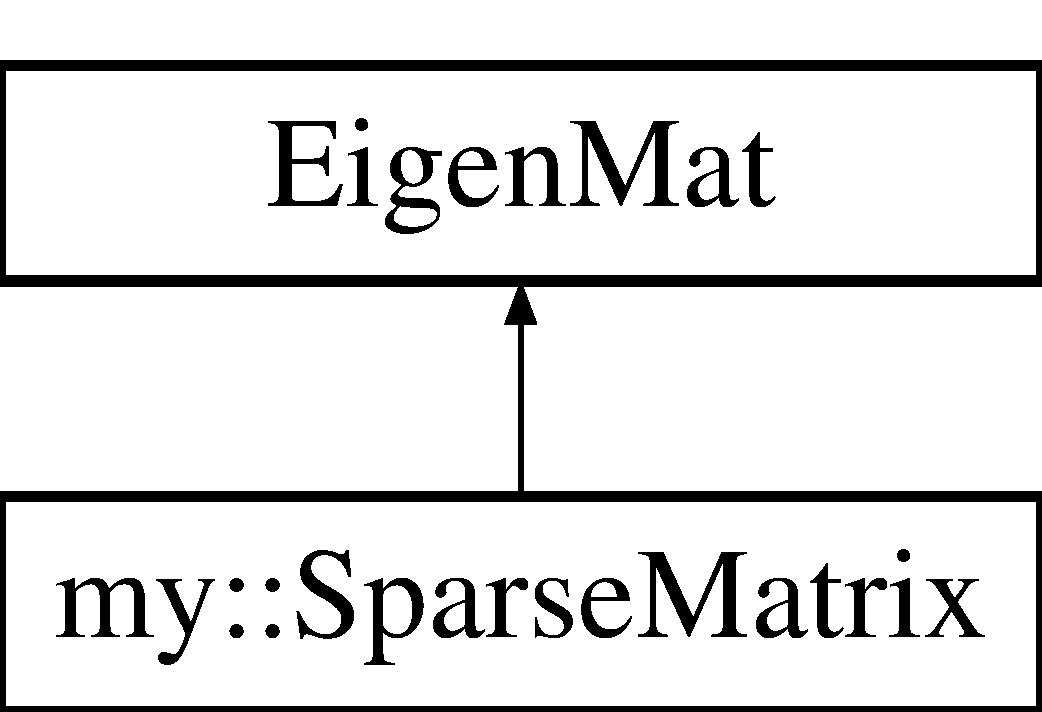
\includegraphics[height=2.000000cm]{classmy_1_1SparseMatrix}
\end{center}
\end{figure}
\subsection*{Public Member Functions}
\begin{DoxyCompactItemize}
\item 
\hyperlink{classmy_1_1SparseMatrix_a6d2ae114334791f63a3e44a96047285f}{Sparse\+Matrix} ()
\begin{DoxyCompactList}\small\item\em The Null constructor. \end{DoxyCompactList}\item 
\hyperlink{classmy_1_1SparseMatrix_a1de5bf243a6a7810cfc1a4395f304067}{Sparse\+Matrix} (const \hyperlink{namespacemy_a42365393c537edae1e89d20ff90d1923}{my\+::integer} \+\_\+ncol, const \hyperlink{namespacemy_a42365393c537edae1e89d20ff90d1923}{my\+::integer} \+\_\+nrow)
\begin{DoxyCompactList}\small\item\em The Default constructor. \end{DoxyCompactList}\item 
void \hyperlink{classmy_1_1SparseMatrix_a9055b71f0d6dbe001608977acf951c60}{Reserve} (const \hyperlink{namespacemy_a42365393c537edae1e89d20ff90d1923}{my\+::integer} \+\_\+size)
\begin{DoxyCompactList}\small\item\em Reserve an stimated ammount of memory for the sparse matrix. \end{DoxyCompactList}\item 
\hyperlink{namespacemy_a42365393c537edae1e89d20ff90d1923}{my\+::integer} \hyperlink{classmy_1_1SparseMatrix_a63704d3902b5640a64a7d25afcd28d85}{Num\+Raw\+Entries} () const 
\begin{DoxyCompactList}\small\item\em Returns the total number of raw entries in the matrix. \end{DoxyCompactList}\item 
void \hyperlink{classmy_1_1SparseMatrix_a99dd255132d7af8e313723f91f08cf80}{Add\+New\+Raw\+Entry} (const \hyperlink{namespacesparse_a841919761b2e35cc4d59f636ab10a07b}{sparse\+::\+Entry} \+\_\+triplet)
\begin{DoxyCompactList}\small\item\em Add a new Raw entry in the matrix. \end{DoxyCompactList}\item 
void \hyperlink{classmy_1_1SparseMatrix_a1f3d02071e55da946a9a26a65615aa8f}{Set\+From\+Raw\+Entries} ()
\begin{DoxyCompactList}\small\item\em Set the sparse matrix using the raw\+\_\+entries. \end{DoxyCompactList}\item 
\hyperlink{namespacesparse_a841919761b2e35cc4d59f636ab10a07b}{sparse\+::\+Entry} \hyperlink{classmy_1_1SparseMatrix_a0dbde5c277c46a89b62e48fb67d4db0a}{Raw\+Entry} (const \hyperlink{namespacemy_a42365393c537edae1e89d20ff90d1923}{my\+::integer} \+\_\+idx) const 
\item 
\hyperlink{namespacesparse_a841919761b2e35cc4d59f636ab10a07b}{sparse\+::\+Entry} \& \hyperlink{classmy_1_1SparseMatrix_adf8d262ff470f14d838eecad0665b6e9}{Raw\+Entry} (const \hyperlink{namespacemy_a42365393c537edae1e89d20ff90d1923}{my\+::integer} \+\_\+idx)
\item 
bool \hyperlink{classmy_1_1SparseMatrix_a441853d16d18e7f1e719c1d88258e637}{Is\+Set} () const 
\end{DoxyCompactItemize}
\subsection*{Private Attributes}
\begin{DoxyCompactItemize}
\item 
std\+::vector$<$ \hyperlink{namespacesparse_a841919761b2e35cc4d59f636ab10a07b}{sparse\+::\+Entry} $>$ \hyperlink{classmy_1_1SparseMatrix_a00427b5f489a6d2c5dd42e59439c2782}{mat\+Entry\+\_\+}
\item 
bool \hyperlink{classmy_1_1SparseMatrix_a19cd30efa5d59bf9cc1b6343e5acc392}{matrix\+\_\+is\+\_\+set\+\_\+}
\end{DoxyCompactItemize}


\subsection{Detailed Description}
The Sparse Matrix Class. Inheritated from \hyperlink{namespacesparse_af3fe1ceb08995f6d08e5f96fbbe021bf}{sparse\+::\+Eigen\+Mat}. 

\subsection{Constructor \& Destructor Documentation}
\hypertarget{classmy_1_1SparseMatrix_a6d2ae114334791f63a3e44a96047285f}{\index{my\+::\+Sparse\+Matrix@{my\+::\+Sparse\+Matrix}!Sparse\+Matrix@{Sparse\+Matrix}}
\index{Sparse\+Matrix@{Sparse\+Matrix}!my\+::\+Sparse\+Matrix@{my\+::\+Sparse\+Matrix}}
\subsubsection[{Sparse\+Matrix}]{\setlength{\rightskip}{0pt plus 5cm}my\+::\+Sparse\+Matrix\+::\+Sparse\+Matrix (
\begin{DoxyParamCaption}
{}
\end{DoxyParamCaption}
)\hspace{0.3cm}{\ttfamily [inline]}}}\label{classmy_1_1SparseMatrix_a6d2ae114334791f63a3e44a96047285f}


The Null constructor. 

\hypertarget{classmy_1_1SparseMatrix_a1de5bf243a6a7810cfc1a4395f304067}{\index{my\+::\+Sparse\+Matrix@{my\+::\+Sparse\+Matrix}!Sparse\+Matrix@{Sparse\+Matrix}}
\index{Sparse\+Matrix@{Sparse\+Matrix}!my\+::\+Sparse\+Matrix@{my\+::\+Sparse\+Matrix}}
\subsubsection[{Sparse\+Matrix}]{\setlength{\rightskip}{0pt plus 5cm}my\+::\+Sparse\+Matrix\+::\+Sparse\+Matrix (
\begin{DoxyParamCaption}
\item[{const {\bf my\+::integer}}]{\+\_\+ncol, }
\item[{const {\bf my\+::integer}}]{\+\_\+nrow}
\end{DoxyParamCaption}
)\hspace{0.3cm}{\ttfamily [inline]}}}\label{classmy_1_1SparseMatrix_a1de5bf243a6a7810cfc1a4395f304067}


The Default constructor. 



\subsection{Member Function Documentation}
\hypertarget{classmy_1_1SparseMatrix_a99dd255132d7af8e313723f91f08cf80}{\index{my\+::\+Sparse\+Matrix@{my\+::\+Sparse\+Matrix}!Add\+New\+Raw\+Entry@{Add\+New\+Raw\+Entry}}
\index{Add\+New\+Raw\+Entry@{Add\+New\+Raw\+Entry}!my\+::\+Sparse\+Matrix@{my\+::\+Sparse\+Matrix}}
\subsubsection[{Add\+New\+Raw\+Entry}]{\setlength{\rightskip}{0pt plus 5cm}void my\+::\+Sparse\+Matrix\+::\+Add\+New\+Raw\+Entry (
\begin{DoxyParamCaption}
\item[{const {\bf sparse\+::\+Entry}}]{\+\_\+triplet}
\end{DoxyParamCaption}
)\hspace{0.3cm}{\ttfamily [inline]}}}\label{classmy_1_1SparseMatrix_a99dd255132d7af8e313723f91f08cf80}


Add a new Raw entry in the matrix. 

This method will append a new entry to the entry list, not making any check on the previous entries \hypertarget{classmy_1_1SparseMatrix_a441853d16d18e7f1e719c1d88258e637}{\index{my\+::\+Sparse\+Matrix@{my\+::\+Sparse\+Matrix}!Is\+Set@{Is\+Set}}
\index{Is\+Set@{Is\+Set}!my\+::\+Sparse\+Matrix@{my\+::\+Sparse\+Matrix}}
\subsubsection[{Is\+Set}]{\setlength{\rightskip}{0pt plus 5cm}bool my\+::\+Sparse\+Matrix\+::\+Is\+Set (
\begin{DoxyParamCaption}
{}
\end{DoxyParamCaption}
) const\hspace{0.3cm}{\ttfamily [inline]}}}\label{classmy_1_1SparseMatrix_a441853d16d18e7f1e719c1d88258e637}
\hypertarget{classmy_1_1SparseMatrix_a63704d3902b5640a64a7d25afcd28d85}{\index{my\+::\+Sparse\+Matrix@{my\+::\+Sparse\+Matrix}!Num\+Raw\+Entries@{Num\+Raw\+Entries}}
\index{Num\+Raw\+Entries@{Num\+Raw\+Entries}!my\+::\+Sparse\+Matrix@{my\+::\+Sparse\+Matrix}}
\subsubsection[{Num\+Raw\+Entries}]{\setlength{\rightskip}{0pt plus 5cm}{\bf my\+::integer} my\+::\+Sparse\+Matrix\+::\+Num\+Raw\+Entries (
\begin{DoxyParamCaption}
{}
\end{DoxyParamCaption}
) const\hspace{0.3cm}{\ttfamily [inline]}}}\label{classmy_1_1SparseMatrix_a63704d3902b5640a64a7d25afcd28d85}


Returns the total number of raw entries in the matrix. 

Returns the total number of raw entries in the matrix. This method will count repeated and non-\/zero entries \hypertarget{classmy_1_1SparseMatrix_a0dbde5c277c46a89b62e48fb67d4db0a}{\index{my\+::\+Sparse\+Matrix@{my\+::\+Sparse\+Matrix}!Raw\+Entry@{Raw\+Entry}}
\index{Raw\+Entry@{Raw\+Entry}!my\+::\+Sparse\+Matrix@{my\+::\+Sparse\+Matrix}}
\subsubsection[{Raw\+Entry}]{\setlength{\rightskip}{0pt plus 5cm}{\bf sparse\+::\+Entry} my\+::\+Sparse\+Matrix\+::\+Raw\+Entry (
\begin{DoxyParamCaption}
\item[{const {\bf my\+::integer}}]{\+\_\+idx}
\end{DoxyParamCaption}
) const\hspace{0.3cm}{\ttfamily [inline]}}}\label{classmy_1_1SparseMatrix_a0dbde5c277c46a89b62e48fb67d4db0a}
\hypertarget{classmy_1_1SparseMatrix_adf8d262ff470f14d838eecad0665b6e9}{\index{my\+::\+Sparse\+Matrix@{my\+::\+Sparse\+Matrix}!Raw\+Entry@{Raw\+Entry}}
\index{Raw\+Entry@{Raw\+Entry}!my\+::\+Sparse\+Matrix@{my\+::\+Sparse\+Matrix}}
\subsubsection[{Raw\+Entry}]{\setlength{\rightskip}{0pt plus 5cm}{\bf sparse\+::\+Entry}\& my\+::\+Sparse\+Matrix\+::\+Raw\+Entry (
\begin{DoxyParamCaption}
\item[{const {\bf my\+::integer}}]{\+\_\+idx}
\end{DoxyParamCaption}
)\hspace{0.3cm}{\ttfamily [inline]}}}\label{classmy_1_1SparseMatrix_adf8d262ff470f14d838eecad0665b6e9}
\hypertarget{classmy_1_1SparseMatrix_a9055b71f0d6dbe001608977acf951c60}{\index{my\+::\+Sparse\+Matrix@{my\+::\+Sparse\+Matrix}!Reserve@{Reserve}}
\index{Reserve@{Reserve}!my\+::\+Sparse\+Matrix@{my\+::\+Sparse\+Matrix}}
\subsubsection[{Reserve}]{\setlength{\rightskip}{0pt plus 5cm}void my\+::\+Sparse\+Matrix\+::\+Reserve (
\begin{DoxyParamCaption}
\item[{const {\bf my\+::integer}}]{\+\_\+size}
\end{DoxyParamCaption}
)\hspace{0.3cm}{\ttfamily [inline]}}}\label{classmy_1_1SparseMatrix_a9055b71f0d6dbe001608977acf951c60}


Reserve an stimated ammount of memory for the sparse matrix. 

\hypertarget{classmy_1_1SparseMatrix_a1f3d02071e55da946a9a26a65615aa8f}{\index{my\+::\+Sparse\+Matrix@{my\+::\+Sparse\+Matrix}!Set\+From\+Raw\+Entries@{Set\+From\+Raw\+Entries}}
\index{Set\+From\+Raw\+Entries@{Set\+From\+Raw\+Entries}!my\+::\+Sparse\+Matrix@{my\+::\+Sparse\+Matrix}}
\subsubsection[{Set\+From\+Raw\+Entries}]{\setlength{\rightskip}{0pt plus 5cm}void my\+::\+Sparse\+Matrix\+::\+Set\+From\+Raw\+Entries (
\begin{DoxyParamCaption}
{}
\end{DoxyParamCaption}
)\hspace{0.3cm}{\ttfamily [inline]}}}\label{classmy_1_1SparseMatrix_a1f3d02071e55da946a9a26a65615aa8f}


Set the sparse matrix using the raw\+\_\+entries. 

The list of entries after this operation is destroyed 

\subsection{Member Data Documentation}
\hypertarget{classmy_1_1SparseMatrix_a00427b5f489a6d2c5dd42e59439c2782}{\index{my\+::\+Sparse\+Matrix@{my\+::\+Sparse\+Matrix}!mat\+Entry\+\_\+@{mat\+Entry\+\_\+}}
\index{mat\+Entry\+\_\+@{mat\+Entry\+\_\+}!my\+::\+Sparse\+Matrix@{my\+::\+Sparse\+Matrix}}
\subsubsection[{mat\+Entry\+\_\+}]{\setlength{\rightskip}{0pt plus 5cm}std\+::vector$<${\bf sparse\+::\+Entry}$>$ my\+::\+Sparse\+Matrix\+::mat\+Entry\+\_\+\hspace{0.3cm}{\ttfamily [private]}}}\label{classmy_1_1SparseMatrix_a00427b5f489a6d2c5dd42e59439c2782}
\hypertarget{classmy_1_1SparseMatrix_a19cd30efa5d59bf9cc1b6343e5acc392}{\index{my\+::\+Sparse\+Matrix@{my\+::\+Sparse\+Matrix}!matrix\+\_\+is\+\_\+set\+\_\+@{matrix\+\_\+is\+\_\+set\+\_\+}}
\index{matrix\+\_\+is\+\_\+set\+\_\+@{matrix\+\_\+is\+\_\+set\+\_\+}!my\+::\+Sparse\+Matrix@{my\+::\+Sparse\+Matrix}}
\subsubsection[{matrix\+\_\+is\+\_\+set\+\_\+}]{\setlength{\rightskip}{0pt plus 5cm}bool my\+::\+Sparse\+Matrix\+::matrix\+\_\+is\+\_\+set\+\_\+\hspace{0.3cm}{\ttfamily [private]}}}\label{classmy_1_1SparseMatrix_a19cd30efa5d59bf9cc1b6343e5acc392}


The documentation for this class was generated from the following file\+:\begin{DoxyCompactItemize}
\item 
/home/jgarcia/\+Dropbox/git-\/save/\+T\+B-\/\+Quantum\+Transp/include/\hyperlink{sparse__matrix_8hpp}{sparse\+\_\+matrix.\+hpp}\end{DoxyCompactItemize}

\chapter{File Documentation}
\hypertarget{homepage_8dox}{\section{homepage.\+dox File Reference}
\label{homepage_8dox}\index{homepage.\+dox@{homepage.\+dox}}
}

\hypertarget{fourier__transform_8cpp}{\section{/home/jgarcia/\+Dropbox/git-\/save/\+T\+B-\/\+Quantum\+Transp/fourier/fourier\+\_\+transform.cpp File Reference}
\label{fourier__transform_8cpp}\index{/home/jgarcia/\+Dropbox/git-\/save/\+T\+B-\/\+Quantum\+Transp/fourier/fourier\+\_\+transform.\+cpp@{/home/jgarcia/\+Dropbox/git-\/save/\+T\+B-\/\+Quantum\+Transp/fourier/fourier\+\_\+transform.\+cpp}}
}
{\ttfamily \#include \char`\"{}fourier\+\_\+transform.\+hpp\char`\"{}}\\*

\hypertarget{fourier__transform_8hpp}{\section{/home/jgarcia/\+Dropbox/git-\/save/\+T\+B-\/\+Quantum\+Transp/fourier/fourier\+\_\+transform.hpp File Reference}
\label{fourier__transform_8hpp}\index{/home/jgarcia/\+Dropbox/git-\/save/\+T\+B-\/\+Quantum\+Transp/fourier/fourier\+\_\+transform.\+hpp@{/home/jgarcia/\+Dropbox/git-\/save/\+T\+B-\/\+Quantum\+Transp/fourier/fourier\+\_\+transform.\+hpp}}
}
{\ttfamily \#include $<$vector$>$}\\*
{\ttfamily \#include $<$iostream$>$}\\*
{\ttfamily \#include $<$cstdio$>$}\\*
{\ttfamily \#include $<$cstdlib$>$}\\*
{\ttfamily \#include \char`\"{}types\+\_\+definitions.\+hpp\char`\"{}}\\*
{\ttfamily \#include \char`\"{}mkl\+\_\+types.\+h\char`\"{}}\\*
{\ttfamily \#include \char`\"{}mkl.\+h\char`\"{}}\\*
{\ttfamily \#include \char`\"{}mkl\+\_\+service.\+h\char`\"{}}\\*
{\ttfamily \#include \char`\"{}mkl\+\_\+dfti.\+h\char`\"{}}\\*
\subsection*{Namespaces}
\begin{DoxyCompactItemize}
\item 
 \hyperlink{namespacemkl}{mkl}
\end{DoxyCompactItemize}
\subsection*{Macros}
\begin{DoxyCompactItemize}
\item 
\#define \hyperlink{fourier__transform_8hpp_a1fa119034fee07a6d5449926cbb7915a}{M\+K\+L\+\_\+\+Complex16}~std\+::complex$<$double$>$
\item 
\#define \hyperlink{fourier__transform_8hpp_a0b45f62ef34311fdb79b8de82d75c0d3}{M\+K\+L\+\_\+\+Complex8}~std\+::complex$<$float$>$
\end{DoxyCompactItemize}
\subsection*{Functions}
\begin{DoxyCompactItemize}
\item 
void \hyperlink{namespacemkl_a122f328e6079ba392e8a44c1de72ca7f}{mkl\+::direct\+\_\+\+F\+F\+T} (D\+F\+T\+I\+\_\+\+D\+E\+S\+C\+R\+I\+P\+T\+O\+R\+\_\+\+H\+A\+N\+D\+L\+E \&dft\+\_\+handle, const \hyperlink{namespacemy_a42365393c537edae1e89d20ff90d1923}{my\+::integer} \+\_\+dim0, const \hyperlink{namespacemy_a42365393c537edae1e89d20ff90d1923}{my\+::integer} \+\_\+dim1, const \hyperlink{namespacemy_a42365393c537edae1e89d20ff90d1923}{my\+::integer} \+\_\+dim2, std\+::complex$<$ float $>$ $\ast$\+\_\+\+A)
\item 
void \hyperlink{namespacemkl_ad2c0764c53d2daac345314013c579080}{mkl\+::inverse\+\_\+\+F\+F\+T} (D\+F\+T\+I\+\_\+\+D\+E\+S\+C\+R\+I\+P\+T\+O\+R\+\_\+\+H\+A\+N\+D\+L\+E \&dft\+\_\+handle, const \hyperlink{namespacemy_a42365393c537edae1e89d20ff90d1923}{my\+::integer} \+\_\+dim0, const \hyperlink{namespacemy_a42365393c537edae1e89d20ff90d1923}{my\+::integer} \+\_\+dim1, const \hyperlink{namespacemy_a42365393c537edae1e89d20ff90d1923}{my\+::integer} \+\_\+dim2, std\+::complex$<$ float $>$ $\ast$\+\_\+\+A)
\end{DoxyCompactItemize}


\subsection{Macro Definition Documentation}
\hypertarget{fourier__transform_8hpp_a1fa119034fee07a6d5449926cbb7915a}{\index{fourier\+\_\+transform.\+hpp@{fourier\+\_\+transform.\+hpp}!M\+K\+L\+\_\+\+Complex16@{M\+K\+L\+\_\+\+Complex16}}
\index{M\+K\+L\+\_\+\+Complex16@{M\+K\+L\+\_\+\+Complex16}!fourier\+\_\+transform.\+hpp@{fourier\+\_\+transform.\+hpp}}
\subsubsection[{M\+K\+L\+\_\+\+Complex16}]{\setlength{\rightskip}{0pt plus 5cm}\#define M\+K\+L\+\_\+\+Complex16~std\+::complex$<$double$>$}}\label{fourier__transform_8hpp_a1fa119034fee07a6d5449926cbb7915a}
\hypertarget{fourier__transform_8hpp_a0b45f62ef34311fdb79b8de82d75c0d3}{\index{fourier\+\_\+transform.\+hpp@{fourier\+\_\+transform.\+hpp}!M\+K\+L\+\_\+\+Complex8@{M\+K\+L\+\_\+\+Complex8}}
\index{M\+K\+L\+\_\+\+Complex8@{M\+K\+L\+\_\+\+Complex8}!fourier\+\_\+transform.\+hpp@{fourier\+\_\+transform.\+hpp}}
\subsubsection[{M\+K\+L\+\_\+\+Complex8}]{\setlength{\rightskip}{0pt plus 5cm}\#define M\+K\+L\+\_\+\+Complex8~std\+::complex$<$float$>$}}\label{fourier__transform_8hpp_a0b45f62ef34311fdb79b8de82d75c0d3}

\hypertarget{custom__random_8hpp}{\section{/home/jgarcia/\+Dropbox/git-\/save/\+T\+B-\/\+Quantum\+Transp/include/custom\+\_\+random.hpp File Reference}
\label{custom__random_8hpp}\index{/home/jgarcia/\+Dropbox/git-\/save/\+T\+B-\/\+Quantum\+Transp/include/custom\+\_\+random.\+hpp@{/home/jgarcia/\+Dropbox/git-\/save/\+T\+B-\/\+Quantum\+Transp/include/custom\+\_\+random.\+hpp}}
}
{\ttfamily \#include $<$boost/random/mersenne\+\_\+twister.\+hpp$>$}\\*
{\ttfamily \#include $<$boost/random/uniform\+\_\+real\+\_\+distribution.\+hpp$>$}\\*
\subsection*{Namespaces}
\begin{DoxyCompactItemize}
\item 
 \hyperlink{namespacecustom__random}{custom\+\_\+random}
\end{DoxyCompactItemize}
\subsection*{Typedefs}
\begin{DoxyCompactItemize}
\item 
typedef \\*
boost\+::random\+::uniform\+\_\+real\+\_\+distribution\\*
$<$ \hyperlink{namespacemy_ad61baeaeda728a4c48dd64f93e44a46c}{my\+::real} $>$ \hyperlink{namespacecustom__random_aabaaf85a6342ff33004ff1ba5eaf9014}{custom\+\_\+random\+::uniform\+\_\+real\+\_\+dist}
\item 
typedef boost\+::random\+::mt19937 \hyperlink{namespacecustom__random_a46f0cd4be260de20f93531f3f9c1a2f6}{custom\+\_\+random\+::generator}
\end{DoxyCompactItemize}

\hypertarget{efficient__mod_8hpp}{\section{/home/jgarcia/\+Dropbox/git-\/save/\+T\+B-\/\+Quantum\+Transp/include/efficient\+\_\+mod.hpp File Reference}
\label{efficient__mod_8hpp}\index{/home/jgarcia/\+Dropbox/git-\/save/\+T\+B-\/\+Quantum\+Transp/include/efficient\+\_\+mod.\+hpp@{/home/jgarcia/\+Dropbox/git-\/save/\+T\+B-\/\+Quantum\+Transp/include/efficient\+\_\+mod.\+hpp}}
}
{\ttfamily \#include \char`\"{}types\+\_\+definitions.\+hpp\char`\"{}}\\*
\subsection*{Functions}
\begin{DoxyCompactItemize}
\item 
\hyperlink{namespacemy_a42365393c537edae1e89d20ff90d1923}{my\+::integer} \hyperlink{efficient__mod_8hpp_a8fcfdf46a525bf8ba9039f25ac55f1d0}{Eff\+Mod} (\hyperlink{namespacemy_a42365393c537edae1e89d20ff90d1923}{my\+::integer} i, \hyperlink{namespacemy_a42365393c537edae1e89d20ff90d1923}{my\+::integer} size)
\end{DoxyCompactItemize}


\subsection{Function Documentation}
\hypertarget{efficient__mod_8hpp_a8fcfdf46a525bf8ba9039f25ac55f1d0}{\index{efficient\+\_\+mod.\+hpp@{efficient\+\_\+mod.\+hpp}!Eff\+Mod@{Eff\+Mod}}
\index{Eff\+Mod@{Eff\+Mod}!efficient\+\_\+mod.\+hpp@{efficient\+\_\+mod.\+hpp}}
\subsubsection[{Eff\+Mod}]{\setlength{\rightskip}{0pt plus 5cm}{\bf my\+::integer} Eff\+Mod (
\begin{DoxyParamCaption}
\item[{{\bf my\+::integer}}]{i, }
\item[{{\bf my\+::integer}}]{size}
\end{DoxyParamCaption}
)\hspace{0.3cm}{\ttfamily [inline]}}}\label{efficient__mod_8hpp_a8fcfdf46a525bf8ba9039f25ac55f1d0}

\hypertarget{lattice__geometry_8h}{\section{/home/jgarcia/\+Dropbox/git-\/save/\+T\+B-\/\+Quantum\+Transp/include/lattice\+\_\+geometry.h File Reference}
\label{lattice__geometry_8h}\index{/home/jgarcia/\+Dropbox/git-\/save/\+T\+B-\/\+Quantum\+Transp/include/lattice\+\_\+geometry.\+h@{/home/jgarcia/\+Dropbox/git-\/save/\+T\+B-\/\+Quantum\+Transp/include/lattice\+\_\+geometry.\+h}}
}
{\ttfamily \#include \char`\"{}types\+\_\+definitions.\+hpp\char`\"{}}\\*

\hypertarget{mpi__util_8hpp}{\section{/home/jgarcia/\+Dropbox/git-\/save/\+T\+B-\/\+Quantum\+Transp/include/mpi\+\_\+util.hpp File Reference}
\label{mpi__util_8hpp}\index{/home/jgarcia/\+Dropbox/git-\/save/\+T\+B-\/\+Quantum\+Transp/include/mpi\+\_\+util.\+hpp@{/home/jgarcia/\+Dropbox/git-\/save/\+T\+B-\/\+Quantum\+Transp/include/mpi\+\_\+util.\+hpp}}
}
{\ttfamily \#include \char`\"{}mpi.\+h\char`\"{}}\\*
{\ttfamily \#include $<$cmath$>$}\\*
{\ttfamily \#include $<$iostream$>$}\\*
{\ttfamily \#include $<$string$>$}\\*
\subsection*{Classes}
\begin{DoxyCompactItemize}
\item 
class \hyperlink{classNumCal_1_1cout__class}{Num\+Cal\+::cout\+\_\+class}
\item 
class \hyperlink{classNumCal_1_1cerr__class}{Num\+Cal\+::cerr\+\_\+class}
\end{DoxyCompactItemize}
\subsection*{Namespaces}
\begin{DoxyCompactItemize}
\item 
 \hyperlink{namespaceNumCal}{Num\+Cal}
\end{DoxyCompactItemize}
\subsection*{Macros}
\begin{DoxyCompactItemize}
\item 
\#define \hyperlink{mpi__util_8hpp_a780f39e5ce1ec856f71c8329db6f7ce9}{N\+U\+M\+C\+A\+L\+\_\+\+M\+P\+I\+\_\+\+I\+N\+I\+T}()~M\+P\+I\+::\+Init ()
\item 
\#define \hyperlink{mpi__util_8hpp_a6bbbec00d5cf914bf3b8eb6b7359ce8f}{N\+U\+M\+C\+A\+L\+\_\+\+M\+P\+I\+\_\+\+F\+I\+N\+A\+L\+I\+Z\+E}()~M\+P\+I\+::\+Finalize ( )
\item 
\#define \hyperlink{mpi__util_8hpp_ac1b3e3d6892a03ab0b30207236b16c6f}{N\+U\+M\+C\+A\+L\+\_\+\+M\+P\+I\+\_\+\+G\+E\+T\+R\+A\+N\+K}()~M\+P\+I\+::\+C\+O\+M\+M\+\_\+\+W\+O\+R\+L\+D.\+Get\+\_\+rank ( )
\item 
\#define \hyperlink{mpi__util_8hpp_a7010754118e576a06b9f9ebc8c8667ab}{N\+U\+M\+C\+A\+L\+\_\+\+M\+P\+I\+\_\+\+G\+E\+T\+P\+R\+O\+C}()~M\+P\+I\+::\+C\+O\+M\+M\+\_\+\+W\+O\+R\+L\+D.\+Get\+\_\+size ( )
\end{DoxyCompactItemize}


\subsection{Macro Definition Documentation}
\hypertarget{mpi__util_8hpp_a6bbbec00d5cf914bf3b8eb6b7359ce8f}{\index{mpi\+\_\+util.\+hpp@{mpi\+\_\+util.\+hpp}!N\+U\+M\+C\+A\+L\+\_\+\+M\+P\+I\+\_\+\+F\+I\+N\+A\+L\+I\+Z\+E@{N\+U\+M\+C\+A\+L\+\_\+\+M\+P\+I\+\_\+\+F\+I\+N\+A\+L\+I\+Z\+E}}
\index{N\+U\+M\+C\+A\+L\+\_\+\+M\+P\+I\+\_\+\+F\+I\+N\+A\+L\+I\+Z\+E@{N\+U\+M\+C\+A\+L\+\_\+\+M\+P\+I\+\_\+\+F\+I\+N\+A\+L\+I\+Z\+E}!mpi\+\_\+util.\+hpp@{mpi\+\_\+util.\+hpp}}
\subsubsection[{N\+U\+M\+C\+A\+L\+\_\+\+M\+P\+I\+\_\+\+F\+I\+N\+A\+L\+I\+Z\+E}]{\setlength{\rightskip}{0pt plus 5cm}\#define N\+U\+M\+C\+A\+L\+\_\+\+M\+P\+I\+\_\+\+F\+I\+N\+A\+L\+I\+Z\+E(
\begin{DoxyParamCaption}
{}
\end{DoxyParamCaption}
)~M\+P\+I\+::\+Finalize ( )}}\label{mpi__util_8hpp_a6bbbec00d5cf914bf3b8eb6b7359ce8f}
\hypertarget{mpi__util_8hpp_a7010754118e576a06b9f9ebc8c8667ab}{\index{mpi\+\_\+util.\+hpp@{mpi\+\_\+util.\+hpp}!N\+U\+M\+C\+A\+L\+\_\+\+M\+P\+I\+\_\+\+G\+E\+T\+P\+R\+O\+C@{N\+U\+M\+C\+A\+L\+\_\+\+M\+P\+I\+\_\+\+G\+E\+T\+P\+R\+O\+C}}
\index{N\+U\+M\+C\+A\+L\+\_\+\+M\+P\+I\+\_\+\+G\+E\+T\+P\+R\+O\+C@{N\+U\+M\+C\+A\+L\+\_\+\+M\+P\+I\+\_\+\+G\+E\+T\+P\+R\+O\+C}!mpi\+\_\+util.\+hpp@{mpi\+\_\+util.\+hpp}}
\subsubsection[{N\+U\+M\+C\+A\+L\+\_\+\+M\+P\+I\+\_\+\+G\+E\+T\+P\+R\+O\+C}]{\setlength{\rightskip}{0pt plus 5cm}\#define N\+U\+M\+C\+A\+L\+\_\+\+M\+P\+I\+\_\+\+G\+E\+T\+P\+R\+O\+C(
\begin{DoxyParamCaption}
{}
\end{DoxyParamCaption}
)~M\+P\+I\+::\+C\+O\+M\+M\+\_\+\+W\+O\+R\+L\+D.\+Get\+\_\+size ( )}}\label{mpi__util_8hpp_a7010754118e576a06b9f9ebc8c8667ab}
\hypertarget{mpi__util_8hpp_ac1b3e3d6892a03ab0b30207236b16c6f}{\index{mpi\+\_\+util.\+hpp@{mpi\+\_\+util.\+hpp}!N\+U\+M\+C\+A\+L\+\_\+\+M\+P\+I\+\_\+\+G\+E\+T\+R\+A\+N\+K@{N\+U\+M\+C\+A\+L\+\_\+\+M\+P\+I\+\_\+\+G\+E\+T\+R\+A\+N\+K}}
\index{N\+U\+M\+C\+A\+L\+\_\+\+M\+P\+I\+\_\+\+G\+E\+T\+R\+A\+N\+K@{N\+U\+M\+C\+A\+L\+\_\+\+M\+P\+I\+\_\+\+G\+E\+T\+R\+A\+N\+K}!mpi\+\_\+util.\+hpp@{mpi\+\_\+util.\+hpp}}
\subsubsection[{N\+U\+M\+C\+A\+L\+\_\+\+M\+P\+I\+\_\+\+G\+E\+T\+R\+A\+N\+K}]{\setlength{\rightskip}{0pt plus 5cm}\#define N\+U\+M\+C\+A\+L\+\_\+\+M\+P\+I\+\_\+\+G\+E\+T\+R\+A\+N\+K(
\begin{DoxyParamCaption}
{}
\end{DoxyParamCaption}
)~M\+P\+I\+::\+C\+O\+M\+M\+\_\+\+W\+O\+R\+L\+D.\+Get\+\_\+rank ( )}}\label{mpi__util_8hpp_ac1b3e3d6892a03ab0b30207236b16c6f}
\hypertarget{mpi__util_8hpp_a780f39e5ce1ec856f71c8329db6f7ce9}{\index{mpi\+\_\+util.\+hpp@{mpi\+\_\+util.\+hpp}!N\+U\+M\+C\+A\+L\+\_\+\+M\+P\+I\+\_\+\+I\+N\+I\+T@{N\+U\+M\+C\+A\+L\+\_\+\+M\+P\+I\+\_\+\+I\+N\+I\+T}}
\index{N\+U\+M\+C\+A\+L\+\_\+\+M\+P\+I\+\_\+\+I\+N\+I\+T@{N\+U\+M\+C\+A\+L\+\_\+\+M\+P\+I\+\_\+\+I\+N\+I\+T}!mpi\+\_\+util.\+hpp@{mpi\+\_\+util.\+hpp}}
\subsubsection[{N\+U\+M\+C\+A\+L\+\_\+\+M\+P\+I\+\_\+\+I\+N\+I\+T}]{\setlength{\rightskip}{0pt plus 5cm}\#define N\+U\+M\+C\+A\+L\+\_\+\+M\+P\+I\+\_\+\+I\+N\+I\+T(
\begin{DoxyParamCaption}
{}
\end{DoxyParamCaption}
)~M\+P\+I\+::\+Init ()}}\label{mpi__util_8hpp_a780f39e5ce1ec856f71c8329db6f7ce9}

\hypertarget{sparse__matrix_8hpp}{\section{/home/jgarcia/\+Dropbox/git-\/save/\+T\+B-\/\+Quantum\+Transp/include/sparse\+\_\+matrix.hpp File Reference}
\label{sparse__matrix_8hpp}\index{/home/jgarcia/\+Dropbox/git-\/save/\+T\+B-\/\+Quantum\+Transp/include/sparse\+\_\+matrix.\+hpp@{/home/jgarcia/\+Dropbox/git-\/save/\+T\+B-\/\+Quantum\+Transp/include/sparse\+\_\+matrix.\+hpp}}
}
{\ttfamily \#include $<$vector$>$}\\*
{\ttfamily \#include \char`\"{}Eigen/\+Sparse\char`\"{}}\\*
{\ttfamily \#include \char`\"{}types\+\_\+definitions.\+hpp\char`\"{}}\\*
\subsection*{Classes}
\begin{DoxyCompactItemize}
\item 
class \hyperlink{classmy_1_1SparseMatrix}{my\+::\+Sparse\+Matrix}
\begin{DoxyCompactList}\small\item\em The Sparse Matrix Class. Inheritated from \hyperlink{namespacesparse_af3fe1ceb08995f6d08e5f96fbbe021bf}{sparse\+::\+Eigen\+Mat}. \end{DoxyCompactList}\end{DoxyCompactItemize}
\subsection*{Namespaces}
\begin{DoxyCompactItemize}
\item 
 \hyperlink{namespacesparse}{sparse}
\begin{DoxyCompactList}\small\item\em Defines the std\+::vector class. \end{DoxyCompactList}\item 
 \hyperlink{namespacemy}{my}
\begin{DoxyCompactList}\small\item\em Namespace for the classes created for this project. \end{DoxyCompactList}\end{DoxyCompactItemize}
\subsection*{Typedefs}
\begin{DoxyCompactItemize}
\item 
typedef Eigen\+::\+Sparse\+Matrix\\*
$<$ \hyperlink{namespacemy_a12d9dde7e2fb58fbd11051705c382a86}{my\+::scalar}, Eigen\+::\+Row\+Major, \\*
\hyperlink{namespacemy_a42365393c537edae1e89d20ff90d1923}{my\+::integer} $>$ \hyperlink{namespacesparse_af3fe1ceb08995f6d08e5f96fbbe021bf}{sparse\+::\+Eigen\+Mat}
\item 
typedef Eigen\+::\+Triplet\\*
$<$ \hyperlink{namespacemy_a12d9dde7e2fb58fbd11051705c382a86}{my\+::scalar} $>$ \hyperlink{namespacesparse_a841919761b2e35cc4d59f636ab10a07b}{sparse\+::\+Entry}
\end{DoxyCompactItemize}

\hypertarget{string__utilities_8hpp}{\section{/home/jgarcia/\+Dropbox/git-\/save/\+T\+B-\/\+Quantum\+Transp/include/string\+\_\+utilities.hpp File Reference}
\label{string__utilities_8hpp}\index{/home/jgarcia/\+Dropbox/git-\/save/\+T\+B-\/\+Quantum\+Transp/include/string\+\_\+utilities.\+hpp@{/home/jgarcia/\+Dropbox/git-\/save/\+T\+B-\/\+Quantum\+Transp/include/string\+\_\+utilities.\+hpp}}
}
{\ttfamily \#include $<$string$>$}\\*
{\ttfamily \#include $<$cstring$>$}\\*
\subsection*{Namespaces}
\begin{DoxyCompactItemize}
\item 
 \hyperlink{namespaceNumCal}{Num\+Cal}
\item 
 \hyperlink{namespaceNumCal_1_1stringUtil}{Num\+Cal\+::string\+Util}
\end{DoxyCompactItemize}
\subsection*{Functions}
\begin{DoxyCompactItemize}
\item 
bool \hyperlink{namespaceNumCal_1_1stringUtil_aa0efe6ff36e75d81d5747ca4af3457ba}{Num\+Cal\+::string\+Util\+::\+Is\+Integer} (const std\+::string \&s)
\item 
bool \hyperlink{namespaceNumCal_1_1stringUtil_a8d5b407d709aa07480da49d070e84b00}{Num\+Cal\+::string\+Util\+::\+Is\+Number} (const std\+::string \&s)
\end{DoxyCompactItemize}

\hypertarget{timing_8hpp}{\section{/home/jgarcia/\+Dropbox/git-\/save/\+T\+B-\/\+Quantum\+Transp/include/timing.hpp File Reference}
\label{timing_8hpp}\index{/home/jgarcia/\+Dropbox/git-\/save/\+T\+B-\/\+Quantum\+Transp/include/timing.\+hpp@{/home/jgarcia/\+Dropbox/git-\/save/\+T\+B-\/\+Quantum\+Transp/include/timing.\+hpp}}
}
{\ttfamily \#include $<$ctime$>$}\\*
{\ttfamily \#include $<$cstdio$>$}\\*

\hypertarget{types__definitions_8hpp}{\section{/home/jgarcia/\+Dropbox/git-\/save/\+T\+B-\/\+Quantum\+Transp/include/types\+\_\+definitions.hpp File Reference}
\label{types__definitions_8hpp}\index{/home/jgarcia/\+Dropbox/git-\/save/\+T\+B-\/\+Quantum\+Transp/include/types\+\_\+definitions.\+hpp@{/home/jgarcia/\+Dropbox/git-\/save/\+T\+B-\/\+Quantum\+Transp/include/types\+\_\+definitions.\+hpp}}
}
{\ttfamily \#include \char`\"{}Eigen/\+Sparse\char`\"{}}\\*
{\ttfamily \#include $<$complex$>$}\\*
{\ttfamily \#include $<$vector$>$}\\*
\subsection*{Namespaces}
\begin{DoxyCompactItemize}
\item 
 \hyperlink{namespacemy}{my}
\begin{DoxyCompactList}\small\item\em Namespace for the classes created for this project. \end{DoxyCompactList}\item 
 \hyperlink{namespaceNumCal}{Num\+Cal}
\end{DoxyCompactItemize}
\subsection*{Typedefs}
\begin{DoxyCompactItemize}
\item 
typedef float \hyperlink{types__definitions_8hpp_afcf02aefd75cea1c0178a18bbfcb3d1a}{external\+\_\+real}
\item 
typedef std\+::complex\\*
$<$ \hyperlink{types__definitions_8hpp_afcf02aefd75cea1c0178a18bbfcb3d1a}{external\+\_\+real} $>$ \hyperlink{types__definitions_8hpp_a4c933564179b32b78cb338ca417616a8}{external\+\_\+complex}
\item 
typedef std\+::complex\\*
$<$ \hyperlink{types__definitions_8hpp_afcf02aefd75cea1c0178a18bbfcb3d1a}{external\+\_\+real} $>$ \hyperlink{types__definitions_8hpp_af5c52aebac57703de05e631d36a8ef2e}{external\+\_\+scalar}
\item 
typedef std\+::vector\\*
$<$ \hyperlink{types__definitions_8hpp_af5c52aebac57703de05e631d36a8ef2e}{external\+\_\+scalar} $>$ \hyperlink{types__definitions_8hpp_aea218327e998c8c8c583f91564afd1b4}{external\+\_\+vector}
\item 
typedef std\+::vector\\*
$<$ \hyperlink{types__definitions_8hpp_af5c52aebac57703de05e631d36a8ef2e}{external\+\_\+scalar} $>$ \hyperlink{types__definitions_8hpp_ac4a55bdf0574672fe1bf23fe295feaf4}{external\+\_\+dvector}
\item 
typedef \hyperlink{types__definitions_8hpp_afcf02aefd75cea1c0178a18bbfcb3d1a}{external\+\_\+real} \hyperlink{namespacemy_ad61baeaeda728a4c48dd64f93e44a46c}{my\+::real}
\item 
typedef unsigned long \hyperlink{namespacemy_ac9e2c9fc46dc44ed285976e482ee6ef4}{my\+::size\+\_\+t}
\item 
typedef int \hyperlink{namespacemy_a42365393c537edae1e89d20ff90d1923}{my\+::integer}
\item 
typedef \hyperlink{types__definitions_8hpp_a4c933564179b32b78cb338ca417616a8}{external\+\_\+complex} \hyperlink{namespacemy_a1ed6ea9ef51c0aa31f8b671fb04d758f}{my\+::complex}
\item 
typedef \hyperlink{types__definitions_8hpp_af5c52aebac57703de05e631d36a8ef2e}{external\+\_\+scalar} \hyperlink{namespacemy_a12d9dde7e2fb58fbd11051705c382a86}{my\+::scalar}
\item 
typedef \hyperlink{types__definitions_8hpp_aea218327e998c8c8c583f91564afd1b4}{external\+\_\+vector} \hyperlink{namespacemy_ae5357c26097990af91eec62b547ff125}{my\+::vector}
\item 
typedef \hyperlink{types__definitions_8hpp_ac4a55bdf0574672fe1bf23fe295feaf4}{external\+\_\+dvector} \hyperlink{namespacemy_afcfd7741f90501dab9d33b06ec3614d4}{my\+::dvector}
\item 
typedef Eigen\+::\+Sparse\+Matrix\\*
$<$ scalar, Eigen\+::\+Row\+Major, \\*
\hyperlink{namespacemy_a42365393c537edae1e89d20ff90d1923}{my\+::integer} $>$ \hyperlink{namespacemy_acdfb73d96fa976b10c1b9769cf5e9a93}{my\+::\+Sp\+Mat}
\item 
typedef Eigen\+::\+Triplet$<$ scalar $>$ \hyperlink{namespacemy_a9064fadfc17c5a260a26b7de6d559a5f}{my\+::sp\+Entry}
\item 
typedef \hyperlink{types__definitions_8hpp_afcf02aefd75cea1c0178a18bbfcb3d1a}{external\+\_\+real} \hyperlink{namespaceNumCal_ac10564761316cff6fb75fe8bfccd6def}{Num\+Cal\+::real}
\item 
typedef unsigned long \hyperlink{namespaceNumCal_aa3e2bbd7c48c91db220faeb896cd15a4}{Num\+Cal\+::size\+\_\+t}
\item 
typedef int \hyperlink{namespaceNumCal_ae1031b42812e871d8f5bd9b7b15fc7d8}{Num\+Cal\+::integer}
\item 
typedef \hyperlink{types__definitions_8hpp_a4c933564179b32b78cb338ca417616a8}{external\+\_\+complex} \hyperlink{namespaceNumCal_a04c5555bf4fddc076c41cc9440db4645}{Num\+Cal\+::complex}
\item 
typedef \hyperlink{types__definitions_8hpp_af5c52aebac57703de05e631d36a8ef2e}{external\+\_\+scalar} \hyperlink{namespaceNumCal_a45f8f32ea0c2b926caa1ad763bd77c96}{Num\+Cal\+::scalar}
\item 
typedef \hyperlink{types__definitions_8hpp_aea218327e998c8c8c583f91564afd1b4}{external\+\_\+vector} \hyperlink{namespaceNumCal_a271636c96b503821b7d9017cb419928a}{Num\+Cal\+::vector}
\item 
typedef \hyperlink{types__definitions_8hpp_ac4a55bdf0574672fe1bf23fe295feaf4}{external\+\_\+dvector} \hyperlink{namespaceNumCal_a455906c1d5486d136db3a82f48ed412d}{Num\+Cal\+::dvector}
\item 
typedef Eigen\+::\+Sparse\+Matrix\\*
$<$ scalar, Eigen\+::\+Row\+Major, \\*
\hyperlink{namespacemy_a42365393c537edae1e89d20ff90d1923}{my\+::integer} $>$ \hyperlink{namespaceNumCal_a7250a9391da84db7147d9e05c8d3f137}{Num\+Cal\+::\+Sp\+Mat}
\item 
typedef Eigen\+::\+Triplet$<$ scalar $>$ \hyperlink{namespaceNumCal_a79ecf3f91c119611dbbd9194c2511bec}{Num\+Cal\+::sp\+Entry}
\end{DoxyCompactItemize}


\subsection{Typedef Documentation}
\hypertarget{types__definitions_8hpp_a4c933564179b32b78cb338ca417616a8}{\index{types\+\_\+definitions.\+hpp@{types\+\_\+definitions.\+hpp}!external\+\_\+complex@{external\+\_\+complex}}
\index{external\+\_\+complex@{external\+\_\+complex}!types\+\_\+definitions.\+hpp@{types\+\_\+definitions.\+hpp}}
\subsubsection[{external\+\_\+complex}]{\setlength{\rightskip}{0pt plus 5cm}typedef std\+::complex$<$ {\bf external\+\_\+real} $>$ {\bf external\+\_\+complex}}}\label{types__definitions_8hpp_a4c933564179b32b78cb338ca417616a8}
\hypertarget{types__definitions_8hpp_ac4a55bdf0574672fe1bf23fe295feaf4}{\index{types\+\_\+definitions.\+hpp@{types\+\_\+definitions.\+hpp}!external\+\_\+dvector@{external\+\_\+dvector}}
\index{external\+\_\+dvector@{external\+\_\+dvector}!types\+\_\+definitions.\+hpp@{types\+\_\+definitions.\+hpp}}
\subsubsection[{external\+\_\+dvector}]{\setlength{\rightskip}{0pt plus 5cm}typedef std\+::vector$<$ {\bf external\+\_\+scalar} $>$ {\bf external\+\_\+dvector}}}\label{types__definitions_8hpp_ac4a55bdf0574672fe1bf23fe295feaf4}
\hypertarget{types__definitions_8hpp_afcf02aefd75cea1c0178a18bbfcb3d1a}{\index{types\+\_\+definitions.\+hpp@{types\+\_\+definitions.\+hpp}!external\+\_\+real@{external\+\_\+real}}
\index{external\+\_\+real@{external\+\_\+real}!types\+\_\+definitions.\+hpp@{types\+\_\+definitions.\+hpp}}
\subsubsection[{external\+\_\+real}]{\setlength{\rightskip}{0pt plus 5cm}typedef float {\bf external\+\_\+real}}}\label{types__definitions_8hpp_afcf02aefd75cea1c0178a18bbfcb3d1a}
\hypertarget{types__definitions_8hpp_af5c52aebac57703de05e631d36a8ef2e}{\index{types\+\_\+definitions.\+hpp@{types\+\_\+definitions.\+hpp}!external\+\_\+scalar@{external\+\_\+scalar}}
\index{external\+\_\+scalar@{external\+\_\+scalar}!types\+\_\+definitions.\+hpp@{types\+\_\+definitions.\+hpp}}
\subsubsection[{external\+\_\+scalar}]{\setlength{\rightskip}{0pt plus 5cm}typedef std\+::complex$<$ {\bf external\+\_\+real} $>$ {\bf external\+\_\+scalar}}}\label{types__definitions_8hpp_af5c52aebac57703de05e631d36a8ef2e}
\hypertarget{types__definitions_8hpp_aea218327e998c8c8c583f91564afd1b4}{\index{types\+\_\+definitions.\+hpp@{types\+\_\+definitions.\+hpp}!external\+\_\+vector@{external\+\_\+vector}}
\index{external\+\_\+vector@{external\+\_\+vector}!types\+\_\+definitions.\+hpp@{types\+\_\+definitions.\+hpp}}
\subsubsection[{external\+\_\+vector}]{\setlength{\rightskip}{0pt plus 5cm}typedef std\+::vector$<$ {\bf external\+\_\+scalar} $>$ {\bf external\+\_\+vector}}}\label{types__definitions_8hpp_aea218327e998c8c8c583f91564afd1b4}

\hypertarget{chebyshev__set_8cpp}{\section{/home/jgarcia/\+Dropbox/git-\/save/\+T\+B-\/\+Quantum\+Transp/kpm/chebyshev\+\_\+set.cpp File Reference}
\label{chebyshev__set_8cpp}\index{/home/jgarcia/\+Dropbox/git-\/save/\+T\+B-\/\+Quantum\+Transp/kpm/chebyshev\+\_\+set.\+cpp@{/home/jgarcia/\+Dropbox/git-\/save/\+T\+B-\/\+Quantum\+Transp/kpm/chebyshev\+\_\+set.\+cpp}}
}
{\ttfamily \#include \char`\"{}chebyshev\+\_\+set.\+hpp\char`\"{}}\\*

\hypertarget{chebyshev__set_8hpp}{\section{/home/jgarcia/\+Dropbox/git-\/save/\+T\+B-\/\+Quantum\+Transp/kpm/chebyshev\+\_\+set.hpp File Reference}
\label{chebyshev__set_8hpp}\index{/home/jgarcia/\+Dropbox/git-\/save/\+T\+B-\/\+Quantum\+Transp/kpm/chebyshev\+\_\+set.\+hpp@{/home/jgarcia/\+Dropbox/git-\/save/\+T\+B-\/\+Quantum\+Transp/kpm/chebyshev\+\_\+set.\+hpp}}
}
{\ttfamily \#include \char`\"{}types\+\_\+definitions.\+hpp\char`\"{}}\\*
{\ttfamily \#include \char`\"{}kpm\+\_\+parallel.\+hpp\char`\"{}}\\*
{\ttfamily \#include \char`\"{}lattice.\+hpp\char`\"{}}\\*
{\ttfamily \#include $<$cassert$>$}\\*
{\ttfamily \#include $<$vector$>$}\\*
{\ttfamily \#include $<$iostream$>$}\\*
{\ttfamily \#include $<$string$>$}\\*
\subsection*{Classes}
\begin{DoxyCompactItemize}
\item 
class \hyperlink{classNumCal_1_1ChebyshevSet}{Num\+Cal\+::\+Chebyshev\+Set}
\end{DoxyCompactItemize}
\subsection*{Namespaces}
\begin{DoxyCompactItemize}
\item 
 \hyperlink{namespaceNumCal}{Num\+Cal}
\item 
 \hyperlink{namespaceNumCal_1_1kpm}{Num\+Cal\+::kpm}
\end{DoxyCompactItemize}

\hypertarget{kpm_8cpp}{\section{/home/jgarcia/\+Dropbox/git-\/save/\+T\+B-\/\+Quantum\+Transp/kpm/kpm.cpp File Reference}
\label{kpm_8cpp}\index{/home/jgarcia/\+Dropbox/git-\/save/\+T\+B-\/\+Quantum\+Transp/kpm/kpm.\+cpp@{/home/jgarcia/\+Dropbox/git-\/save/\+T\+B-\/\+Quantum\+Transp/kpm/kpm.\+cpp}}
}
{\ttfamily \#include \char`\"{}kpm.\+hpp\char`\"{}}\\*
{\ttfamily \#include \char`\"{}timing.\+hpp\char`\"{}}\\*
\subsection*{Namespaces}
\begin{DoxyCompactItemize}
\item 
 \hyperlink{namespaceNumCal}{Num\+Cal}
\end{DoxyCompactItemize}
\subsection*{Functions}
\begin{DoxyCompactItemize}
\item 
\hyperlink{namespaceNumCal_ae1031b42812e871d8f5bd9b7b15fc7d8}{Num\+Cal\+::integer} \hyperlink{kpm_8cpp_ae61d3950342c7749ece76e267acaabf3}{Get\+Moments\+Per\+Node} (const \hyperlink{namespaceNumCal_ae1031b42812e871d8f5bd9b7b15fc7d8}{Num\+Cal\+::integer} num\+Moms)
\begin{DoxyCompactList}\small\item\em Maybe we need to move it to a utility file. \end{DoxyCompactList}\end{DoxyCompactItemize}


\subsection{Function Documentation}
\hypertarget{kpm_8cpp_ae61d3950342c7749ece76e267acaabf3}{\index{kpm.\+cpp@{kpm.\+cpp}!Get\+Moments\+Per\+Node@{Get\+Moments\+Per\+Node}}
\index{Get\+Moments\+Per\+Node@{Get\+Moments\+Per\+Node}!kpm.\+cpp@{kpm.\+cpp}}
\subsubsection[{Get\+Moments\+Per\+Node}]{\setlength{\rightskip}{0pt plus 5cm}{\bf Num\+Cal\+::integer} Get\+Moments\+Per\+Node (
\begin{DoxyParamCaption}
\item[{const {\bf Num\+Cal\+::integer}}]{num\+Moms}
\end{DoxyParamCaption}
)}}\label{kpm_8cpp_ae61d3950342c7749ece76e267acaabf3}


Maybe we need to move it to a utility file. 


\hypertarget{kpm_8hpp}{\section{/home/jgarcia/\+Dropbox/git-\/save/\+T\+B-\/\+Quantum\+Transp/kpm/kpm.hpp File Reference}
\label{kpm_8hpp}\index{/home/jgarcia/\+Dropbox/git-\/save/\+T\+B-\/\+Quantum\+Transp/kpm/kpm.\+hpp@{/home/jgarcia/\+Dropbox/git-\/save/\+T\+B-\/\+Quantum\+Transp/kpm/kpm.\+hpp}}
}
{\ttfamily \#include \char`\"{}chebyshev\+\_\+set.\+hpp\char`\"{}}\\*
{\ttfamily \#include \char`\"{}kpm\+\_\+linalg.\+hpp\char`\"{}}\\*
{\ttfamily \#include \char`\"{}kpm\+\_\+utilities.\+hpp\char`\"{}}\\*
{\ttfamily \#include \char`\"{}types\+\_\+definitions.\+hpp\char`\"{}}\\*
{\ttfamily \#include $<$iostream$>$}\\*
{\ttfamily \#include \char`\"{}random.\+hpp\char`\"{}}\\*
{\ttfamily \#include \char`\"{}lattice.\+hpp\char`\"{}}\\*
\subsection*{Classes}
\begin{DoxyCompactItemize}
\item 
class \hyperlink{classNumCal_1_1Kpm}{Num\+Cal\+::\+Kpm}
\begin{DoxyCompactList}\small\item\em Set of approximation based on K\+P\+M. \end{DoxyCompactList}\end{DoxyCompactItemize}
\subsection*{Namespaces}
\begin{DoxyCompactItemize}
\item 
 \hyperlink{namespaceNumCal}{Num\+Cal}
\end{DoxyCompactItemize}
\subsection*{Functions}
\begin{DoxyCompactItemize}
\item 
\hyperlink{namespaceNumCal_ae1031b42812e871d8f5bd9b7b15fc7d8}{Num\+Cal\+::integer} \hyperlink{kpm_8hpp_ae61d3950342c7749ece76e267acaabf3}{Get\+Moments\+Per\+Node} (const \hyperlink{namespaceNumCal_ae1031b42812e871d8f5bd9b7b15fc7d8}{Num\+Cal\+::integer} num\+Moms)
\begin{DoxyCompactList}\small\item\em Maybe we need to move it to a utility file. \end{DoxyCompactList}\end{DoxyCompactItemize}


\subsection{Function Documentation}
\hypertarget{kpm_8hpp_ae61d3950342c7749ece76e267acaabf3}{\index{kpm.\+hpp@{kpm.\+hpp}!Get\+Moments\+Per\+Node@{Get\+Moments\+Per\+Node}}
\index{Get\+Moments\+Per\+Node@{Get\+Moments\+Per\+Node}!kpm.\+hpp@{kpm.\+hpp}}
\subsubsection[{Get\+Moments\+Per\+Node}]{\setlength{\rightskip}{0pt plus 5cm}{\bf Num\+Cal\+::integer} Get\+Moments\+Per\+Node (
\begin{DoxyParamCaption}
\item[{const {\bf Num\+Cal\+::integer}}]{num\+Moms}
\end{DoxyParamCaption}
)}}\label{kpm_8hpp_ae61d3950342c7749ece76e267acaabf3}


Maybe we need to move it to a utility file. 


\hypertarget{kpm__cuda_8hpp}{\section{/home/jgarcia/\+Dropbox/git-\/save/\+T\+B-\/\+Quantum\+Transp/kpm/kpm\+\_\+cuda.hpp File Reference}
\label{kpm__cuda_8hpp}\index{/home/jgarcia/\+Dropbox/git-\/save/\+T\+B-\/\+Quantum\+Transp/kpm/kpm\+\_\+cuda.\+hpp@{/home/jgarcia/\+Dropbox/git-\/save/\+T\+B-\/\+Quantum\+Transp/kpm/kpm\+\_\+cuda.\+hpp}}
}

\hypertarget{kpm__linalg_8cpp}{\section{/home/jgarcia/\+Dropbox/git-\/save/\+T\+B-\/\+Quantum\+Transp/kpm/kpm\+\_\+linalg.cpp File Reference}
\label{kpm__linalg_8cpp}\index{/home/jgarcia/\+Dropbox/git-\/save/\+T\+B-\/\+Quantum\+Transp/kpm/kpm\+\_\+linalg.\+cpp@{/home/jgarcia/\+Dropbox/git-\/save/\+T\+B-\/\+Quantum\+Transp/kpm/kpm\+\_\+linalg.\+cpp}}
}
{\ttfamily \#include \char`\"{}kpm\+\_\+linalg.\+hpp\char`\"{}}\\*
{\ttfamily \#include $<$iostream$>$}\\*
{\ttfamily \#include \char`\"{}omp.\+h\char`\"{}}\\*
{\ttfamily \#include \char`\"{}mkl\+\_\+types.\+h\char`\"{}}\\*
{\ttfamily \#include \char`\"{}mkl.\+h\char`\"{}}\\*
\subsection*{Macros}
\begin{DoxyCompactItemize}
\item 
\#define \hyperlink{kpm__linalg_8cpp_a0b45f62ef34311fdb79b8de82d75c0d3}{M\+K\+L\+\_\+\+Complex8}~std\+::complex$<$float$>$
\item 
\#define \hyperlink{kpm__linalg_8cpp_a1fa119034fee07a6d5449926cbb7915a}{M\+K\+L\+\_\+\+Complex16}~std\+::complex$<$double$>$
\end{DoxyCompactItemize}


\subsection{Macro Definition Documentation}
\hypertarget{kpm__linalg_8cpp_a1fa119034fee07a6d5449926cbb7915a}{\index{kpm\+\_\+linalg.\+cpp@{kpm\+\_\+linalg.\+cpp}!M\+K\+L\+\_\+\+Complex16@{M\+K\+L\+\_\+\+Complex16}}
\index{M\+K\+L\+\_\+\+Complex16@{M\+K\+L\+\_\+\+Complex16}!kpm\+\_\+linalg.\+cpp@{kpm\+\_\+linalg.\+cpp}}
\subsubsection[{M\+K\+L\+\_\+\+Complex16}]{\setlength{\rightskip}{0pt plus 5cm}\#define M\+K\+L\+\_\+\+Complex16~std\+::complex$<$double$>$}}\label{kpm__linalg_8cpp_a1fa119034fee07a6d5449926cbb7915a}
\hypertarget{kpm__linalg_8cpp_a0b45f62ef34311fdb79b8de82d75c0d3}{\index{kpm\+\_\+linalg.\+cpp@{kpm\+\_\+linalg.\+cpp}!M\+K\+L\+\_\+\+Complex8@{M\+K\+L\+\_\+\+Complex8}}
\index{M\+K\+L\+\_\+\+Complex8@{M\+K\+L\+\_\+\+Complex8}!kpm\+\_\+linalg.\+cpp@{kpm\+\_\+linalg.\+cpp}}
\subsubsection[{M\+K\+L\+\_\+\+Complex8}]{\setlength{\rightskip}{0pt plus 5cm}\#define M\+K\+L\+\_\+\+Complex8~std\+::complex$<$float$>$}}\label{kpm__linalg_8cpp_a0b45f62ef34311fdb79b8de82d75c0d3}

\hypertarget{kpm__linalg_8hpp}{\section{/home/jgarcia/\+Dropbox/git-\/save/\+T\+B-\/\+Quantum\+Transp/kpm/kpm\+\_\+linalg.hpp File Reference}
\label{kpm__linalg_8hpp}\index{/home/jgarcia/\+Dropbox/git-\/save/\+T\+B-\/\+Quantum\+Transp/kpm/kpm\+\_\+linalg.\+hpp@{/home/jgarcia/\+Dropbox/git-\/save/\+T\+B-\/\+Quantum\+Transp/kpm/kpm\+\_\+linalg.\+hpp}}
}
{\ttfamily \#include \char`\"{}types\+\_\+definitions.\+hpp\char`\"{}}\\*
{\ttfamily \#include \char`\"{}kpm\+\_\+parallel.\+hpp\char`\"{}}\\*
\subsection*{Classes}
\begin{DoxyCompactItemize}
\item 
class \hyperlink{classKPMLinalg}{K\+P\+M\+Linalg}
\end{DoxyCompactItemize}

\hypertarget{kpm__mpi_8hpp}{\section{/home/jgarcia/\+Dropbox/git-\/save/\+T\+B-\/\+Quantum\+Transp/kpm/kpm\+\_\+mpi.hpp File Reference}
\label{kpm__mpi_8hpp}\index{/home/jgarcia/\+Dropbox/git-\/save/\+T\+B-\/\+Quantum\+Transp/kpm/kpm\+\_\+mpi.\+hpp@{/home/jgarcia/\+Dropbox/git-\/save/\+T\+B-\/\+Quantum\+Transp/kpm/kpm\+\_\+mpi.\+hpp}}
}
{\ttfamily \#include \char`\"{}types\+\_\+definitions.\+hpp\char`\"{}}\\*
{\ttfamily \#include \char`\"{}mpi.\+h\char`\"{}}\\*
{\ttfamily \#include $<$cmath$>$}\\*
{\ttfamily \#include $<$iostream$>$}\\*
{\ttfamily \#include $<$string$>$}\\*
\subsection*{Macros}
\begin{DoxyCompactItemize}
\item 
\#define \hyperlink{kpm__mpi_8hpp_afc492437f46442e7a627d5413fdf3271}{K\+P\+M\+\_\+\+M\+P\+I\+\_\+\+I\+N\+I\+T}()~M\+P\+I\+::\+Init ()
\item 
\#define \hyperlink{kpm__mpi_8hpp_a2b9a5ea4b64d62b5388fbf2c46b14c0b}{K\+P\+M\+\_\+\+M\+P\+I\+\_\+\+F\+I\+N\+A\+L\+I\+Z\+E}()~M\+P\+I\+::\+Finalize ( )
\item 
\#define \hyperlink{kpm__mpi_8hpp_a172a806e38bf9f615539744007716f01}{K\+P\+M\+\_\+\+M\+P\+I\+\_\+\+G\+E\+T\+R\+A\+N\+K}()~M\+P\+I\+::\+C\+O\+M\+M\+\_\+\+W\+O\+R\+L\+D.\+Get\+\_\+rank ( )
\item 
\#define \hyperlink{kpm__mpi_8hpp_a20b1ee08d5ac402aaa3b8c4306ea04f4}{K\+P\+M\+\_\+\+M\+P\+I\+\_\+\+G\+E\+T\+P\+R\+O\+C}()~M\+P\+I\+::\+C\+O\+M\+M\+\_\+\+W\+O\+R\+L\+D.\+Get\+\_\+size ( )
\end{DoxyCompactItemize}


\subsection{Macro Definition Documentation}
\hypertarget{kpm__mpi_8hpp_a2b9a5ea4b64d62b5388fbf2c46b14c0b}{\index{kpm\+\_\+mpi.\+hpp@{kpm\+\_\+mpi.\+hpp}!K\+P\+M\+\_\+\+M\+P\+I\+\_\+\+F\+I\+N\+A\+L\+I\+Z\+E@{K\+P\+M\+\_\+\+M\+P\+I\+\_\+\+F\+I\+N\+A\+L\+I\+Z\+E}}
\index{K\+P\+M\+\_\+\+M\+P\+I\+\_\+\+F\+I\+N\+A\+L\+I\+Z\+E@{K\+P\+M\+\_\+\+M\+P\+I\+\_\+\+F\+I\+N\+A\+L\+I\+Z\+E}!kpm\+\_\+mpi.\+hpp@{kpm\+\_\+mpi.\+hpp}}
\subsubsection[{K\+P\+M\+\_\+\+M\+P\+I\+\_\+\+F\+I\+N\+A\+L\+I\+Z\+E}]{\setlength{\rightskip}{0pt plus 5cm}\#define K\+P\+M\+\_\+\+M\+P\+I\+\_\+\+F\+I\+N\+A\+L\+I\+Z\+E(
\begin{DoxyParamCaption}
{}
\end{DoxyParamCaption}
)~M\+P\+I\+::\+Finalize ( )}}\label{kpm__mpi_8hpp_a2b9a5ea4b64d62b5388fbf2c46b14c0b}
\hypertarget{kpm__mpi_8hpp_a20b1ee08d5ac402aaa3b8c4306ea04f4}{\index{kpm\+\_\+mpi.\+hpp@{kpm\+\_\+mpi.\+hpp}!K\+P\+M\+\_\+\+M\+P\+I\+\_\+\+G\+E\+T\+P\+R\+O\+C@{K\+P\+M\+\_\+\+M\+P\+I\+\_\+\+G\+E\+T\+P\+R\+O\+C}}
\index{K\+P\+M\+\_\+\+M\+P\+I\+\_\+\+G\+E\+T\+P\+R\+O\+C@{K\+P\+M\+\_\+\+M\+P\+I\+\_\+\+G\+E\+T\+P\+R\+O\+C}!kpm\+\_\+mpi.\+hpp@{kpm\+\_\+mpi.\+hpp}}
\subsubsection[{K\+P\+M\+\_\+\+M\+P\+I\+\_\+\+G\+E\+T\+P\+R\+O\+C}]{\setlength{\rightskip}{0pt plus 5cm}\#define K\+P\+M\+\_\+\+M\+P\+I\+\_\+\+G\+E\+T\+P\+R\+O\+C(
\begin{DoxyParamCaption}
{}
\end{DoxyParamCaption}
)~M\+P\+I\+::\+C\+O\+M\+M\+\_\+\+W\+O\+R\+L\+D.\+Get\+\_\+size ( )}}\label{kpm__mpi_8hpp_a20b1ee08d5ac402aaa3b8c4306ea04f4}
\hypertarget{kpm__mpi_8hpp_a172a806e38bf9f615539744007716f01}{\index{kpm\+\_\+mpi.\+hpp@{kpm\+\_\+mpi.\+hpp}!K\+P\+M\+\_\+\+M\+P\+I\+\_\+\+G\+E\+T\+R\+A\+N\+K@{K\+P\+M\+\_\+\+M\+P\+I\+\_\+\+G\+E\+T\+R\+A\+N\+K}}
\index{K\+P\+M\+\_\+\+M\+P\+I\+\_\+\+G\+E\+T\+R\+A\+N\+K@{K\+P\+M\+\_\+\+M\+P\+I\+\_\+\+G\+E\+T\+R\+A\+N\+K}!kpm\+\_\+mpi.\+hpp@{kpm\+\_\+mpi.\+hpp}}
\subsubsection[{K\+P\+M\+\_\+\+M\+P\+I\+\_\+\+G\+E\+T\+R\+A\+N\+K}]{\setlength{\rightskip}{0pt plus 5cm}\#define K\+P\+M\+\_\+\+M\+P\+I\+\_\+\+G\+E\+T\+R\+A\+N\+K(
\begin{DoxyParamCaption}
{}
\end{DoxyParamCaption}
)~M\+P\+I\+::\+C\+O\+M\+M\+\_\+\+W\+O\+R\+L\+D.\+Get\+\_\+rank ( )}}\label{kpm__mpi_8hpp_a172a806e38bf9f615539744007716f01}
\hypertarget{kpm__mpi_8hpp_afc492437f46442e7a627d5413fdf3271}{\index{kpm\+\_\+mpi.\+hpp@{kpm\+\_\+mpi.\+hpp}!K\+P\+M\+\_\+\+M\+P\+I\+\_\+\+I\+N\+I\+T@{K\+P\+M\+\_\+\+M\+P\+I\+\_\+\+I\+N\+I\+T}}
\index{K\+P\+M\+\_\+\+M\+P\+I\+\_\+\+I\+N\+I\+T@{K\+P\+M\+\_\+\+M\+P\+I\+\_\+\+I\+N\+I\+T}!kpm\+\_\+mpi.\+hpp@{kpm\+\_\+mpi.\+hpp}}
\subsubsection[{K\+P\+M\+\_\+\+M\+P\+I\+\_\+\+I\+N\+I\+T}]{\setlength{\rightskip}{0pt plus 5cm}\#define K\+P\+M\+\_\+\+M\+P\+I\+\_\+\+I\+N\+I\+T(
\begin{DoxyParamCaption}
{}
\end{DoxyParamCaption}
)~M\+P\+I\+::\+Init ()}}\label{kpm__mpi_8hpp_afc492437f46442e7a627d5413fdf3271}

\hypertarget{kpm__openmp_8hpp}{\section{/home/jgarcia/\+Dropbox/git-\/save/\+T\+B-\/\+Quantum\+Transp/kpm/kpm\+\_\+openmp.hpp File Reference}
\label{kpm__openmp_8hpp}\index{/home/jgarcia/\+Dropbox/git-\/save/\+T\+B-\/\+Quantum\+Transp/kpm/kpm\+\_\+openmp.\+hpp@{/home/jgarcia/\+Dropbox/git-\/save/\+T\+B-\/\+Quantum\+Transp/kpm/kpm\+\_\+openmp.\+hpp}}
}
{\ttfamily \#include $<$omp.\+h$>$}\\*
{\ttfamily \#include $<$cstdlib$>$}\\*
\subsection*{Macros}
\begin{DoxyCompactItemize}
\item 
\#define \hyperlink{kpm__openmp_8hpp_a4190fed024639071d13fd754a6701b79}{K\+P\+M\+\_\+\+T\+I\+M\+M\+I\+N\+G}~omp\+\_\+get\+\_\+wtime
\end{DoxyCompactItemize}
\subsection*{Functions}
\begin{DoxyCompactItemize}
\item 
int \hyperlink{kpm__openmp_8hpp_a4818af501d5d25f96eda94866b721be7}{omp\+\_\+init} ()
\end{DoxyCompactItemize}
\subsection*{Variables}
\begin{DoxyCompactItemize}
\item 
const unsigned int \hyperlink{kpm__openmp_8hpp_aa7f7b6e5b1f0017268d1c9ef3c8c6e50}{K\+P\+M\+\_\+\+O\+M\+P\+\_\+\+N\+U\+M\+\_\+\+T\+H\+R\+E\+A\+D\+S} = \hyperlink{kpm__openmp_8hpp_a4818af501d5d25f96eda94866b721be7}{omp\+\_\+init}()
\end{DoxyCompactItemize}


\subsection{Macro Definition Documentation}
\hypertarget{kpm__openmp_8hpp_a4190fed024639071d13fd754a6701b79}{\index{kpm\+\_\+openmp.\+hpp@{kpm\+\_\+openmp.\+hpp}!K\+P\+M\+\_\+\+T\+I\+M\+M\+I\+N\+G@{K\+P\+M\+\_\+\+T\+I\+M\+M\+I\+N\+G}}
\index{K\+P\+M\+\_\+\+T\+I\+M\+M\+I\+N\+G@{K\+P\+M\+\_\+\+T\+I\+M\+M\+I\+N\+G}!kpm\+\_\+openmp.\+hpp@{kpm\+\_\+openmp.\+hpp}}
\subsubsection[{K\+P\+M\+\_\+\+T\+I\+M\+M\+I\+N\+G}]{\setlength{\rightskip}{0pt plus 5cm}\#define K\+P\+M\+\_\+\+T\+I\+M\+M\+I\+N\+G~omp\+\_\+get\+\_\+wtime}}\label{kpm__openmp_8hpp_a4190fed024639071d13fd754a6701b79}


\subsection{Function Documentation}
\hypertarget{kpm__openmp_8hpp_a4818af501d5d25f96eda94866b721be7}{\index{kpm\+\_\+openmp.\+hpp@{kpm\+\_\+openmp.\+hpp}!omp\+\_\+init@{omp\+\_\+init}}
\index{omp\+\_\+init@{omp\+\_\+init}!kpm\+\_\+openmp.\+hpp@{kpm\+\_\+openmp.\+hpp}}
\subsubsection[{omp\+\_\+init}]{\setlength{\rightskip}{0pt plus 5cm}int omp\+\_\+init (
\begin{DoxyParamCaption}
{}
\end{DoxyParamCaption}
)\hspace{0.3cm}{\ttfamily [inline]}}}\label{kpm__openmp_8hpp_a4818af501d5d25f96eda94866b721be7}


\subsection{Variable Documentation}
\hypertarget{kpm__openmp_8hpp_aa7f7b6e5b1f0017268d1c9ef3c8c6e50}{\index{kpm\+\_\+openmp.\+hpp@{kpm\+\_\+openmp.\+hpp}!K\+P\+M\+\_\+\+O\+M\+P\+\_\+\+N\+U\+M\+\_\+\+T\+H\+R\+E\+A\+D\+S@{K\+P\+M\+\_\+\+O\+M\+P\+\_\+\+N\+U\+M\+\_\+\+T\+H\+R\+E\+A\+D\+S}}
\index{K\+P\+M\+\_\+\+O\+M\+P\+\_\+\+N\+U\+M\+\_\+\+T\+H\+R\+E\+A\+D\+S@{K\+P\+M\+\_\+\+O\+M\+P\+\_\+\+N\+U\+M\+\_\+\+T\+H\+R\+E\+A\+D\+S}!kpm\+\_\+openmp.\+hpp@{kpm\+\_\+openmp.\+hpp}}
\subsubsection[{K\+P\+M\+\_\+\+O\+M\+P\+\_\+\+N\+U\+M\+\_\+\+T\+H\+R\+E\+A\+D\+S}]{\setlength{\rightskip}{0pt plus 5cm}const unsigned int K\+P\+M\+\_\+\+O\+M\+P\+\_\+\+N\+U\+M\+\_\+\+T\+H\+R\+E\+A\+D\+S = {\bf omp\+\_\+init}()}}\label{kpm__openmp_8hpp_aa7f7b6e5b1f0017268d1c9ef3c8c6e50}

\hypertarget{kpm__parallel_8hpp}{\section{/home/jgarcia/\+Dropbox/git-\/save/\+T\+B-\/\+Quantum\+Transp/kpm/kpm\+\_\+parallel.hpp File Reference}
\label{kpm__parallel_8hpp}\index{/home/jgarcia/\+Dropbox/git-\/save/\+T\+B-\/\+Quantum\+Transp/kpm/kpm\+\_\+parallel.\+hpp@{/home/jgarcia/\+Dropbox/git-\/save/\+T\+B-\/\+Quantum\+Transp/kpm/kpm\+\_\+parallel.\+hpp}}
}
{\ttfamily \#include \char`\"{}kpm\+\_\+mpi.\+hpp\char`\"{}}\\*
{\ttfamily \#include \char`\"{}kpm\+\_\+openmp.\+hpp\char`\"{}}\\*
{\ttfamily \#include \char`\"{}kpm\+\_\+cuda.\+hpp\char`\"{}}\\*
\subsection*{Macros}
\begin{DoxyCompactItemize}
\item 
\#define \hyperlink{kpm__parallel_8hpp_aaf7b18a946644c770f27f45a14c2340e}{K\+P\+M\+\_\+\+P\+A\+R\+A\+L\+L\+E\+L\+\_\+\+I\+N\+I\+T}()~M\+P\+I\+::\+Init(); \hyperlink{kpm__openmp_8hpp_a4818af501d5d25f96eda94866b721be7}{omp\+\_\+init}();
\item 
\#define \hyperlink{kpm__parallel_8hpp_af329f7d42aba59f6a0f082194c75a897}{K\+P\+M\+\_\+\+P\+A\+R\+A\+L\+L\+E\+L\+\_\+\+F\+I\+N\+A\+L\+I\+Z\+E}()~M\+P\+I\+::\+Finalize ();
\end{DoxyCompactItemize}


\subsection{Macro Definition Documentation}
\hypertarget{kpm__parallel_8hpp_af329f7d42aba59f6a0f082194c75a897}{\index{kpm\+\_\+parallel.\+hpp@{kpm\+\_\+parallel.\+hpp}!K\+P\+M\+\_\+\+P\+A\+R\+A\+L\+L\+E\+L\+\_\+\+F\+I\+N\+A\+L\+I\+Z\+E@{K\+P\+M\+\_\+\+P\+A\+R\+A\+L\+L\+E\+L\+\_\+\+F\+I\+N\+A\+L\+I\+Z\+E}}
\index{K\+P\+M\+\_\+\+P\+A\+R\+A\+L\+L\+E\+L\+\_\+\+F\+I\+N\+A\+L\+I\+Z\+E@{K\+P\+M\+\_\+\+P\+A\+R\+A\+L\+L\+E\+L\+\_\+\+F\+I\+N\+A\+L\+I\+Z\+E}!kpm\+\_\+parallel.\+hpp@{kpm\+\_\+parallel.\+hpp}}
\subsubsection[{K\+P\+M\+\_\+\+P\+A\+R\+A\+L\+L\+E\+L\+\_\+\+F\+I\+N\+A\+L\+I\+Z\+E}]{\setlength{\rightskip}{0pt plus 5cm}\#define K\+P\+M\+\_\+\+P\+A\+R\+A\+L\+L\+E\+L\+\_\+\+F\+I\+N\+A\+L\+I\+Z\+E(
\begin{DoxyParamCaption}
{}
\end{DoxyParamCaption}
)~M\+P\+I\+::\+Finalize ();}}\label{kpm__parallel_8hpp_af329f7d42aba59f6a0f082194c75a897}
\hypertarget{kpm__parallel_8hpp_aaf7b18a946644c770f27f45a14c2340e}{\index{kpm\+\_\+parallel.\+hpp@{kpm\+\_\+parallel.\+hpp}!K\+P\+M\+\_\+\+P\+A\+R\+A\+L\+L\+E\+L\+\_\+\+I\+N\+I\+T@{K\+P\+M\+\_\+\+P\+A\+R\+A\+L\+L\+E\+L\+\_\+\+I\+N\+I\+T}}
\index{K\+P\+M\+\_\+\+P\+A\+R\+A\+L\+L\+E\+L\+\_\+\+I\+N\+I\+T@{K\+P\+M\+\_\+\+P\+A\+R\+A\+L\+L\+E\+L\+\_\+\+I\+N\+I\+T}!kpm\+\_\+parallel.\+hpp@{kpm\+\_\+parallel.\+hpp}}
\subsubsection[{K\+P\+M\+\_\+\+P\+A\+R\+A\+L\+L\+E\+L\+\_\+\+I\+N\+I\+T}]{\setlength{\rightskip}{0pt plus 5cm}\#define K\+P\+M\+\_\+\+P\+A\+R\+A\+L\+L\+E\+L\+\_\+\+I\+N\+I\+T(
\begin{DoxyParamCaption}
{}
\end{DoxyParamCaption}
)~M\+P\+I\+::\+Init(); {\bf omp\+\_\+init}();}}\label{kpm__parallel_8hpp_aaf7b18a946644c770f27f45a14c2340e}

\hypertarget{kpm__utilities_8cpp}{\section{/home/jgarcia/\+Dropbox/git-\/save/\+T\+B-\/\+Quantum\+Transp/kpm/kpm\+\_\+utilities.cpp File Reference}
\label{kpm__utilities_8cpp}\index{/home/jgarcia/\+Dropbox/git-\/save/\+T\+B-\/\+Quantum\+Transp/kpm/kpm\+\_\+utilities.\+cpp@{/home/jgarcia/\+Dropbox/git-\/save/\+T\+B-\/\+Quantum\+Transp/kpm/kpm\+\_\+utilities.\+cpp}}
}
{\ttfamily \#include \char`\"{}kpm\+\_\+utilities.\+hpp\char`\"{}}\\*

\hypertarget{kpm__utilities_8hpp}{\section{/home/jgarcia/\+Dropbox/git-\/save/\+T\+B-\/\+Quantum\+Transp/kpm/kpm\+\_\+utilities.hpp File Reference}
\label{kpm__utilities_8hpp}\index{/home/jgarcia/\+Dropbox/git-\/save/\+T\+B-\/\+Quantum\+Transp/kpm/kpm\+\_\+utilities.\+hpp@{/home/jgarcia/\+Dropbox/git-\/save/\+T\+B-\/\+Quantum\+Transp/kpm/kpm\+\_\+utilities.\+hpp}}
}
{\ttfamily \#include \char`\"{}types\+\_\+definitions.\+hpp\char`\"{}}\\*
{\ttfamily \#include \char`\"{}kpm\+\_\+parallel.\+hpp\char`\"{}}\\*
{\ttfamily \#include $<$iostream$>$}\\*
{\ttfamily \#include $<$string$>$}\\*
\subsection*{Namespaces}
\begin{DoxyCompactItemize}
\item 
 \hyperlink{namespacekpm__util}{kpm\+\_\+util}
\end{DoxyCompactItemize}
\subsection*{Functions}
\begin{DoxyCompactItemize}
\item 
\hyperlink{namespacemy_a42365393c537edae1e89d20ff90d1923}{my\+::integer} \hyperlink{namespacekpm__util_ab4537143281531a32ccfada40c2953a0}{kpm\+\_\+util\+::\+Get\+Moments\+Per\+Node} (const \hyperlink{namespacemy_a42365393c537edae1e89d20ff90d1923}{my\+::integer} num\+Moms)
\begin{DoxyCompactList}\small\item\em Maybe we need to move it to a utility file. \end{DoxyCompactList}\item 
void \hyperlink{namespacekpm__util_aef9f7490bb95f2681d8ba0675ad2ae85}{kpm\+\_\+util\+::\+Get\+M\+P\+I\+Status} (const \hyperlink{namespacemy_a42365393c537edae1e89d20ff90d1923}{my\+::integer} num\+Moms)
\item 
void \hyperlink{namespacekpm__util_aedddcafeea1bfb7582c67f24f3b8bb65}{kpm\+\_\+util\+::\+Get\+O\+M\+P\+Status} ()
\item 
std\+::string \hyperlink{namespacekpm__util_a9abef63d98ee7e2ddecc89620dc74d43}{kpm\+\_\+util\+::\+Get\+Node\+Label} ()
\end{DoxyCompactItemize}

\hypertarget{hopping_8cpp}{\section{/home/jgarcia/\+Dropbox/git-\/save/\+T\+B-\/\+Quantum\+Transp/lattice/hopping.cpp File Reference}
\label{hopping_8cpp}\index{/home/jgarcia/\+Dropbox/git-\/save/\+T\+B-\/\+Quantum\+Transp/lattice/hopping.\+cpp@{/home/jgarcia/\+Dropbox/git-\/save/\+T\+B-\/\+Quantum\+Transp/lattice/hopping.\+cpp}}
}
{\ttfamily \#include \char`\"{}hopping.\+hpp\char`\"{}}\\*

\hypertarget{hopping_8hpp}{\section{/home/jgarcia/\+Dropbox/git-\/save/\+T\+B-\/\+Quantum\+Transp/lattice/hopping.hpp File Reference}
\label{hopping_8hpp}\index{/home/jgarcia/\+Dropbox/git-\/save/\+T\+B-\/\+Quantum\+Transp/lattice/hopping.\+hpp@{/home/jgarcia/\+Dropbox/git-\/save/\+T\+B-\/\+Quantum\+Transp/lattice/hopping.\+hpp}}
}
{\ttfamily \#include \char`\"{}types\+\_\+definitions.\+hpp\char`\"{}}\\*
{\ttfamily \#include $<$vector$>$}\\*
\subsection*{Classes}
\begin{DoxyCompactItemize}
\item 
struct \hyperlink{structHopping}{Hopping}
\end{DoxyCompactItemize}

\hypertarget{hopping__list_8cpp}{\section{/home/jgarcia/\+Dropbox/git-\/save/\+T\+B-\/\+Quantum\+Transp/lattice/hopping\+\_\+list.cpp File Reference}
\label{hopping__list_8cpp}\index{/home/jgarcia/\+Dropbox/git-\/save/\+T\+B-\/\+Quantum\+Transp/lattice/hopping\+\_\+list.\+cpp@{/home/jgarcia/\+Dropbox/git-\/save/\+T\+B-\/\+Quantum\+Transp/lattice/hopping\+\_\+list.\+cpp}}
}
{\ttfamily \#include \char`\"{}hopping\+\_\+list.\+hpp\char`\"{}}\\*

\hypertarget{hopping__list_8hpp}{\section{/home/jgarcia/\+Dropbox/git-\/save/\+T\+B-\/\+Quantum\+Transp/lattice/hopping\+\_\+list.hpp File Reference}
\label{hopping__list_8hpp}\index{/home/jgarcia/\+Dropbox/git-\/save/\+T\+B-\/\+Quantum\+Transp/lattice/hopping\+\_\+list.\+hpp@{/home/jgarcia/\+Dropbox/git-\/save/\+T\+B-\/\+Quantum\+Transp/lattice/hopping\+\_\+list.\+hpp}}
}
{\ttfamily \#include \char`\"{}mpi\+\_\+util.\+hpp\char`\"{}}\\*
{\ttfamily \#include \char`\"{}types\+\_\+definitions.\+hpp\char`\"{}}\\*
{\ttfamily \#include \char`\"{}hopping.\+hpp\char`\"{}}\\*
{\ttfamily \#include $<$iostream$>$}\\*
\subsection*{Classes}
\begin{DoxyCompactItemize}
\item 
class \hyperlink{classHoppingList}{Hopping\+List}
\end{DoxyCompactItemize}

\hypertarget{irregular__hamiltonian_8cpp}{\section{/home/jgarcia/\+Dropbox/git-\/save/\+T\+B-\/\+Quantum\+Transp/lattice/irregular\+\_\+hamiltonian.cpp File Reference}
\label{irregular__hamiltonian_8cpp}\index{/home/jgarcia/\+Dropbox/git-\/save/\+T\+B-\/\+Quantum\+Transp/lattice/irregular\+\_\+hamiltonian.\+cpp@{/home/jgarcia/\+Dropbox/git-\/save/\+T\+B-\/\+Quantum\+Transp/lattice/irregular\+\_\+hamiltonian.\+cpp}}
}
{\ttfamily \#include $<$iostream$>$}\\*
{\ttfamily \#include \char`\"{}irregular\+\_\+hamiltonian.\+hpp\char`\"{}}\\*

\hypertarget{irregular__hamiltonian_8hpp}{\section{/home/jgarcia/\+Dropbox/git-\/save/\+T\+B-\/\+Quantum\+Transp/lattice/irregular\+\_\+hamiltonian.hpp File Reference}
\label{irregular__hamiltonian_8hpp}\index{/home/jgarcia/\+Dropbox/git-\/save/\+T\+B-\/\+Quantum\+Transp/lattice/irregular\+\_\+hamiltonian.\+hpp@{/home/jgarcia/\+Dropbox/git-\/save/\+T\+B-\/\+Quantum\+Transp/lattice/irregular\+\_\+hamiltonian.\+hpp}}
}
{\ttfamily \#include \char`\"{}mpi\+\_\+util.\+hpp\char`\"{}}\\*
{\ttfamily \#include \char`\"{}types\+\_\+definitions.\+hpp\char`\"{}}\\*
{\ttfamily \#include \char`\"{}sparse\+\_\+matrix.\+hpp\char`\"{}}\\*
\subsection*{Classes}
\begin{DoxyCompactItemize}
\item 
class \hyperlink{classIrregularHamiltonian}{Irregular\+Hamiltonian}
\begin{DoxyCompactList}\small\item\em Defines the types of the program. \end{DoxyCompactList}\end{DoxyCompactItemize}

\hypertarget{lattice_8cpp}{\section{/home/jgarcia/\+Dropbox/git-\/save/\+T\+B-\/\+Quantum\+Transp/lattice/lattice.cpp File Reference}
\label{lattice_8cpp}\index{/home/jgarcia/\+Dropbox/git-\/save/\+T\+B-\/\+Quantum\+Transp/lattice/lattice.\+cpp@{/home/jgarcia/\+Dropbox/git-\/save/\+T\+B-\/\+Quantum\+Transp/lattice/lattice.\+cpp}}
}
{\ttfamily \#include \char`\"{}lattice.\+hpp\char`\"{}}\\*
\subsection*{Namespaces}
\begin{DoxyCompactItemize}
\item 
 \hyperlink{namespaceNumCal}{Num\+Cal}
\end{DoxyCompactItemize}

\hypertarget{lattice_8hpp}{\section{/home/jgarcia/\+Dropbox/git-\/save/\+T\+B-\/\+Quantum\+Transp/lattice/lattice.hpp File Reference}
\label{lattice_8hpp}\index{/home/jgarcia/\+Dropbox/git-\/save/\+T\+B-\/\+Quantum\+Transp/lattice/lattice.\+hpp@{/home/jgarcia/\+Dropbox/git-\/save/\+T\+B-\/\+Quantum\+Transp/lattice/lattice.\+hpp}}
}
{\ttfamily \#include $<$string$>$}\\*
{\ttfamily \#include $<$vector$>$}\\*
{\ttfamily \#include $<$fstream$>$}\\*
{\ttfamily \#include $<$iostream$>$}\\*
{\ttfamily \#include \char`\"{}types\+\_\+definitions.\+hpp\char`\"{}}\\*
{\ttfamily \#include \char`\"{}irregular\+\_\+hamiltonian.\+hpp\char`\"{}}\\*
{\ttfamily \#include \char`\"{}lattice\+\_\+geometry.\+h\char`\"{}}\\*
{\ttfamily \#include \char`\"{}hopping.\+hpp\char`\"{}}\\*
{\ttfamily \#include \char`\"{}hopping\+\_\+list.\+hpp\char`\"{}}\\*
{\ttfamily \#include \char`\"{}efficient\+\_\+mod.\+hpp\char`\"{}}\\*
{\ttfamily \#include \char`\"{}fourier\+\_\+transform.\+hpp\char`\"{}}\\*
{\ttfamily \#include \char`\"{}kpm\+\_\+parallel.\+hpp\char`\"{}}\\*
{\ttfamily \#include \char`\"{}mpi\+\_\+util.\+hpp\char`\"{}}\\*
\subsection*{Classes}
\begin{DoxyCompactItemize}
\item 
class \hyperlink{classNumCal_1_1Lattice}{Num\+Cal\+::\+Lattice}
\begin{DoxyCompactList}\small\item\em A multi-\/purpose tight-\/binding lattice class. \end{DoxyCompactList}\end{DoxyCompactItemize}
\subsection*{Namespaces}
\begin{DoxyCompactItemize}
\item 
 \hyperlink{namespaceNumCal}{Num\+Cal}
\end{DoxyCompactItemize}

\hypertarget{lattice__io_8hpp}{\section{/home/jgarcia/\+Dropbox/git-\/save/\+T\+B-\/\+Quantum\+Transp/lattice/lattice\+\_\+io.hpp File Reference}
\label{lattice__io_8hpp}\index{/home/jgarcia/\+Dropbox/git-\/save/\+T\+B-\/\+Quantum\+Transp/lattice/lattice\+\_\+io.\+hpp@{/home/jgarcia/\+Dropbox/git-\/save/\+T\+B-\/\+Quantum\+Transp/lattice/lattice\+\_\+io.\+hpp}}
}
{\ttfamily \#include $<$iostream$>$}\\*
{\ttfamily \#include $<$string$>$}\\*
{\ttfamily \#include \char`\"{}mpi\+\_\+util.\+hpp\char`\"{}}\\*
{\ttfamily \#include \char`\"{}lattice.\+hpp\char`\"{}}\\*
\subsection*{Namespaces}
\begin{DoxyCompactItemize}
\item 
 \hyperlink{namespaceNumCal}{Num\+Cal}
\item 
 \hyperlink{namespaceNumCal_1_1lattice__io}{Num\+Cal\+::lattice\+\_\+io}
\end{DoxyCompactItemize}
\subsection*{Functions}
\begin{DoxyCompactItemize}
\item 
void \hyperlink{namespaceNumCal_1_1lattice__io_ad9d4de7dd1b81fcfd44986f75dec09bd}{Num\+Cal\+::lattice\+\_\+io\+::\+Print\+Inf\+From\+Cfg} (std\+::string \+\_\+config\+\_\+filename, \hyperlink{classNumCal_1_1Lattice}{Num\+Cal\+::\+Lattice} \+\_\+lattice)
\end{DoxyCompactItemize}

\hypertarget{onsite__disorder_8cpp}{\section{/home/jgarcia/\+Dropbox/git-\/save/\+T\+B-\/\+Quantum\+Transp/lattice/onsite\+\_\+disorder.cpp File Reference}
\label{onsite__disorder_8cpp}\index{/home/jgarcia/\+Dropbox/git-\/save/\+T\+B-\/\+Quantum\+Transp/lattice/onsite\+\_\+disorder.\+cpp@{/home/jgarcia/\+Dropbox/git-\/save/\+T\+B-\/\+Quantum\+Transp/lattice/onsite\+\_\+disorder.\+cpp}}
}
{\ttfamily \#include \char`\"{}onsite\+\_\+disorder.\+hpp\char`\"{}}\\*
{\ttfamily \#include $<$iostream$>$}\\*
\subsection*{Namespaces}
\begin{DoxyCompactItemize}
\item 
 \hyperlink{namespaceNumCal}{Num\+Cal}
\end{DoxyCompactItemize}
\subsection*{Functions}
\begin{DoxyCompactItemize}
\item 
void \hyperlink{namespaceNumCal_a50e18f1f5b68be5796103ee981c836e5}{Num\+Cal\+::\+Add\+Anderson\+Disorder} (Lattice \&\+\_\+lat, const \hyperlink{namespacemy_ad61baeaeda728a4c48dd64f93e44a46c}{my\+::real} W)
\item 
void \hyperlink{namespaceNumCal_ae2d5d31cf01e9a644fcc8083389c7345}{Num\+Cal\+::\+Add\+Charged\+Puddles} (Lattice \&\+\_\+lat, const \hyperlink{namespacemy_ad61baeaeda728a4c48dd64f93e44a46c}{my\+::real} p, const \hyperlink{namespacemy_ad61baeaeda728a4c48dd64f93e44a46c}{my\+::real} U, const \hyperlink{namespacemy_ad61baeaeda728a4c48dd64f93e44a46c}{my\+::real} Rc)
\end{DoxyCompactItemize}

\hypertarget{onsite__disorder_8hpp}{\section{/home/jgarcia/\+Dropbox/git-\/save/\+T\+B-\/\+Quantum\+Transp/lattice/onsite\+\_\+disorder.hpp File Reference}
\label{onsite__disorder_8hpp}\index{/home/jgarcia/\+Dropbox/git-\/save/\+T\+B-\/\+Quantum\+Transp/lattice/onsite\+\_\+disorder.\+hpp@{/home/jgarcia/\+Dropbox/git-\/save/\+T\+B-\/\+Quantum\+Transp/lattice/onsite\+\_\+disorder.\+hpp}}
}
{\ttfamily \#include $<$vector$>$}\\*
{\ttfamily \#include \char`\"{}types\+\_\+definitions.\+hpp\char`\"{}}\\*
{\ttfamily \#include \char`\"{}custom\+\_\+random.\+hpp\char`\"{}}\\*
{\ttfamily \#include \char`\"{}lattice\+\_\+geometry.\+h\char`\"{}}\\*
{\ttfamily \#include \char`\"{}lattice.\+hpp\char`\"{}}\\*
\subsection*{Namespaces}
\begin{DoxyCompactItemize}
\item 
 \hyperlink{namespaceNumCal}{Num\+Cal}
\end{DoxyCompactItemize}
\subsection*{Functions}
\begin{DoxyCompactItemize}
\item 
void \hyperlink{namespaceNumCal_a50e18f1f5b68be5796103ee981c836e5}{Num\+Cal\+::\+Add\+Anderson\+Disorder} (Lattice \&\+\_\+lat, const \hyperlink{namespacemy_ad61baeaeda728a4c48dd64f93e44a46c}{my\+::real} W)
\item 
void \hyperlink{namespaceNumCal_ae2d5d31cf01e9a644fcc8083389c7345}{Num\+Cal\+::\+Add\+Charged\+Puddles} (Lattice \&\+\_\+lat, const \hyperlink{namespacemy_ad61baeaeda728a4c48dd64f93e44a46c}{my\+::real} p, const \hyperlink{namespacemy_ad61baeaeda728a4c48dd64f93e44a46c}{my\+::real} U, const \hyperlink{namespacemy_ad61baeaeda728a4c48dd64f93e44a46c}{my\+::real} Rc)
\end{DoxyCompactItemize}

\hypertarget{regular__matrix__generation_8cpp}{\section{/home/jgarcia/\+Dropbox/git-\/save/\+T\+B-\/\+Quantum\+Transp/lattice/regular\+\_\+matrix\+\_\+generation.cpp File Reference}
\label{regular__matrix__generation_8cpp}\index{/home/jgarcia/\+Dropbox/git-\/save/\+T\+B-\/\+Quantum\+Transp/lattice/regular\+\_\+matrix\+\_\+generation.\+cpp@{/home/jgarcia/\+Dropbox/git-\/save/\+T\+B-\/\+Quantum\+Transp/lattice/regular\+\_\+matrix\+\_\+generation.\+cpp}}
}
{\ttfamily \#include $<$string$>$}\\*
{\ttfamily \#include $<$iostream$>$}\\*
{\ttfamily \#include $<$fstream$>$}\\*
{\ttfamily \#include \char`\"{}types\+\_\+definitions.\+hpp\char`\"{}}\\*
{\ttfamily \#include \char`\"{}lattice.\+hpp\char`\"{}}\\*
\subsection*{Functions}
\begin{DoxyCompactItemize}
\item 
int \hyperlink{regular__matrix__generation_8cpp_ae66f6b31b5ad750f1fe042a706a4e3d4}{main} ()
\end{DoxyCompactItemize}


\subsection{Function Documentation}
\hypertarget{regular__matrix__generation_8cpp_ae66f6b31b5ad750f1fe042a706a4e3d4}{\index{regular\+\_\+matrix\+\_\+generation.\+cpp@{regular\+\_\+matrix\+\_\+generation.\+cpp}!main@{main}}
\index{main@{main}!regular\+\_\+matrix\+\_\+generation.\+cpp@{regular\+\_\+matrix\+\_\+generation.\+cpp}}
\subsubsection[{main}]{\setlength{\rightskip}{0pt plus 5cm}int main (
\begin{DoxyParamCaption}
{}
\end{DoxyParamCaption}
)}}\label{regular__matrix__generation_8cpp_ae66f6b31b5ad750f1fe042a706a4e3d4}

\hypertarget{TB-QuantumTransp_8cpp}{\section{/home/jgarcia/\+Dropbox/git-\/save/\+T\+B-\/\+Quantum\+Transp/src/\+T\+B-\/\+Quantum\+Transp.cpp File Reference}
\label{TB-QuantumTransp_8cpp}\index{/home/jgarcia/\+Dropbox/git-\/save/\+T\+B-\/\+Quantum\+Transp/src/\+T\+B-\/\+Quantum\+Transp.\+cpp@{/home/jgarcia/\+Dropbox/git-\/save/\+T\+B-\/\+Quantum\+Transp/src/\+T\+B-\/\+Quantum\+Transp.\+cpp}}
}
{\ttfamily \#include $<$string$>$}\\*
{\ttfamily \#include $<$iostream$>$}\\*
{\ttfamily \#include $<$fstream$>$}\\*
{\ttfamily \#include \char`\"{}types\+\_\+definitions.\+hpp\char`\"{}}\\*
{\ttfamily \#include \char`\"{}lattice.\+hpp\char`\"{}}\\*
{\ttfamily \#include \char`\"{}lattice\+\_\+io.\+hpp\char`\"{}}\\*
{\ttfamily \#include \char`\"{}kpm.\+hpp\char`\"{}}\\*
{\ttfamily \#include \char`\"{}kpm\+\_\+parallel.\+hpp\char`\"{}}\\*
{\ttfamily \#include \char`\"{}onsite\+\_\+disorder.\+hpp\char`\"{}}\\*
{\ttfamily \#include $<$sys/time.\+h$>$}\\*
{\ttfamily \#include \char`\"{}random.\+hpp\char`\"{}}\\*
{\ttfamily \#include \char`\"{}string\+\_\+utilities.\+hpp\char`\"{}}\\*
\subsection*{Functions}
\begin{DoxyCompactItemize}
\item 
int \hyperlink{TB-QuantumTransp_8cpp_a3c04138a5bfe5d72780bb7e82a18e627}{main} (int argc, char $\ast$$\ast$argv)
\end{DoxyCompactItemize}


\subsection{Function Documentation}
\hypertarget{TB-QuantumTransp_8cpp_a3c04138a5bfe5d72780bb7e82a18e627}{\index{T\+B-\/\+Quantum\+Transp.\+cpp@{T\+B-\/\+Quantum\+Transp.\+cpp}!main@{main}}
\index{main@{main}!T\+B-\/\+Quantum\+Transp.\+cpp@{T\+B-\/\+Quantum\+Transp.\+cpp}}
\subsubsection[{main}]{\setlength{\rightskip}{0pt plus 5cm}int main (
\begin{DoxyParamCaption}
\item[{int}]{argc, }
\item[{char $\ast$$\ast$}]{argv}
\end{DoxyParamCaption}
)}}\label{TB-QuantumTransp_8cpp_a3c04138a5bfe5d72780bb7e82a18e627}
Parameters of the irregular part of the hamiltonian

Look for the line kpm\+\_\+infor

The first Calculation will be a density of states 
%--- End generated contents ---

% Index
\newpage
\phantomsection
\addcontentsline{toc}{chapter}{Index}
\printindex

\end{document}
